\documentclass[12pt, a4paper, oneside]{report}

% ==========================================
% PAQUETES Y CONFIGURACIÓN
% ==========================================
\usepackage[utf8]{inputenc}
\usepackage[T1]{fontenc}
\usepackage{lmodern}
\usepackage{textcomp}

% 'es-noshorthands' evita conflictos de babel con TikZ y pgfgantt
% Catalán e inglés solo para el resumen; el idioma principal es el último (castellano)
\usepackage[catalan, english, spanish, es-tabla, es-noshorthands]{babel}

\usepackage[top=3cm, bottom=3cm, left=3cm, right=2.5cm]{geometry} % Márgenes
\usepackage{graphicx} % Para insertar imágenes
\usepackage{xcolor} % Colores personalizados
\usepackage{setspace} % Interlineado
\setstretch{1.3}

% Espaciado compacto para listas
\usepackage{enumitem}
\setlist{noitemsep, topsep=3pt, parsep=0pt, partopsep=0pt}

\usepackage{booktabs} % Tablas profesionales
\usepackage{tabularx} % Tablas con control de ancho
\usepackage{array}    % Personalización de columnas
\usepackage{multirow} % Celdas combinadas
\usepackage{float}    % Posición exacta de tablas con [H]
\usepackage{longtable} % Tablas que continúan en la página siguiente
\usepackage{placeins} % \FloatBarrier: las fichas de casos de uso no pasan del apartado siguiente
\usepackage{amsmath, amssymb} % Símbolos matemáticos
\usepackage{csquotes}
\usepackage{pdflscape} % Páginas apaisadas (Diagrama de Gantt)
\usepackage{adjustbox} % Ajuste del Gantt a la página
\usepackage{pgfgantt}  % Diagrama de Gantt nativo
\usetikzlibrary{arrows.meta, positioning}

% Apartados revisados por las directoras: el contenido entre \begin{revisado} y \end{revisado} sale con fondo verde
% y una franja inicial que indica que no hace falta revisarlo. 1 = se muestran, 0 = se ocultan (PDF y .docx).
\newcommand{\mostrarterminados}{1}
\usepackage[breakable]{tcolorbox}
\definecolor{verdeterminado}{RGB}{226,239,218}
\definecolor{verderevisado}{RGB}{233,245,227}
\newtcolorbox{cajarevisada}{breakable, colback=verderevisado, colframe=verderevisado, boxrule=0pt, arc=0pt,
  boxsep=0pt, left=6pt, right=6pt, top=6pt, bottom=6pt, grow to left by=6pt, grow to right by=6pt}
\newenvironment{revisado}
  {\ifnum\mostrarterminados=1\relax\begin{cajarevisada}\noindent\colorbox{verdeterminado}{\parbox{\dimexpr\linewidth-2\fboxsep\relax}{\small$\checkmark$\ \textbf{Apartado terminado:} no hace falta revisarlo.}}\par\medskip\fi}
  {\ifnum\mostrarterminados=1\relax\end{cajarevisada}\fi}

% Leyendas de tablas y figuras debajo del elemento
\usepackage{caption}
\captionsetup{font=small, labelfont=bf, skip=6pt}

% Bibliografía e índices de tablas y figuras en el índice general
\usepackage[nottoc]{tocbibind}

% Citas numéricas en formato IEEE [1], [2]
\usepackage{cite}

% Personalización de títulos
\usepackage{titlesec}
\titleformat{\chapter}[hang]
  {\normalfont\Large\bfseries}
  {\thechapter.\quad}
  {0pt}
  {}
\titlespacing*{\chapter}{0pt}{0pt}{12pt}

\titleformat{\section}
  {\normalfont\large\bfseries}
  {\thesection.\quad}
  {0pt}
  {}

\titleformat{\subsection}
  {\normalfont\bfseries}
  {\thesubsection.\quad}
  {0pt}
  {}

% Línea horizontal para la portada (\HRule)
\newcommand{\HRule}{\rule{\linewidth}{0.5mm}}

% Encabezados y pies de página
\usepackage{fancyhdr}
\pagestyle{fancy}
\setlength{\headheight}{15pt}
\fancyhf{}
\renewcommand{\chaptermark}[1]{\markboth{\thechapter.\ #1}{}}
\fancyhead[R]{\small\leftmark}
\fancyfoot[C]{\thepage}
\renewcommand{\headrulewidth}{0.4pt}
\fancypagestyle{plain}{\fancyhf{}\fancyfoot[C]{\thepage}\renewcommand{\headrulewidth}{0pt}}

% Hipervínculos
\usepackage{hyperref}
\hypersetup{
    colorlinks=true,
    linkcolor=black,
    citecolor=blue,
    urlcolor=blue,
    pdftitle={Memoria final del TFG - Kiara Kristin Rodríguez Uribe},
    pdfauthor={Kiara Kristin Rodríguez Uribe}
}

% ==========================================
% INICIO DEL DOCUMENTO
% ==========================================
\begin{document}

% Numeración única (arábiga) de principio a fin del documento
\pagenumbering{arabic}

% ------------------------------------------
% PORTADA
% ------------------------------------------
\begin{titlepage}
    \thispagestyle{empty}

    
\includegraphics[height=1.8cm]{imagenes/logos/logo_upc.png}
    \hfill
    
\includegraphics[height=2.3cm]{imagenes/logos/logo_fib.png}

    \vspace{2.5cm}

    \begin{center}
        \HRule \\[0.4cm]
        {\Large \bfseries DISEÑO E IMPLEMENTACIÓN DE UN CUADRO DE MANDO INTEGRAL PARA EL SOPORTE A LA TOMA DE DECISIONES EN EL SISTEMA DE EDUCACIÓN PRIMARIA DE CATALUÑA} \\[0.2cm]
        \HRule \\[1.5cm]

        {\large \textbf{Trabajo de Final de Grado}}\\[0.2cm]
        {\large \textbf{Memoria final}}\\[0.3cm]
        {\large Grado en Ingeniería Informática (Sistemas de Información)}\\[1.5cm]
    \end{center}

    \vfill

    \begin{flushleft}
    \normalsize
    \begin{tabular}{@{} l l @{}}
        \textbf{Estudiante:}   & Kiara Kristin Rodríguez Uribe \\
        \textbf{Directora:}    & Carme Martín Escofet (Dept. ESSI) \\
        \textbf{Codirectora:}  & Maria Hitz Martinez (Dept. ESSI) \\
        \textbf{Fecha:}        & noviembre de 2026
    \end{tabular}
    \end{flushleft}
\end{titlepage}
\setcounter{page}{2}

% ------------------------------------------
% RESUMEN (CASTELLANO, CATALÁN E INGLÉS)
% ------------------------------------------
\chapter*{Resumen}
Este Trabajo de Final de Grado diseña e implementa un Cuadro de Mando Integral (CMI) en Power BI para dar soporte a la toma de decisiones en la educación primaria de Cataluña. La fuente son los microdatos abiertos de la evaluación de 6.\textordmasculine{} de primaria que publica la Generalitat: más de 1,1 millones de registros de las convocatorias de 2009 a 2025, con las puntuaciones por competencia y subcompetencia y variables del alumno y del centro. El estado del arte muestra que el CMI se ha aplicado sobre todo en la universidad y muy poco en primaria, y que ninguna de las herramientas disponibles para estos datos relaciona los indicadores con objetivos.

Estos datos se publican en una sola tabla plana y los resultados oficiales solo se difunden en informes PDF, de modo que no se pueden cruzar por territorio, tipo de centro o género ni seguir su evolución. Antes de modelarlos se auditó su calidad y aparecieron problemas que alteran los resultados si no se tratan, como columnas de puntuación rotadas en 2016 y 2017, columnas desalineadas en 2010, cambios de codificación entre convocatorias y la reorganización territorial de 2024. Las reglas de limpieza resultantes se aplican en una ETL con Power Query, que carga un modelo dimensional en estrella con dos tablas de hechos.

Sobre este modelo se define un catálogo de 12 indicadores clave (KPI), organizados en cuatro perspectivas del CMI adaptadas al sector público, y cuadros de mando pensados para tres perfiles: el Departamento de Educación, la inspección territorial y la dirección de centro. Una réplica independiente en Python comprueba los cálculos: las 72 medias de Cataluña por competencia y convocatoria difieren de las publicadas oficialmente en 0,30 puntos como máximo.

\vspace{0.5cm}
\noindent\textbf{Palabras clave:} Cuadro de Mando Integral, \textit{Business Intelligence}, Power BI, calidad de datos, modelo dimensional, evaluación educativa, datos abiertos.

\begin{otherlanguage}{catalan}
\chapter*{Resum}
Aquest Treball de Final de Grau dissenya i implementa un Quadre de Comandament Integral (QCI) en Power BI per donar suport a la presa de decisions en l'educació primària de Catalunya. La font són les microdades obertes de l'avaluació de sisè de primària que publica la Generalitat: més d'1,1 milions de registres de les convocatòries de 2009 a 2025, amb les puntuacions per competència i subcompetència i variables de l'alumne i del centre. L'estat de l'art mostra que el QCI s'ha aplicat sobretot a la universitat i molt poc a primària, i que cap de les eines disponibles per a aquestes dades no relaciona els indicadors amb objectius.

Aquestes dades es publiquen en una sola taula plana i els resultats oficials només es difonen en informes PDF, de manera que no es poden creuar per territori, tipus de centre o gènere ni seguir-ne l'evolució. Abans de modelar-les se'n va auditar la qualitat i van aparèixer problemes que alteren els resultats si no es tracten, com ara columnes de puntuació rotades el 2016 i el 2017, columnes desalineades el 2010, canvis de codificació entre convocatòries i la reorganització territorial del 2024. Les regles de neteja resultants s'apliquen en una ETL amb Power Query, que carrega un model dimensional en estrella amb dues taules de fets.

Sobre aquest model es defineix un catàleg de 12 indicadors clau (KPI), organitzats en quatre perspectives del QCI adaptades al sector públic, i quadres de comandament pensats per a tres perfils: el Departament d'Educació, la inspecció territorial i la direcció de centre. Una rèplica independent en Python comprova els càlculs: les 72 mitjanes de Catalunya per competència i convocatòria difereixen de les publicades oficialment en 0,30 punts com a màxim.

\vspace{0.5cm}
\noindent\textbf{Paraules clau:} Quadre de Comandament Integral, \textit{Business Intelligence}, Power BI, qualitat de dades, model dimensional, avaluació educativa, dades obertes.
\end{otherlanguage}

\begin{otherlanguage}{english}
\chapter*{Abstract}
This bachelor's thesis designs and implements a Balanced Scorecard in Power BI to support decision-making in primary education in Catalonia. The source is the open microdata of the sixth-grade primary assessment published by the Government of Catalonia: more than 1.1 million records from the 2009 to 2025 assessments, with scores by competence and sub-competence and student and school variables. The state of the art shows that the Balanced Scorecard has mostly been applied in higher education and rarely in primary schools, and that none of the tools available for these data links indicators to objectives.

The data are published as a single flat table and the official results are only released as PDF reports, so they cannot be broken down by territory, school type or gender, or tracked over time. A data quality audit carried out before modelling found problems that distort the results unless they are handled, such as rotated score columns in 2016 and 2017, misaligned columns in 2010, coding changes between years and the 2024 territorial reorganisation. The resulting cleaning rules are applied in a Power Query ETL process that loads a dimensional star schema with two fact tables.

On top of this model, a catalogue of 12 key performance indicators (KPIs) is defined, grouped into four Balanced Scorecard perspectives adapted to the public sector, along with dashboards for three user profiles: the Department of Education, territorial inspection and school management. An independent Python replica checks the calculations: all 72 Catalan averages by competence and year are within 0.30 points of the official figures.

\vspace{0.5cm}
\noindent\textbf{Keywords:} Balanced Scorecard, Business Intelligence, Power BI, data quality, dimensional modelling, educational assessment, open data.
\end{otherlanguage}


% ------------------------------------------
% ÍNDICES (GENERAL, TABLAS Y FIGURAS)
% ------------------------------------------
\tableofcontents
\listoftables
\listoffigures

% ------------------------------------------
% CAPÍTULO 1: CONTEXTUALIZACIÓN
% ------------------------------------------
\chapter{Contextualización}

\section{Introducción y contexto}
Este Trabajo de Final de Grado (TFG) pertenece a la especialidad de Sistemas de Información del Grado en Ingeniería Informática de la Facultad de Informática de Barcelona (FIB), de la Universitat Politècnica de Catalunya (UPC). Es un TFG de modalidad académica, dirigido por Carme Martín Escofet y Maria Hitz Martinez, del Departamento de Ingeniería de Servicios y Sistemas de Información (ESSI). La competencia que más trabaja es la de sistemas de soporte a la decisión y \textit{Business Intelligence} (CSI2.6). También trabaja la concepción y gestión de sistemas de información (CSI2.2 y CSI3.2) y su especificación, diseño e implementación (CSI4.1--CSI4.3).

El proyecto parte de los datos del Departamento de Educación de la Generalitat de Cataluña, que planifica, gestiona y evalúa la enseñanza no universitaria. Cada curso, el Departamento y el \textit{Consell Superior d'Avaluació del Sistema Educatiu} hacen una prueba diagnóstica al alumnado de 6.\textordmasculine{} de primaria para saber qué dominio tiene de las competencias básicas al terminar la etapa \cite{csase_resultats}. Los resultados anonimizados de cada alumno se publican en el Portal de Datos Abiertos de la Generalitat \cite{transparencia_catalunya_2024}. Son más de 1,1 millones de registros de las convocatorias de 2009 a 2025, con las puntuaciones por competencia y subcompetencia y datos del alumno y del centro.

Con estos datos, el TFG construye un Cuadro de Mando Integral en Power BI pensado para tres niveles de decisión: el Departamento de Educación, la inspección territorial y la dirección de los centros.

\section{Definición de términos y conceptos clave}
\begin{itemize}
    \item \textbf{Business Intelligence (BI):} conjunto de estrategias, procesos y tecnologías que transforman datos en información analítica para dar soporte a la toma de decisiones \cite{sharda2014business}.
    \item \textbf{Cuadro de Mando Integral (CMI) / Balanced Scorecard (BSC):} metodología de gestión estratégica de Kaplan y Norton que evalúa el rendimiento de una organización mediante un conjunto equilibrado de indicadores agrupados en perspectivas \cite{kaplan1992balanced}. En el sector público, la misión de la organización se sitúa en la cúspide del modelo \cite{niven2008balanced}.
    \item \textbf{Indicador Clave de Rendimiento (KPI):} métrica cuantificable que mide el grado de cumplimiento de un objetivo estratégico.
    \item \textbf{Estado de un KPI:} valoración de un KPI frente a una referencia (una meta, otro territorio o la convocatoria anterior) como favorable, neutra o desfavorable. Se muestra con un símbolo y una palabra junto al valor.
    \item \textbf{Modelado dimensional y esquema en estrella:} técnica de diseño de almacenes de datos que organiza la información en una tabla de hechos (medidas) rodeada de tablas de dimensiones (contexto de análisis) \cite{kimball2013data}.
    \item \textbf{ETL (\textit{Extract, Transform, Load}):} proceso que extrae datos de las fuentes, los depura y transforma, y los carga en el modelo analítico \cite{kimball2013data}.
    \item \textbf{Power BI, Power Query y DAX:} plataforma de analítica de Microsoft; Power Query (lenguaje M) implementa la ETL y DAX (\textit{Data Analysis Expressions}) define las medidas analíticas sobre el motor en memoria VertiPaq \cite{ferrari2019definitive}.
    \item \textbf{Datos abiertos (\textit{Open Data}):} datos publicados de forma libre y gratuita que pueden ser reutilizados y redistribuidos sin restricciones técnicas ni legales.
\end{itemize}

\section{Descripción del problema a resolver}
\label{sec:problema}
El conjunto de datos de las evaluaciones de 6.\textordmasculine{} de primaria se publica como una única tabla plana de 32 columnas y más de un millón de filas \cite{transparencia_catalunya_2024}, mientras que los resultados oficiales se difunden mediante informes estáticos en PDF \cite{csase_resultats}. Esta situación presenta cuatro problemas:
\begin{enumerate}
    \item \textbf{Difícil de usar sin conocimientos técnicos:} el fichero en bruto ocupa 240 MB y es muy difícil de manejar para directores, inspectores o docentes.
    \item \textbf{No permite cruzar variables:} no es inmediato cruzar el rendimiento en cada competencia con la titularidad del centro, el hábitat, el área territorial o el género.
    \item \textbf{Las medias esconden carencias:} las puntuaciones globales esconden diferencias entre subcompetencias (p.\,ej., comprensión lectora frente a expresión escrita).
    \item \textbf{No hay seguimiento de objetivos:} ninguna herramienta relaciona los indicadores con objetivos estratégicos ni permite seguir su evolución y detectar desviaciones.
\end{enumerate}

\section{Agentes implicados}
La Tabla~\ref{tab:stakeholders} resume los actores implicados, distinguiendo a quién va dirigido el producto, quién lo usará y quién se beneficiará de sus resultados.

\begin{table}[H]
\centering
\small
\renewcommand{\arraystretch}{1.1}
\begin{tabularx}{\textwidth}{@{} p{3.6cm} p{3.6cm} X @{}}
\toprule
\textbf{Actor} & \textbf{Rol} & \textbf{Necesidad principal} \\ \midrule
\textbf{Departamento de Educación} & Destinatario y propietario de los datos & Seguir la evolución de las competencias básicas en Cataluña y orientar la política educativa. \\ \addlinespace
\textbf{Inspección y coordinación territorial} & Usuario (nivel táctico) & Detectar brechas territoriales y de equidad para priorizar recursos de refuerzo. \\ \addlinespace
\textbf{Dirección de centro} & Usuario (nivel operativo) & Comparar sus resultados con los de centros de contexto similar (titularidad, hábitat, territorio). \\ \addlinespace
\textbf{Alumnado, familias y sociedad} & Beneficiarios indirectos & Mejores decisiones educativas y mayor transparencia sobre el sistema público. \\ \addlinespace
\textbf{Directoras del TFG} & Supervisión y validación & Asegurar el rigor técnico y metodológico del proyecto. \\ \addlinespace
\textbf{Desarrolladora (estudiante)} & Diseño e implementación & Construir la solución completa: ETL, modelo dimensional, KPIs y cuadros de mando. \\ \bottomrule
\end{tabularx}
\caption{Matriz de agentes implicados (\textit{stakeholders}).}
\label{tab:stakeholders}
\end{table}

% ------------------------------------------
% CAPÍTULO 2: JUSTIFICACIÓN
% ------------------------------------------
\chapter{Justificación}

\section{Estudio de mercado y estado del arte}
\label{sec:estado_arte}

\subsection{El CMI en el ámbito educativo}
El Cuadro de Mando Integral se diseñó para empresas \cite{kaplan1992balanced}, y para usarlo en el sector público hay que adaptar sus perspectivas y situar la misión de la organización en la parte superior del modelo \cite{niven2008balanced}. Esta adaptación se ha aplicado también a la educación.

Rompho \cite{rompho2020balanced} construyó un CMI para las escuelas públicas de Tailandia y lo contrastó con datos de 3.351 centros mediante modelos de ecuaciones estructurales. El estudio confirma que las relaciones entre perspectivas que plantea el modelo también se cumplen en escuelas públicas. Los trabajos anteriores lo daban por supuesto, normalmente porque no tenían datos para comprobarlo. El autor pide prudencia al generalizar, ya que los centros de la muestra recibían apoyo del sector privado.

El CMI también se usa fuera de la investigación. En Suecia, cuyo alumnado obtuvo en PISA 2022 resultados por encima de la media de la OCDE \cite{oecd2023pisa_sweden}, el \textit{Balanced Scorecard} figura entre las herramientas de autoevaluación que utilizan las escuelas \cite[p.~166]{oecd2015sweden}.

En la propia UPC, el Gabinet de Planificació, Avaluació i Qualitat publica en Power BI una aplicación de rendimiento académico con la evolución del acceso, las calificaciones y el abandono de primer curso del estudiantado de grado y máster. Las tasas de rendimiento y de éxito se pueden desglosar por curso, centro, titulación y asignatura, con filtros sincronizados entre informes \cite{gpaq2021rendiment}. Es un cuadro de mando de indicadores, sin perspectivas ni objetivos estratégicos, y se centra en la universidad. Este TFG retoma la misma herramienta y la lleva a primaria, con los indicadores organizados como un CMI.

La mayor parte de la investigación, sin embargo, trata de la universidad. Co\c{s}kun y Nizaeva \cite{coskun2023strategic} revisaron 267 documentos indexados en Scopus sobre el CMI en instituciones educativas y encontraron muchos menos estudios en primaria y secundaria que en educación superior. Este TFG se sitúa en ese hueco: aplica el modelo a la evaluación de 6.\textordmasculine{} de primaria de todo el sistema educativo catalán, a partir de los datos abiertos que publica la Generalitat.

\subsection{Soluciones existentes para los datos de Cataluña}
Hoy los resultados de 6.\textordmasculine{} de primaria se pueden consultar de tres maneras. Los informes del Consell Superior d'Avaluació \cite{csase_resultats} ofrecen agregados fiables, pero con cortes fijados de antemano que el usuario no puede filtrar ni cruzar. El visor del Portal de Datos Abiertos \cite{transparencia_catalunya_2024} permite hacer consultas y gráficos sencillos sobre la tabla plana, aunque no tiene un modelo dimensional, indicadores ni vistas por perfil. La tercera opción es descargar el fichero y analizarlo con una hoja de cálculo: cada usuario repite el mismo trabajo, es fácil equivocarse y la herramienta se vuelve lenta con más de un millón de filas.

El sector educativo tiende a apoyar sus decisiones en datos \cite{mandinach2012data}. En el ámbito académico, la analítica educativa (\textit{Educational Data Mining} y \textit{Learning Analytics}) se ha centrado sobre todo en modelos predictivos y en plataformas de aprendizaje en línea \cite{romero2010educational}, y no ofrece un modelo de gestión estratégica para la administración educativa como el CMI. Ninguna de las soluciones existentes se puede reutilizar ni adaptar directamente, así que está justificado diseñar una nueva que aproveche los datos abiertos y una herramienta BI de mercado en lugar de desarrollar software a medida.

\section{Comparativa de alternativas con criterios ponderados}
Para elegir la plataforma se han fijado seis criterios, cada uno con un peso según su importancia para el proyecto. Cada alternativa se puntúa de 1 (muy deficiente) a 5 (excelente) y se calcula la puntuación ponderada $S = \sum_i w_i \cdot p_i$ (Tabla~\ref{tab:matriz_decision}).

\begin{table}[H]
\centering
\small
\renewcommand{\arraystretch}{1.1}
\setlength{\tabcolsep}{4pt}
\begin{tabularx}{\textwidth}{@{} X c c c c c @{}}
\toprule
\textbf{Criterio} & \textbf{Peso} & \textbf{Power BI} & \textbf{Tableau} & \textbf{Superset} & \textbf{Dash/Streamlit} \\ \midrule
C1. Coste de licencia en desarrollo & 20\% & 5 & 3 & 5 & 5 \\
C2. ETL integrada en la herramienta & 20\% & 5 & 3 & 1 & 3 \\
C3. Rendimiento con más de 1 M de filas & 20\% & 5 & 4 & 3 & 3 \\
C4. Facilidad de uso para usuarios no técnicos & 15\% & 4 & 4 & 3 & 3 \\
C5. Curva de aprendizaje y documentación & 10\% & 4 & 3 & 2 & 2 \\
C6. Mantenibilidad y escalabilidad & 15\% & 4 & 4 & 3 & 2 \\ \midrule
\textbf{Puntuación ponderada ($S$)} & \textbf{100\%} & \textbf{4,60} & \textbf{3,50} & \textbf{2,90} & \textbf{3,15} \\ \bottomrule
\end{tabularx}
\caption{Matriz de decisión ponderada de plataformas BI.}
\label{tab:matriz_decision}
\end{table}

Las puntuaciones se justifican así: Power BI Desktop es gratuito \cite{ms_powerbi_pricing} e integra Power Query y el motor columnar VertiPaq, optimizado para agregaciones masivas \cite{ferrari2019definitive}. Tableau requiere licencias comerciales y una herramienta aparte (Tableau Prep) para la ETL \cite{tableau_pricing}. Apache Superset es libre, pero depende de una base de datos externa y de SQL para preparar los datos \cite{apache_superset}. Dash o Streamlit exigen programar a medida toda la interfaz y la lógica de negocio, lo que aumenta el coste de mantenimiento.

\section{Justificación del enfoque y de las herramientas seleccionadas}
\label{sec:justificacion}
Con estos criterios y pesos, Power BI es la alternativa que mejor se ajusta al proyecto ($S = 4{,}60$), con más de un punto de ventaja sobre Tableau, la segunda opción. Power Query permite que la limpieza de los datos sea un proceso repetible y DAX calcula los indicadores en función de los filtros que aplica cada usuario \cite{ferrari2019definitive}. Además, es la herramienta que usa la propia UPC para publicar los datos de rendimiento de su estudiantado \cite{gpaq2021rendiment}.

Power BI resuelve la parte técnica. Para quien toma decisiones, lo útil depende de cómo se organizan los datos y los indicadores, y esa parte del enfoque se podría trasladar a otra plataforma. Se apoya en tres decisiones.

La primera es usar un CMI adaptado al sector público \cite{niven2008balanced}. Los indicadores se agrupan en cuatro perspectivas ligadas a la misión del sistema educativo, y cada uno responde a una pregunta concreta de un perfil de usuario (Tabla~\ref{tab:preguntas}). Así, quien consulta el cuadro de mando ve si un objetivo va bien o se desvía, con el estado de cada KPI y su evolución temporal, en lugar de una tabla de cifras que debe interpretar por su cuenta. Este planteamiento está validado empíricamente en escuelas públicas \cite{rompho2020balanced}.

La segunda es el modelo dimensional en estrella \cite{kimball2013data}. Frente a un modelo relacional normalizado, pensado para transacciones, reduce las uniones entre tablas, se comprime mejor en el motor de Power BI y usa conceptos que el usuario reconoce: alumno, centro, año y competencia. Esto permite cruzar cada competencia con el territorio, la titularidad, el hábitat o el género, algo que los informes oficiales no permiten (Sección~\ref{sec:problema}).

La tercera es auditar la calidad de los datos antes de calcular nada. Si los datos tienen errores, los indicadores los heredan, y la auditoría encontró problemas que alteran los resultados si no se tratan, como columnas de puntuación intercambiadas en algunos años. Las reglas de limpieza son explícitas, los datos dudosos se marcan en lugar de borrarse y las medias calculadas se contrastan con las oficiales, de modo que el usuario puede confiar en lo que ve.

El resultado es distinto para cada perfil. El Departamento puede seguir la evolución de las competencias y del alumnado con nivel bajo en toda Cataluña. La inspección puede detectar qué áreas se alejan de la media y dónde hay brechas, para priorizar el refuerzo. La dirección de un centro puede comparar los resultados de centros de su mismo contexto con los de Cataluña.

El capítulo~\ref{cap:alcance} concreta, a partir de estas decisiones, la solución propuesta: sus objetivos, su alcance y sus requisitos.

% ------------------------------------------
% CAPÍTULO 3: ALCANCE
% ------------------------------------------
\chapter{Alcance del proyecto}
\label{cap:alcance}
La solución propuesta es un Cuadro de Mando Integral en Power BI construido sobre los datos abiertos de la evaluación de 6.\textordmasculine{} de primaria. Tiene tres partes: una ETL que audita y depura los datos, un modelo dimensional que los organiza para el análisis y tres cuadros de mando, uno por cada nivel de decisión. Este capítulo fija sus objetivos, lo que entra en el alcance y los requisitos que debe cumplir.

\section{Objetivo general y subobjetivos}
\textbf{Objetivo general:} diseñar e implementar un Cuadro de Mando Integral interactivo en Power BI, alimentado por los datos abiertos de la evaluación de 6.\textordmasculine{} de primaria de Cataluña, que dé soporte a la toma de decisiones basada en evidencias del Departamento de Educación, la inspección y las direcciones de centro.

Subobjetivos:
\begin{enumerate}
    \item \textbf{SO1 -- Auditoría de calidad de los datos:} caracterizar y depurar el dataset (32 columnas, 1,1 M de registros, 16 convocatorias).
    \item \textbf{SO2 -- Catálogo de KPIs:} definir formalmente los indicadores agrupados en las cuatro perspectivas del CMI.
    \item \textbf{SO3 -- Modelo dimensional:} diseñar un esquema en estrella con las dimensiones de tiempo, alumno, contexto del centro y competencia.
    \item \textbf{SO4 -- ETL y lógica DAX:} implementar la ETL en Power Query y las medidas en DAX.
    \item \textbf{SO5 -- Cuadros de mando por perfil:} construir paneles para los niveles estratégico, táctico y operativo.
    \item \textbf{SO6 -- Validación:} verificar el rendimiento, la exactitud de los KPIs y la usabilidad.
\end{enumerate}

\section{Alcance mínimo garantizado y extensiones opcionales}
\label{sec:alcance_min}
La Tabla~\ref{tab:alcance} separa lo que quedará implementado y validado al final del TFG de las extensiones, que solo se abordarán si sobra tiempo. Las extensiones no forman parte de la planificación ni del presupuesto.

\begin{table}[H]
\centering
\small
\renewcommand{\arraystretch}{1.1}
\begin{tabularx}{\textwidth}{@{} p{3.2cm} X @{}}
\toprule
\textbf{Tipo} & \textbf{Entregable} \\ \midrule
\multirow{5}{3.2cm}{\textbf{Mínimo garantizado (implementado y validado)}}
 & ETL completa en Power Query de las 16 convocatorias (2009--2025) con reglas de calidad documentadas. \\
 & Modelo dimensional en estrella, documentado. \\
 & Catálogo de 12 KPIs (3 por perspectiva) implementados en DAX. \\
 & 3 cuadros de mando: estratégico (Departamento), táctico (Inspección) y operativo (Dirección de centro). \\
 & Informe de validación: tiempos de respuesta, contraste con los informes oficiales y prueba de usabilidad. \\ \midrule
\multirow{3}{3.2cm}{\textbf{Extensiones opcionales}}
 & Publicación en Power BI Service y seguridad a nivel de fila (RLS) por territorio. \\
 & Análisis predictivo o de tendencias avanzadas. \\
 & Integración de fuentes adicionales (p.\,ej., indicadores socioeconómicos). \\ \bottomrule
\end{tabularx}
\caption{Alcance mínimo garantizado frente a extensiones opcionales.}
\label{tab:alcance}
\end{table}

\section{Perspectivas del CMI y catálogo de KPIs}
\label{sec:kpis}
La Tabla~\ref{tab:kpis} recoge las cuatro perspectivas del CMI, el objetivo de cada una y sus KPIs. Como el dataset no contiene información económica, la perspectiva financiera clásica se sustituye por la de eficiencia y progreso, siguiendo la adaptación del BSC al sector público \cite{niven2008balanced}.

\begin{table}[H]
\centering
\small
\renewcommand{\arraystretch}{1.1}
\begin{tabularx}{\textwidth}{@{} p{3.4cm} p{3.6cm} X @{}}
\toprule
\textbf{Perspectiva} & \textbf{Objetivo} & \textbf{KPIs previstos} \\ \midrule
Rendimiento académico (usuarios) & Mejorar el dominio de las competencias básicas & Puntuación media por competencia; puntuación por subcompetencia; \% de alumnado en nivel bajo. \\ \addlinespace
Equidad e inclusión (procesos internos) & Reducir las brechas & Brecha de género; brecha pública--privada; dispersión de resultados. \\ \addlinespace
Territorio y entorno (procesos internos) & Equilibrio territorial & Desviación de cada área respecto a Cataluña; diferencia entre municipios urbanos y rurales; posición relativa del área. \\ \addlinespace
Eficiencia y progreso (aprendizaje y crecimiento) & Mejora continua & Variación interanual; tendencia de 5 convocatorias; \% de competencias que mejoran. \\ \bottomrule
\end{tabularx}
\caption{Perspectivas del CMI y catálogo previsto de KPIs.}
\label{tab:kpis}
\end{table}

\section{Requisitos}
\label{sec:requisitos}
Los requisitos salen de tres fuentes: las necesidades de los agentes implicados (Tabla~\ref{tab:stakeholders}), las preguntas que cada nivel de decisión necesita responder y los problemas de calidad encontrados al auditar los datos. Cada requisito tiene un identificador que se usa en la especificación, en el diseño y en la validación. Los perfiles se abrevian como E (estratégico, Departamento de Educación), T (táctico, inspección y coordinación territorial) y O (operativo, dirección de centro).

\subsection{Preguntas de decisión por perfil}
\label{sec:preguntas}
Antes de fijar los requisitos se acotaron las preguntas que el cuadro de mando debe ayudar a responder (Tabla~\ref{tab:preguntas}). Solo se incluyen preguntas que el dataset permite contestar: no contiene el código del centro ni variables socioeconómicas, así que no se plantean preguntas sobre un centro concreto ni sobre el nivel socioeconómico del alumnado.

\begin{table}[H]
\centering
\small
\renewcommand{\arraystretch}{1.1}
\begin{tabularx}{\textwidth}{@{} >{\raggedright\arraybackslash}p{3.4cm} X @{}}
\toprule
\textbf{Perfil} & \textbf{Preguntas de decisión} \\ \midrule
E: Departamento de Educación & \textquestiondown{}Cómo evolucionan las competencias básicas en Cataluña? \textquestiondown{}Aumenta el porcentaje de alumnado con nivel bajo? \textquestiondown{}Qué competencias mejoran y cuáles empeoran respecto a la convocatoria anterior? \\ \addlinespace
T: Inspección y coordinación territorial & \textquestiondown{}Qué áreas territoriales se alejan de la media de Cataluña? \textquestiondown{}Hay brechas por género, por titularidad del centro o por tamaño del municipio? \textquestiondown{}En qué áreas conviene priorizar el refuerzo? \\ \addlinespace
O: Dirección de centro & \textquestiondown{}Cómo rinden los centros de un contexto parecido al mío (área, titularidad y hábitat) frente a Cataluña? \textquestiondown{}En qué subcompetencias tienen más carencias? \\ \bottomrule
\end{tabularx}
\caption{Preguntas de decisión que debe responder cada perfil.}
\label{tab:preguntas}
\end{table}

\subsection{Requisitos funcionales}
Los requisitos funcionales se agrupan en cuatro bloques: integración y calidad de los datos (Tabla~\ref{tab:rf_datos}), análisis y navegación (Tabla~\ref{tab:rf_analisis}), indicadores (Tabla~\ref{tab:rf_kpis}) y vistas por perfil (Tabla~\ref{tab:rf_perfiles}). La columna \textit{Origen} indica el perfil que necesita el requisito o, en el primer bloque, que procede de la auditoría de los datos.

\begin{table}[H]
\centering
\small
\renewcommand{\arraystretch}{1.1}
\begin{tabularx}{\textwidth}{@{} p{1.2cm} X p{2.2cm} @{}}
\toprule
\textbf{ID} & \textbf{Requisito} & \textbf{Origen} \\ \midrule
RF01 & Cargar las 16 convocatorias publicadas (2009--2025) a partir del fichero CSV del Portal de Datos Abiertos, sin modificarlo a mano. & Auditoría \\ \addlinespace
RF02 & Unificar los códigos y literales que cambian entre convocatorias (género, titularidad, hábitat y área territorial). & Auditoría \\ \addlinespace
RF03 & Corregir los errores estructurales detectados en el fichero, como las columnas de puntuación rotadas y las columnas desalineadas de algunos años. & Auditoría \\ \addlinespace
RF04 & Marcar la calidad de cada puntuación (no válida, censurada o no comparable entre años) sin eliminar el registro, de modo que cada indicador decida si la incluye. & Auditoría \\ \addlinespace
RF05 & Detener la carga e indicar la regla incumplida cuando el fichero tenga una estructura, un código o una puntuación no previstos. & Auditoría \\ \bottomrule
\end{tabularx}
\caption{Requisitos funcionales de integración y calidad de los datos.}
\label{tab:rf_datos}
\end{table}

\begin{table}[H]
\centering
\small
\renewcommand{\arraystretch}{1.1}
\begin{tabularx}{\textwidth}{@{} p{1.2cm} X p{2.2cm} @{}}
\toprule
\textbf{ID} & \textbf{Requisito} & \textbf{Origen} \\ \midrule
RF06 & Filtrar los resultados por convocatoria, competencia, área territorial, titularidad del centro, hábitat y género. & E, T, O \\ \addlinespace
RF07 & Desglosar cada competencia en sus subcompetencias (por ejemplo, comprensión lectora y expresión escrita). & O \\ \addlinespace
RF08 & Mostrar la evolución de los indicadores en todas las convocatorias disponibles, con independencia del año seleccionado. & E, T, O \\ \addlinespace
RF09 & Comparar cualquier contexto filtrado con el total de Cataluña. & T, O \\ \addlinespace
RF10 & Aplicar el filtrado cruzado entre los elementos de una página y conservar la selección de año, competencia y área al cambiar de página. & E, T, O \\ \bottomrule
\end{tabularx}
\caption{Requisitos funcionales de análisis y navegación.}
\label{tab:rf_analisis}
\end{table}

\begin{table}[H]
\centering
\small
\renewcommand{\arraystretch}{1.1}
\begin{tabularx}{\textwidth}{@{} p{1.2cm} X p{2.2cm} @{}}
\toprule
\textbf{ID} & \textbf{Requisito} & \textbf{Origen} \\ \midrule
RF11 & Calcular los 12 KPIs del catálogo (Tabla~\ref{tab:kpis}) para cualquier combinación de filtros. & E, T, O \\ \addlinespace
RF12 & Mostrar la distribución del alumnado por nivel de logro (bajo, medio-bajo, medio-alto y alto) en cada competencia. & O \\ \addlinespace
RF13 & Indicar el estado de los KPIs principales: si su valor es favorable, neutro o desfavorable respecto a su referencia. & E, T, O \\ \addlinespace
RF14 & Dejar un indicador en blanco cuando se calcule sobre menos de 30 puntuaciones, para evitar conclusiones sobre grupos muy pequeños. & T, O \\ \addlinespace
RF15 & Avisar de las limitaciones de los datos junto a las comparaciones temporales: las puntuaciones no están equiparadas entre convocatorias y en 2020 no hubo prueba. & E, T, O \\ \bottomrule
\end{tabularx}
\caption{Requisitos funcionales de los indicadores.}
\label{tab:rf_kpis}
\end{table}

\begin{table}[H]
\centering
\small
\renewcommand{\arraystretch}{1.1}
\begin{tabularx}{\textwidth}{@{} p{1.2cm} X p{2.2cm} @{}}
\toprule
\textbf{ID} & \textbf{Requisito} & \textbf{Origen} \\ \midrule
RF16 & Ofrecer un panel estratégico con la visión global de Cataluña: puntuación media, alumnado con nivel bajo, variación respecto a la convocatoria anterior y tendencia de cada competencia. & E \\ \addlinespace
RF17 & Ofrecer un panel táctico que compare las áreas territoriales con Cataluña, muestre las brechas de género, titularidad y hábitat y sitúe la posición de un área. & T \\ \addlinespace
RF18 & Ofrecer un panel operativo que permita definir un contexto de centro (área, titularidad y hábitat) y compararlo con Cataluña por competencia y subcompetencia. & O \\ \bottomrule
\end{tabularx}
\caption{Requisitos funcionales de las vistas por perfil.}
\label{tab:rf_perfiles}
\end{table}

\subsection{Requisitos no funcionales}
Los requisitos no funcionales se clasifican según las características de calidad del producto de la norma ISO/IEC 25010 \cite{iso25010_2011}. Cada uno tiene un criterio de aceptación que permite comprobar si se cumple (Tabla~\ref{tab:rnf}). La Sección~\ref{sec:rnf_volere} los especifica uno a uno con la plantilla Volere, que añade la justificación y el método de evaluación, y la Sección~\ref{sec:validacion} describe los métodos de validación.

\begin{table}[H]
\centering
\footnotesize
\renewcommand{\arraystretch}{1.05}
\begin{tabularx}{\textwidth}{@{} p{1.3cm} X p{4.6cm} @{}}
\toprule
\textbf{ID} & \textbf{Requisito} & \textbf{Criterio de aceptación} \\ \midrule
\multicolumn{3}{@{}l}{\textit{Eficiencia de desempeño}} \\
RNF01 & Responder con rapidez al aplicar filtros sobre el volumen completo de datos. & Menos de 3 s por interacción, medido con el analizador de rendimiento. \\ \addlinespace
\multicolumn{3}{@{}l}{\textit{Usabilidad}} \\
RNF02 & Ser fácil de usar para perfiles no técnicos, sin sobrecarga cognitiva \cite{few2006information}. & Puntuación SUS $\geq 68$ en la prueba con usuarios \cite{brooke1996sus}. \\ \addlinespace
RNF03 & Mostrar cada panel completo en una pantalla, sin desplazamiento. & Lienzo de 1280 $\times$ 720 sin barras de desplazamiento. \\ \addlinespace
RNF04 & Usar el castellano y los nombres de competencias y áreas de los informes oficiales en toda la interfaz. & Revisión de títulos, etiquetas y avisos. \\ \addlinespace
RNF05 & Ser accesible para personas con daltonismo o baja visión. & Paletas aptas para daltonismo y contraste de texto de al menos 4,5:1 (nivel AA de WCAG 2.1 \cite{w3c_wcag21}). \\ \addlinespace
\multicolumn{3}{@{}l}{\textit{Adecuación funcional}} \\
RNF06 & Calcular los resultados con exactitud. & Medias de Cataluña a menos de 0,5 puntos de las oficiales \cite{csase_resultats}. \\ \addlinespace
RNF07 & Documentar cada regla de limpieza y poder reproducir su efecto. & Cada regla aparece en el informe de calidad con las filas afectadas. \\ \addlinespace
\multicolumn{3}{@{}l}{\textit{Seguridad}} \\
RNF08 & Cumplir el RGPD: trabajar solo con datos anonimizados y no exponer ningún identificador del alumnado. & Ningún campo identificador visible en el modelo ni en los paneles. \\ \addlinespace
\multicolumn{3}{@{}l}{\textit{Mantenibilidad}} \\
RNF09 & Incorporar una nueva convocatoria sin rediseñar el modelo. & Sustituir el fichero y actualizar; solo cambian parámetros documentados. \\ \addlinespace
RNF10 & Guardar todos los artefactos en formato de texto y bajo control de versiones. & Proyecto en formato \texttt{.pbip} versionado en Git. \\ \addlinespace
\multicolumn{3}{@{}l}{\textit{Portabilidad}} \\
RNF11 & Funcionar sin licencias de pago. & Uso completo con Power BI Desktop gratuito. \\ \bottomrule
\end{tabularx}
\caption{Requisitos no funcionales clasificados según ISO/IEC 25010.}
\label{tab:rnf}
\end{table}

\section{Prototipo de la interfaz}
\label{sec:mockups}
Antes de construir los cuadros de mando se ha dibujado un boceto (\textit{mockup}) de cada panel. Los bocetos fijan qué información verá cada perfil y dónde aparecerá, de modo que se pueda comprobar con las directoras que la interfaz responde a las preguntas de decisión (Tabla~\ref{tab:preguntas}) antes de implementarla. Las cifras y la forma de los gráficos son ficticias: indican el tipo de elemento, no un resultado.

Los tres paneles compartirán la misma estructura para que el usuario no tenga que aprender una disposición nueva en cada uno. Arriba irán los filtros y, debajo, una fila de tarjetas con los indicadores principales. Los gráficos ocuparán el centro, y al pie habrá un aviso fijo sobre las limitaciones de los datos (RF15) y las pestañas para cambiar de panel. Cada panel cabrá en un lienzo de 1280 $\times$ 720 píxeles sin desplazamiento (RNF03).

\begin{figure}[H]
\centering
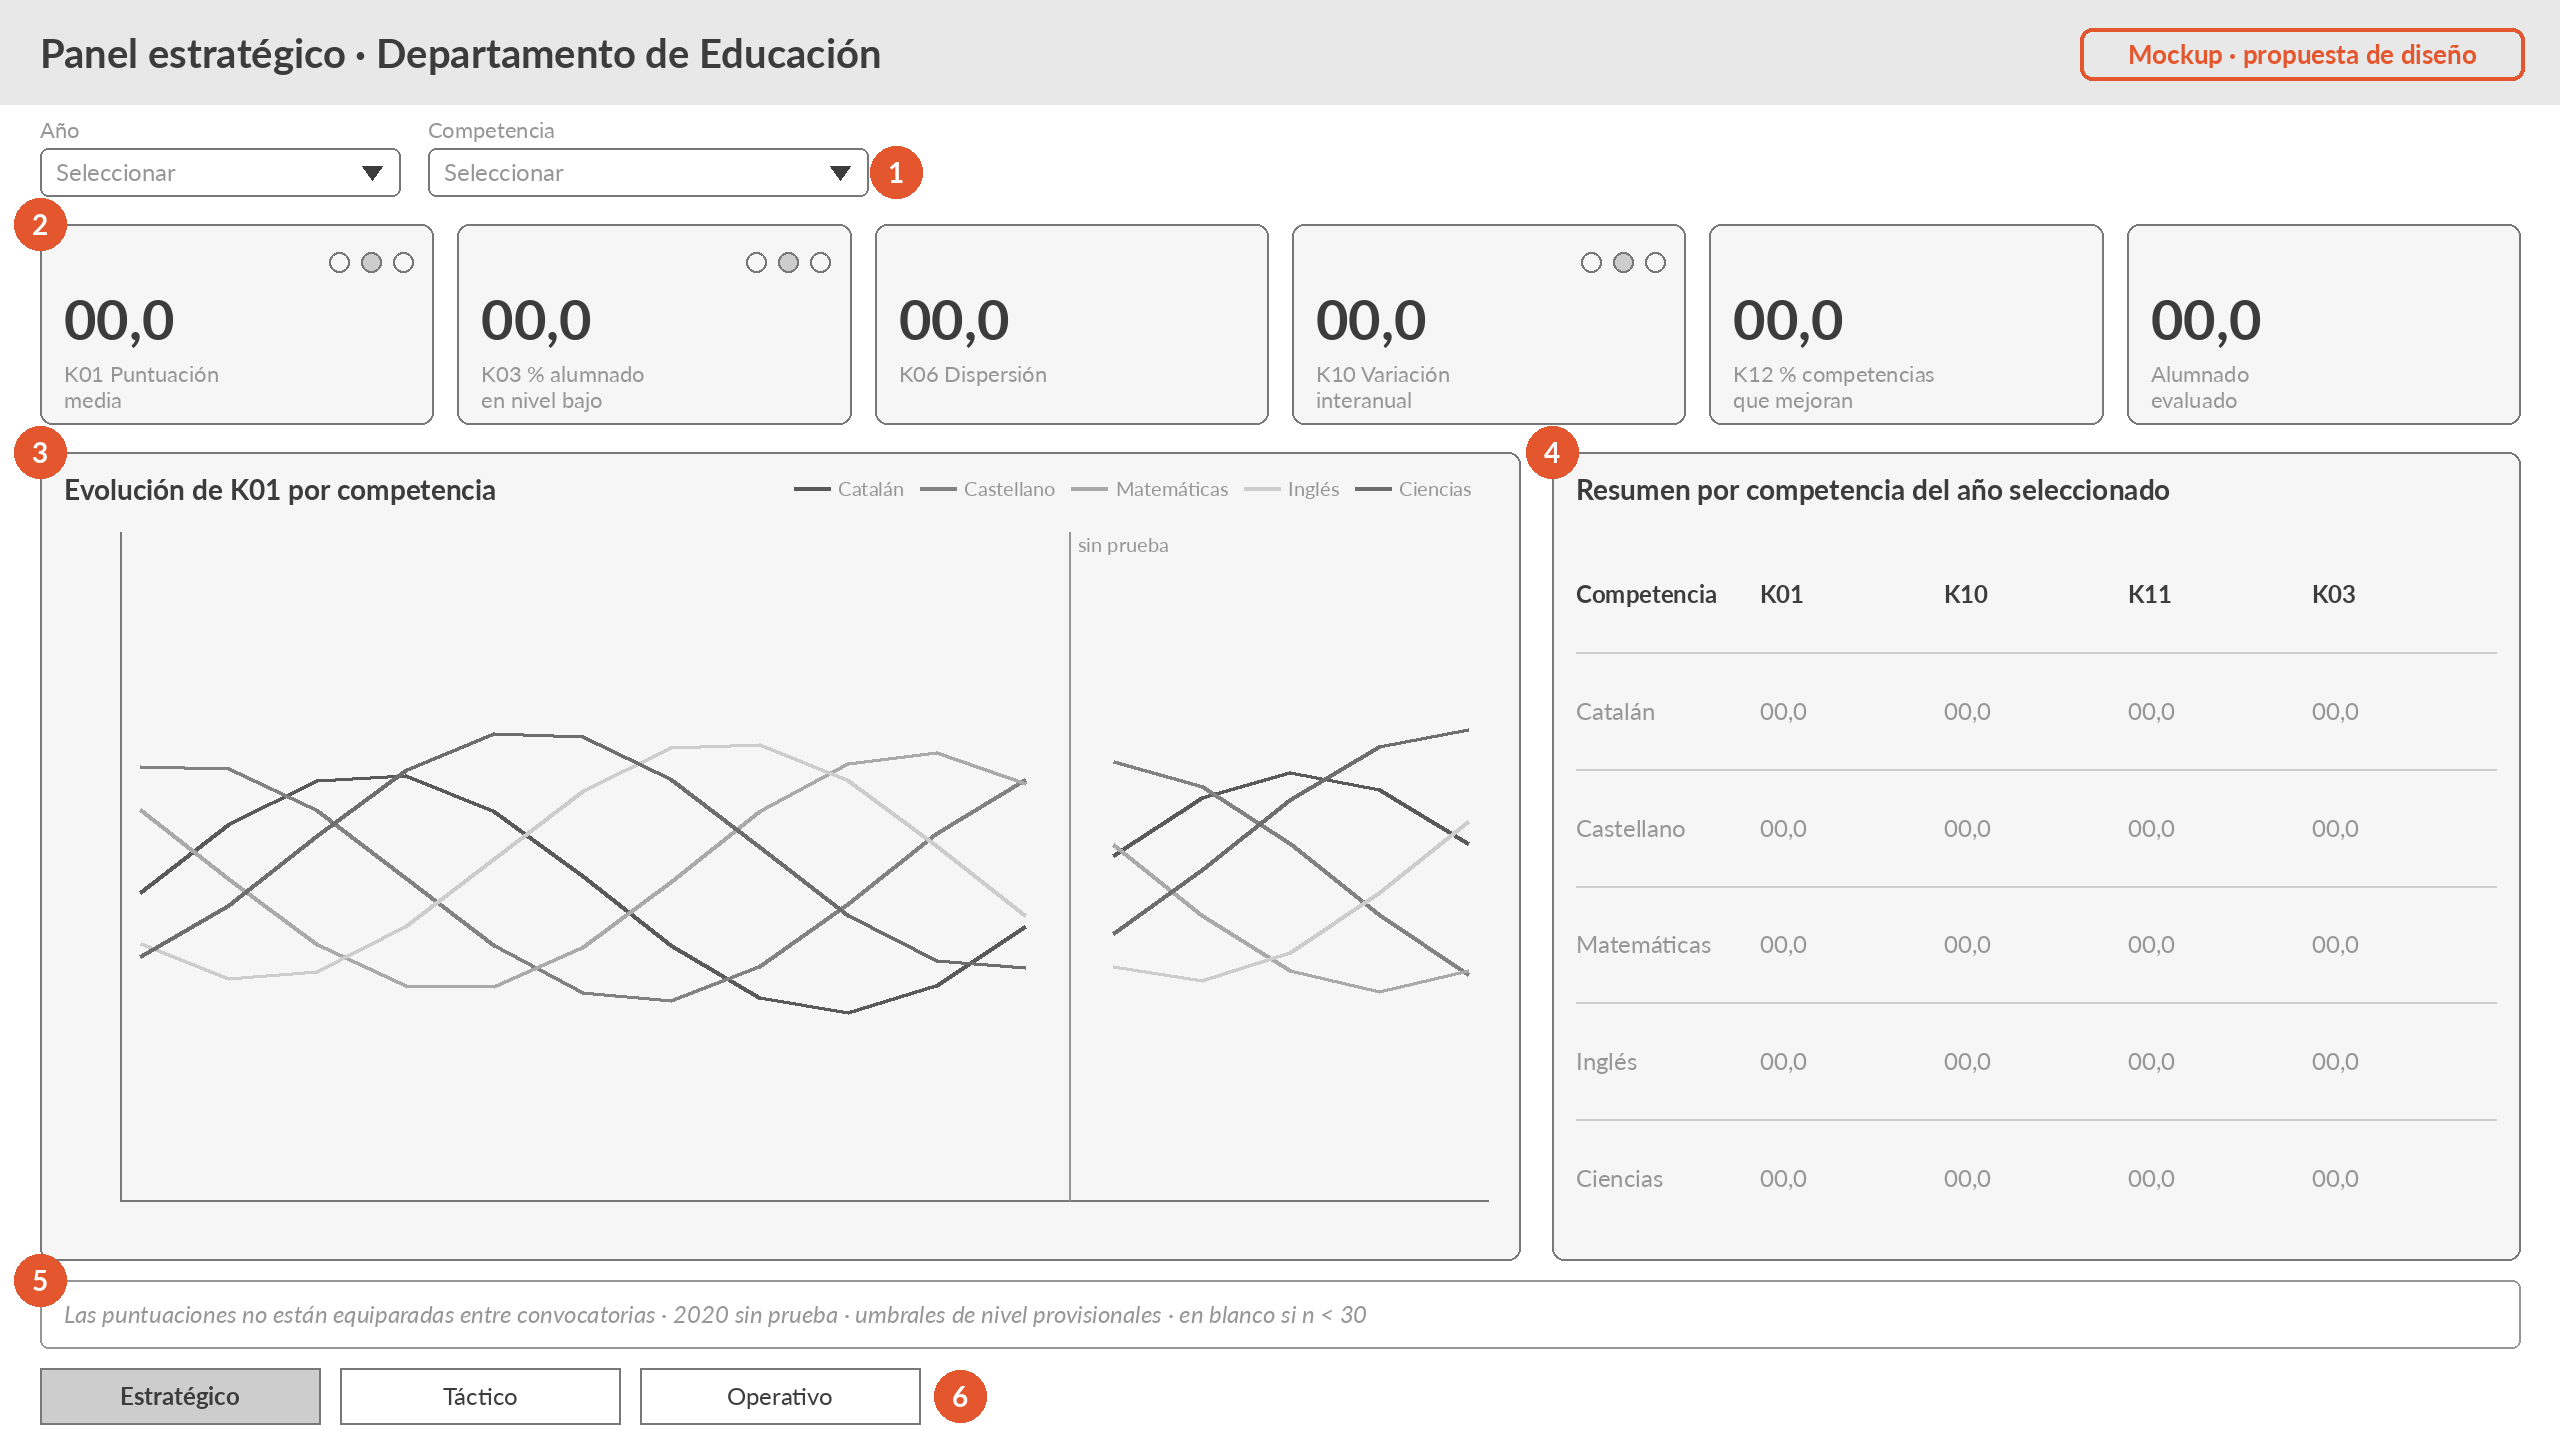
\includegraphics[width=\textwidth]{imagenes/mockups/mockup_estrategico.png}
\caption{Mockup del panel estratégico (Departamento de Educación).}
\label{fig:mockup_estrategico}
\end{figure}

El panel estratégico (Figura~\ref{fig:mockup_estrategico}) dará al Departamento de Educación una visión global de Cataluña (RF16):
\begin{enumerate}
    \item Filtros de año y competencia. El año será de selección única y se abrirá en la última convocatoria.
    \item Tarjetas con la puntuación media (K01), el alumnado en nivel bajo (K03), la dispersión (K06), la variación respecto a la convocatoria anterior (K10), el porcentaje de competencias que mejoran (K12) y el alumnado evaluado. K01, K03 y K10 mostrarán su estado, que indica si el valor es favorable, neutro o desfavorable (RF13).
    \item Evolución de K01 por competencia en todas las convocatorias, sea cual sea el año elegido (RF08). El año 2020, sin prueba, aparecerá como un hueco señalado.
    \item Tabla del año elegido con K01, K10, K11 y K03 de cada competencia, para ver de un vistazo cuáles empeoran.
    \item Aviso fijo sobre las limitaciones de los datos (RF15).
    \item Pestañas de navegación. La selección de año y competencia se mantendrá al cambiar de panel (RF10).
\end{enumerate}

\begin{figure}[H]
\centering
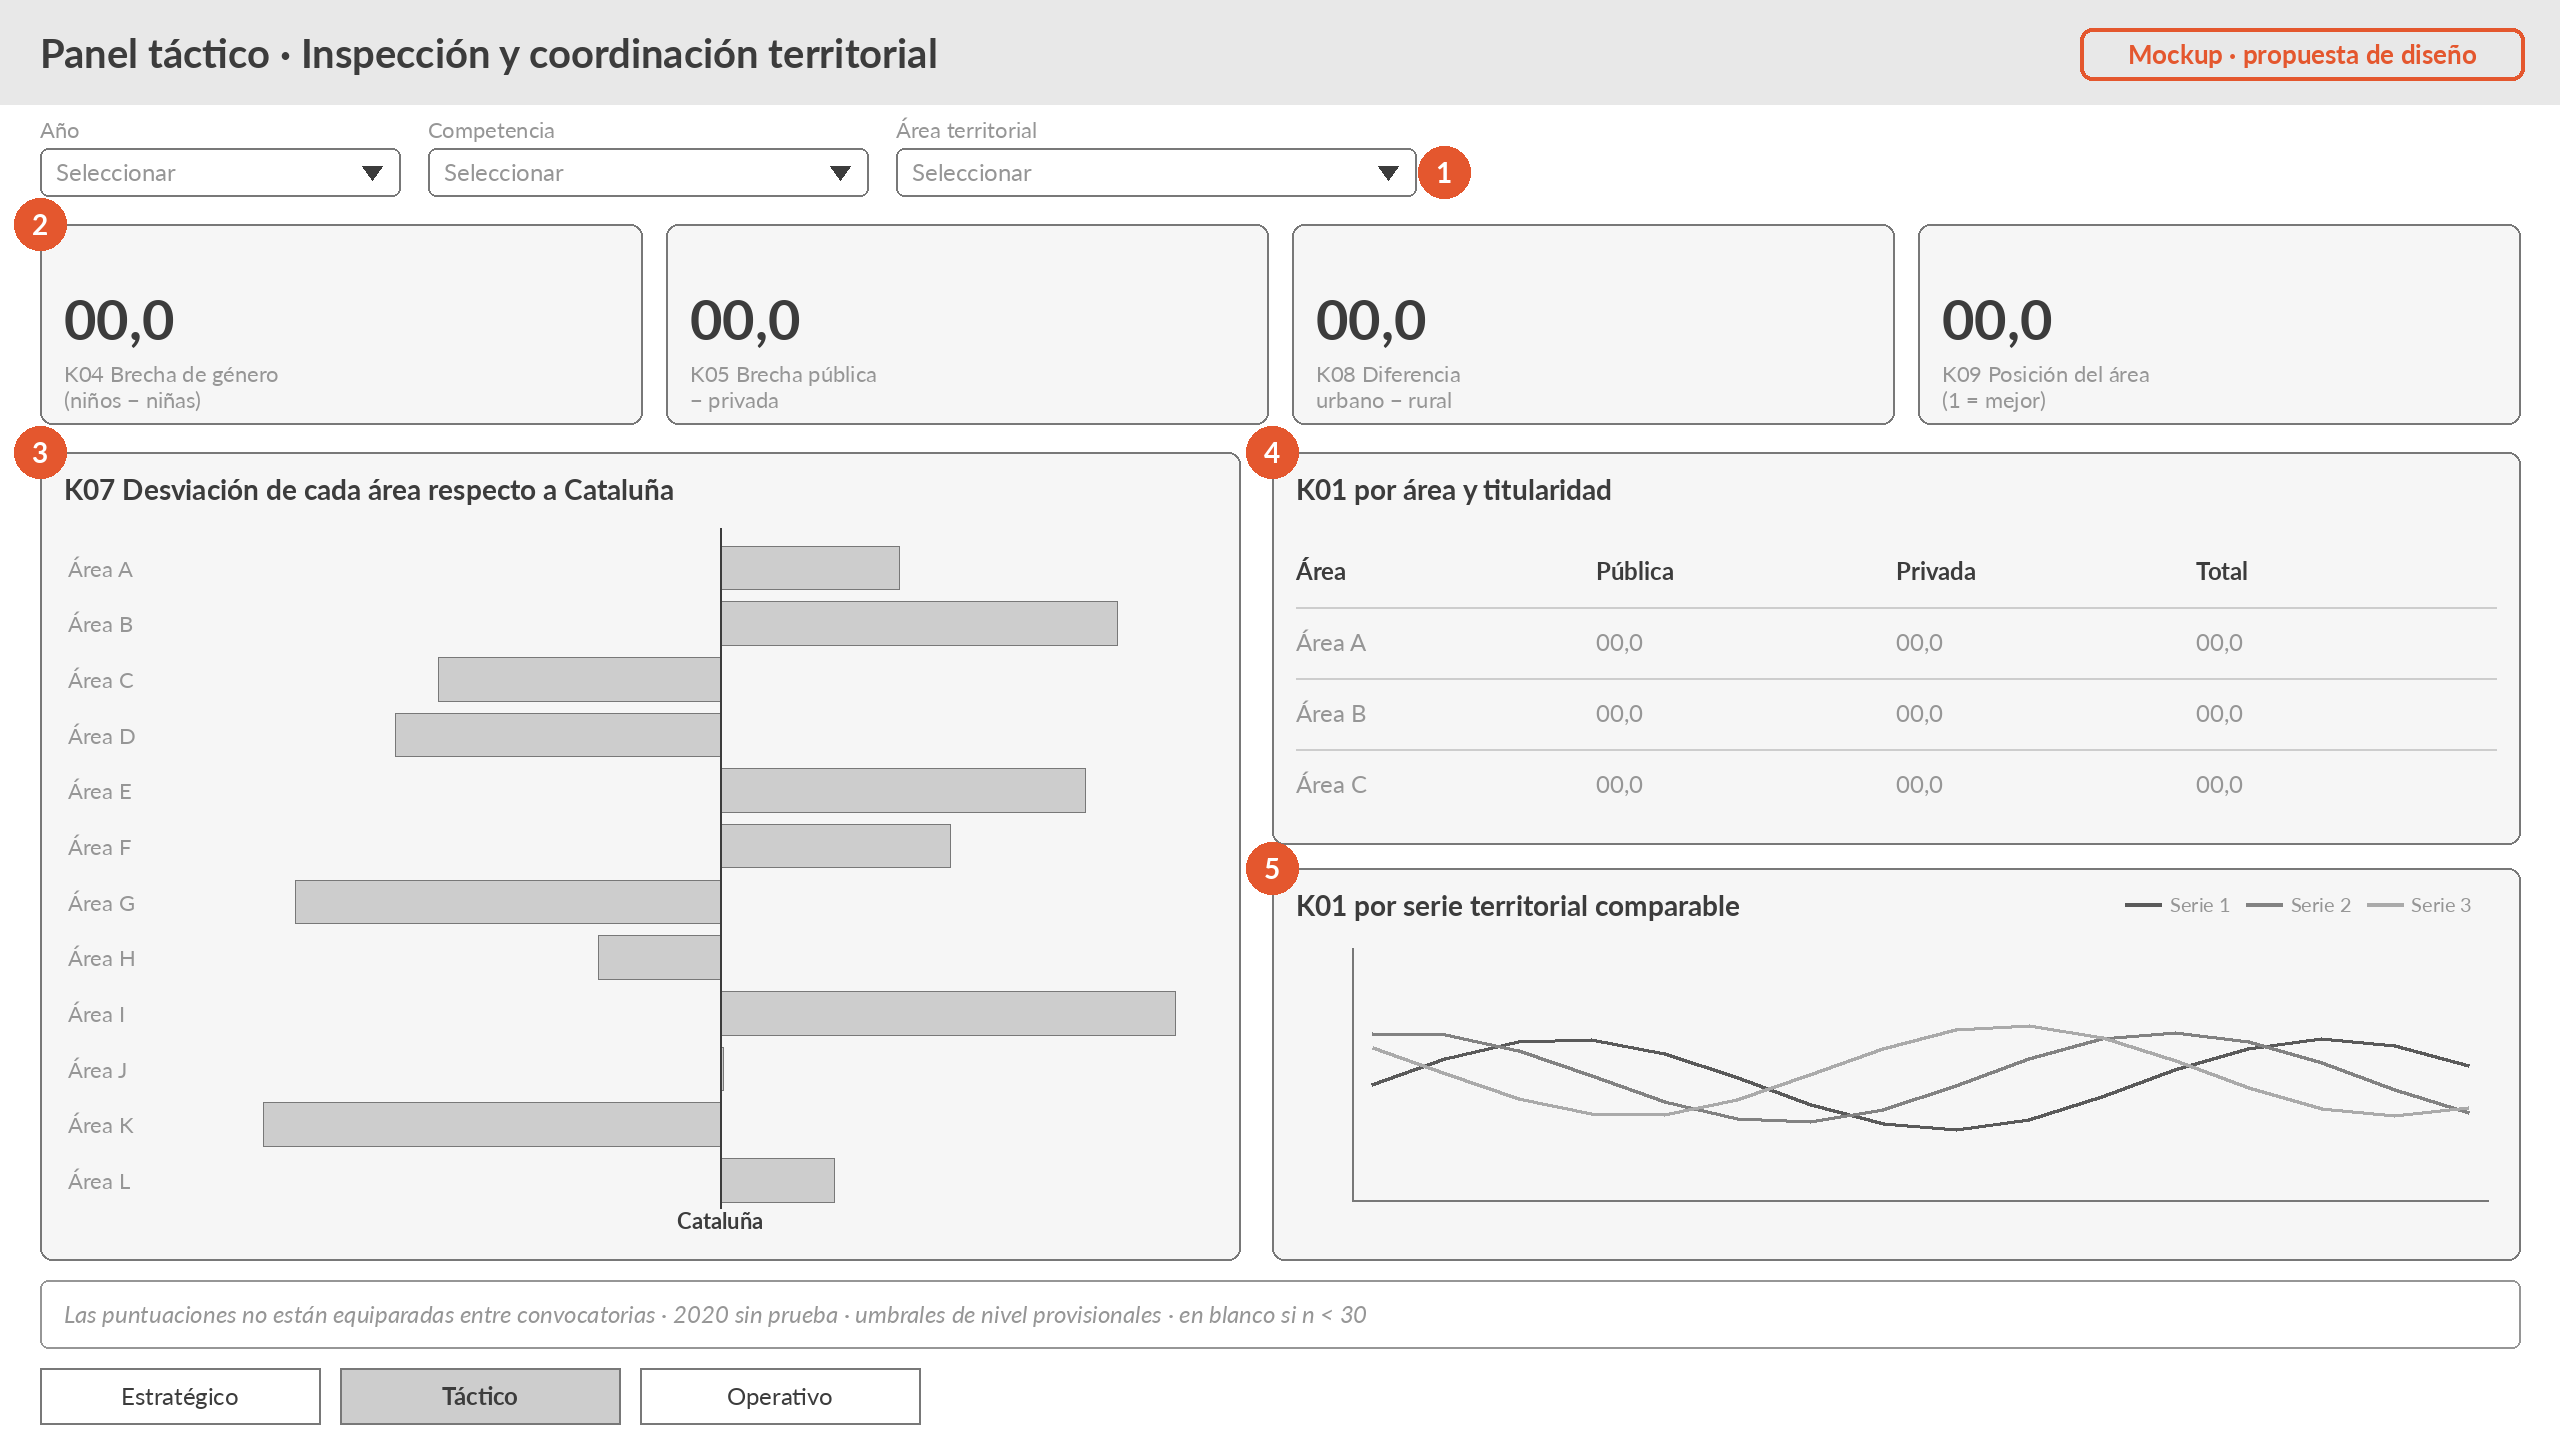
\includegraphics[width=\textwidth]{imagenes/mockups/mockup_tactico.png}
\caption{Mockup del panel táctico (inspección y coordinación territorial).}
\label{fig:mockup_tactico}
\end{figure}

El panel táctico (Figura~\ref{fig:mockup_tactico}) servirá a la inspección para comparar territorios y detectar brechas (RF17):
\begin{enumerate}
    \item Filtros de año, competencia y área territorial.
    \item Tarjetas con la brecha de género (K04), la brecha entre centros públicos y privados (K05), la diferencia entre municipios urbanos y rurales (K08) y la posición del área seleccionada (K09).
    \item Barras con la desviación de cada área respecto a Cataluña (K07). Mostrarán siempre todas las áreas, aunque se filtre una, para no perder la comparación (RF09).
    \item Tabla de K01 por área y titularidad del centro.
    \item Evolución de K01 con las áreas agrupadas en series comparables, ya que la reorganización territorial de 2024 cambió el perímetro de algunas.
\end{enumerate}

\begin{figure}[H]
\centering
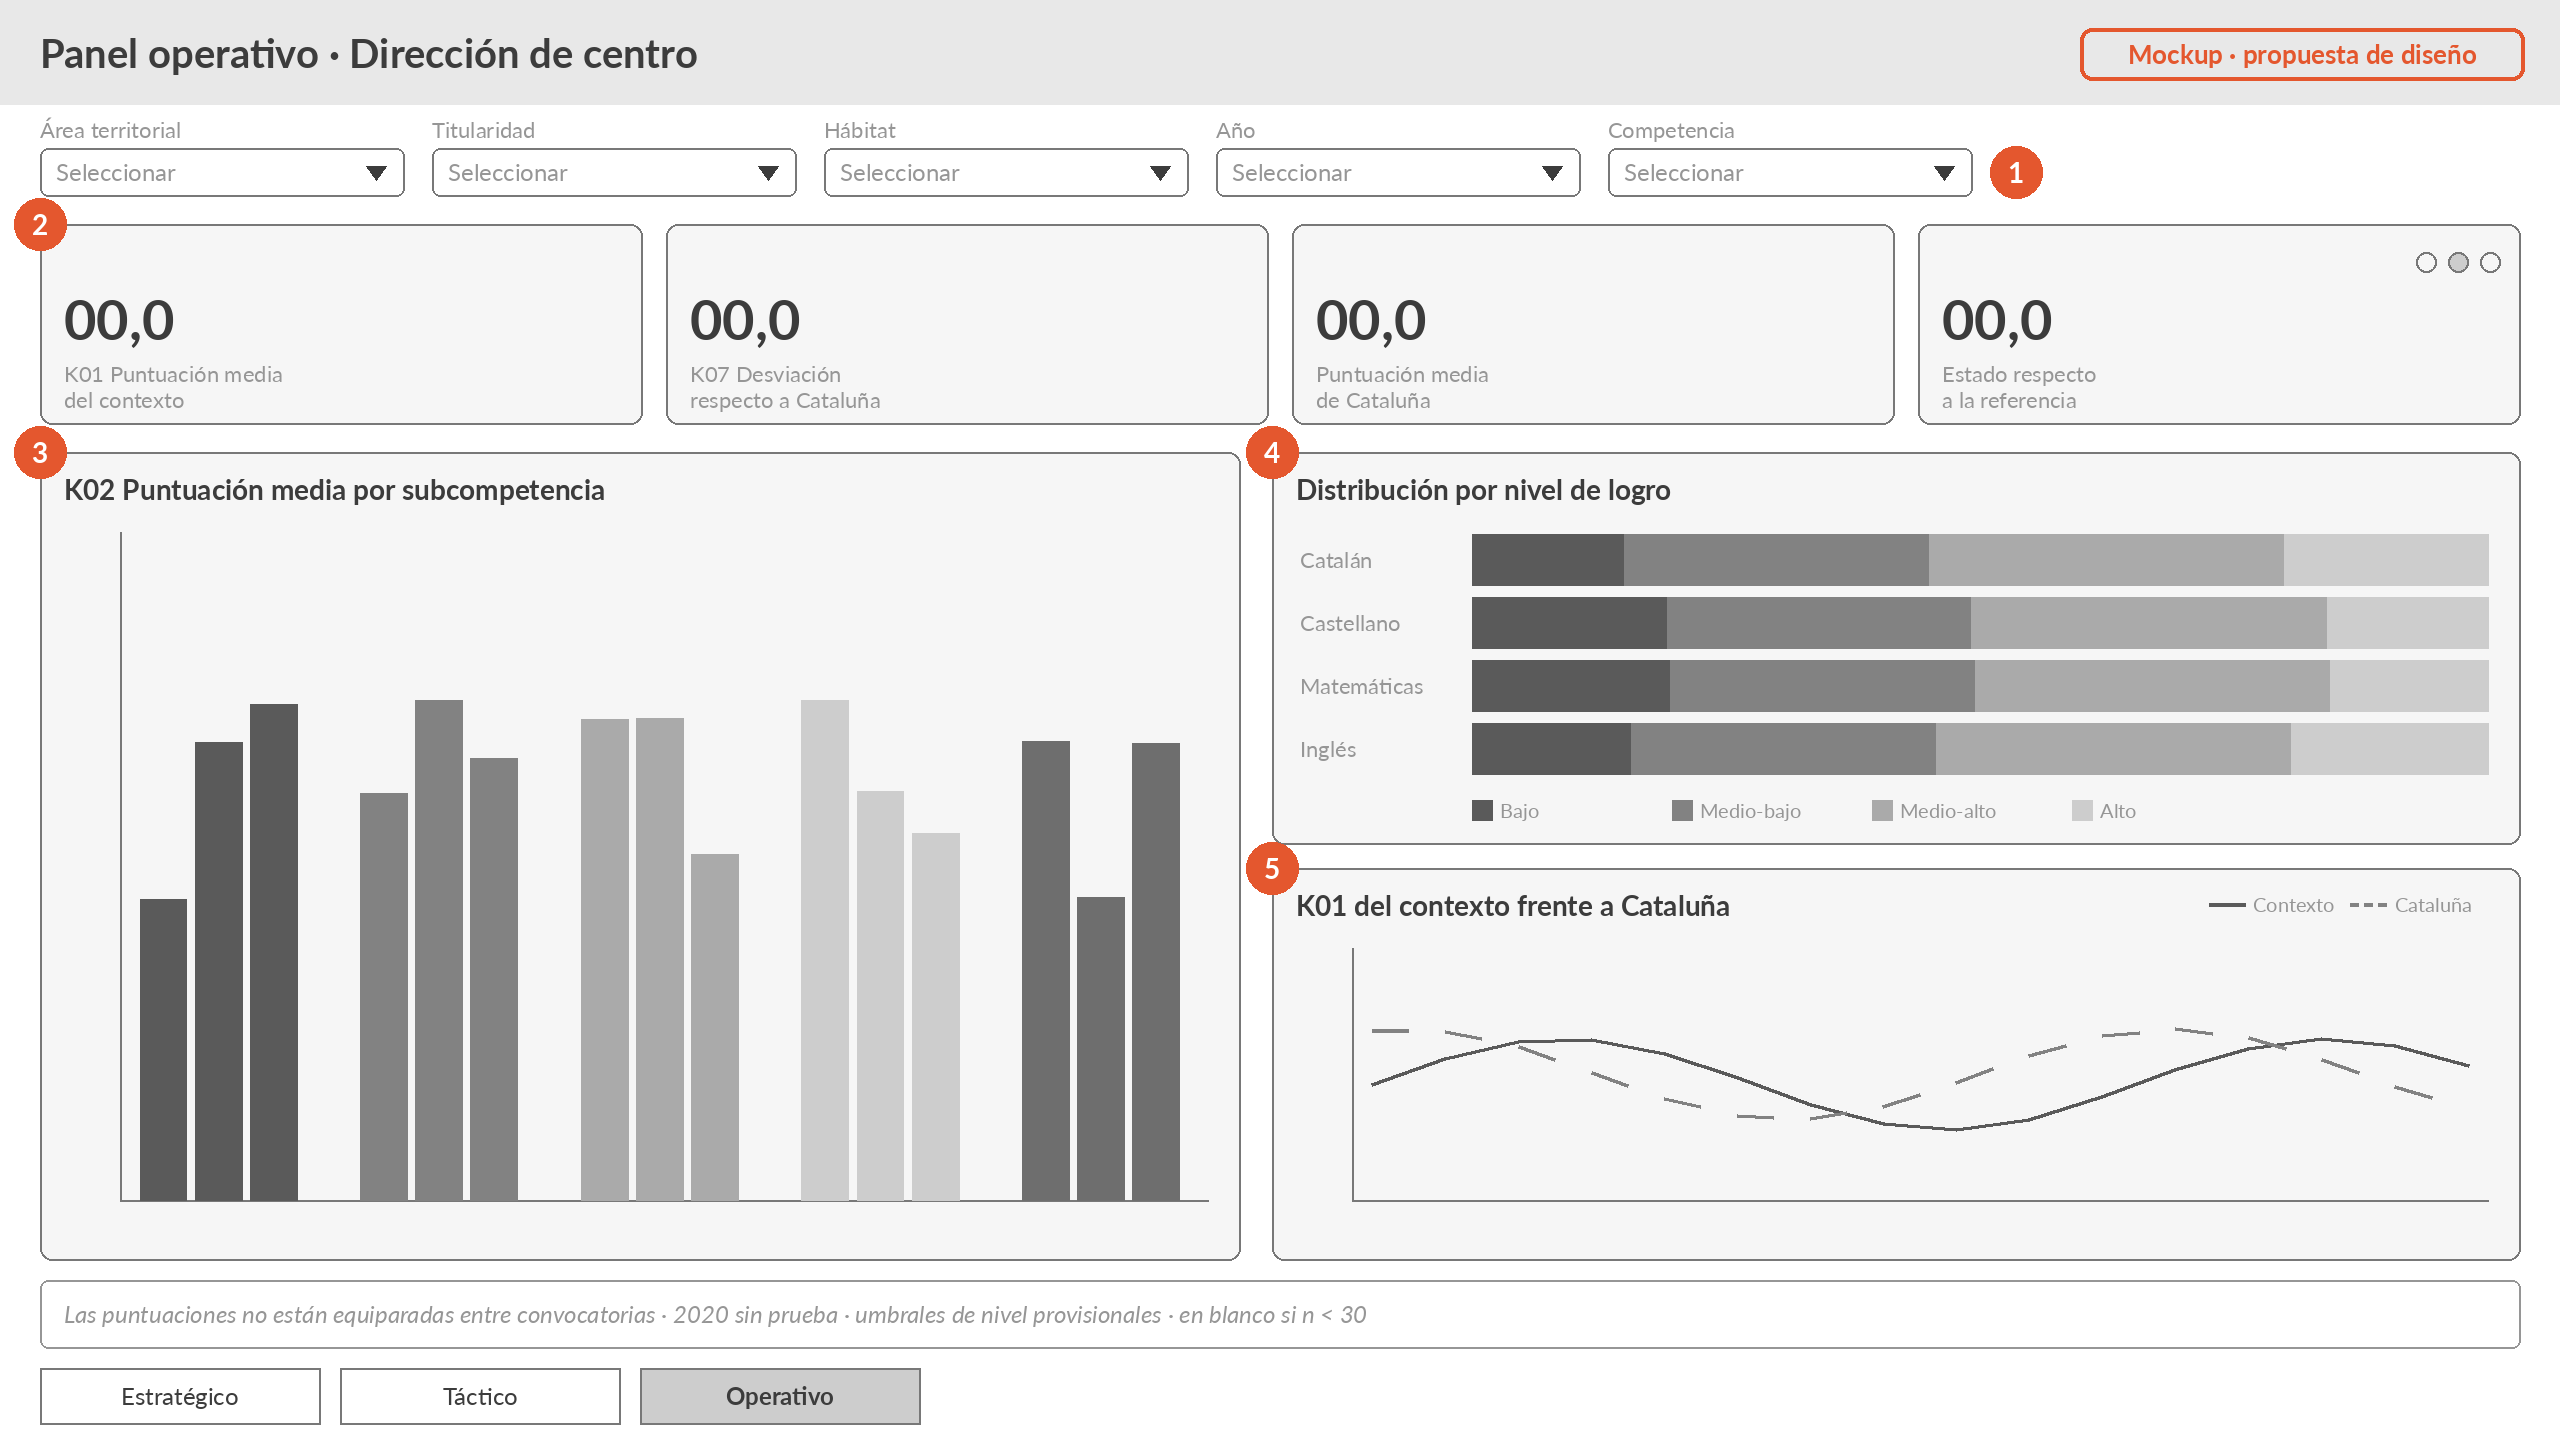
\includegraphics[width=\textwidth]{imagenes/mockups/mockup_operativo.png}
\caption{Mockup del panel operativo (dirección de centro).}
\label{fig:mockup_operativo}
\end{figure}

El panel operativo (Figura~\ref{fig:mockup_operativo}) permitirá a una dirección de centro situar su contexto frente a Cataluña (RF18):
\begin{enumerate}
    \item Filtros de área, titularidad y hábitat para definir el contexto del centro, además del año y la competencia. El panel compara un contexto y no un centro concreto (Sección~\ref{sec:preguntas}).
    \item Tarjetas con K01 del contexto, su desviación respecto a Cataluña (K07), la media de Cataluña como referencia y el estado del KPI.
    \item Puntuación media por subcompetencia (K02), agrupada por competencia (RF07).
    \item Distribución del alumnado por nivel de logro en cada competencia (RF12).
    \item Evolución de K01 del contexto frente a la de Cataluña.
\end{enumerate}

Estos bocetos son el punto de partida del diseño de la interfaz. El diseño final de los paneles y lo que cambia respecto a ellos se recogen en la Sección~\ref{sec:paneles}.

\section{Obstáculos y riesgos}
\label{sec:riesgos}
Una primera exploración del dataset ya ha revelado problemas concretos de calidad: códigos que cambian entre convocatorias (\textit{Públic/Pública}, \textit{H/Home}, \textit{D/Dona}), 13.357 registros de 2024 con valores de hábitat corruptos (\textit{Fins a 10001}, \textit{Fins a 10002}\ldots, típicos de un arrastre en una hoja de cálculo), la ausencia de la convocatoria 2020 y competencias que solo existen en algunos años (inglés desde 2010; ciencias y comprensión oral de catalán y castellano desde 2018). Además, el dataset no incluye un identificador de centro, por lo que el panel operativo ofrecerá una comparación de referencia por contexto y no los resultados de un centro concreto. La Tabla~\ref{tab:riesgos} resume los riesgos identificados; sus planes alternativos se detallan en la Sección~\ref{sec:planesB}.

\begin{table}[H]
\centering
\small
\renewcommand{\arraystretch}{1.1}
\begin{tabularx}{\textwidth}{@{} c X c c @{}}
\toprule
\textbf{Código} & \textbf{Riesgo} & \textbf{Probabilidad} & \textbf{Impacto} \\ \midrule
R1 & Inconsistencias en los datos fuente mayores de lo previsto & Media (30\%) & Alto \\
R2 & Rendimiento insuficiente del modelo (más de 3 s) & Baja (20\%) & Medio \\
R3 & Subestimación del tiempo de redacción de la memoria & Alta (40\%) & Medio \\
R4 & Baja disponibilidad de usuarios reales para la prueba de usabilidad & Alta (40\%) & Medio \\
R5 & Avería o pérdida del equipo de trabajo & Muy baja (5\%) & Alto \\
R6 & Desviación de la planificación por un alcance excesivo & Media (30\%) & Alto \\ \bottomrule
\end{tabularx}
\caption{Riesgos identificados, probabilidad estimada e impacto.}
\label{tab:riesgos}
\end{table}

% ------------------------------------------
% CAPÍTULO 4: METODOLOGÍA Y RIGOR
% ------------------------------------------
\chapter{Metodología y rigor}

\section{Metodología de trabajo}
\label{sec:metodologia}
Se adopta un enfoque híbrido que combina el ciclo de vida de Kimball para proyectos de \textit{Data Warehouse} \cite{kimball2008lifecycle} con prácticas de Scrum \cite{schwaber2020scrum}, estudiados en asignaturas de la especialidad. El ciclo de Kimball aporta la secuencia técnica (requisitos, modelo dimensional, ETL, aplicación BI y despliegue), mientras que Scrum aporta iteraciones cortas y la adaptación continua a lo que se descubra sobre los datos.

La adaptación al proyecto es la siguiente: al haber una sola desarrolladora, se trabaja en \textit{sprints} de dos semanas con un \textit{backlog} priorizado según el alcance mínimo de la Tabla~\ref{tab:alcance}. Cada \textit{sprint} empieza con una planificación y termina con una revisión con las directoras (que actúan como \textit{product owner}) en la que se validan los incrementos: perfilado de datos, modelo, ETL, medidas y paneles.

\section{Herramientas de seguimiento}
\begin{itemize}
    \item \textbf{Git y GitHub:} control de versiones del archivo de Power BI (formato \texttt{.pbip}), de las consultas M y DAX, de los scripts auxiliares y de la memoria.
    \item \textbf{GitHub Projects:} tablero Kanban con el \textit{backlog}, las tareas T1--T23 y el registro de horas reales por tarea, que alimenta el control de costes (Sección~\ref{sec:control}).
    \item \textbf{Overleaf / \LaTeX:} redacción de la memoria y de los entregables de GEP con formato bibliográfico IEEE.
    \item \textbf{Reuniones de seguimiento:} quincenales con las directoras.
\end{itemize}

\section{Métodos de validación}
\label{sec:validacion}
Cada subobjetivo tiene un criterio de aceptación verificable:
\begin{itemize}
    \item \textbf{Exactitud de los datos (SO1, SO4):} conteos de registros por convocatoria antes y después de la ETL, y contraste de las medias calculadas con las publicadas en los informes oficiales \cite{csase_resultats} (tolerancia de $\pm 0{,}5$ puntos).
    \item \textbf{Rendimiento (RNF01):} medición de los tiempos de consulta con DAX Studio \cite{dax_studio} y con el analizador de rendimiento de Power BI.
    \item \textbf{Usabilidad (RNF02):} prueba con al menos 5 usuarios con perfiles representativos, tareas guiadas y el cuestionario SUS \cite{brooke1996sus}, complementada con una evaluación heurística \cite{nielsen1993usability}.
    \item \textbf{Alineación estratégica (SO2):} revisión del catálogo de KPIs con las directoras.
\end{itemize}

% ------------------------------------------
% CAPÍTULO 5: PLANIFICACIÓN TEMPORAL
% ------------------------------------------
\chapter{Planificación temporal}

\section{Datos globales del proyecto}
El TFG tiene una carga de 18 créditos ECTS. La normativa española fija entre 25 y 30 horas de trabajo por crédito \cite{boe_rd1125_2003} y la FIB establece 30 horas por crédito para el TFG \cite{fib_normativa_tfg}, por lo que la dedicación total es de \textbf{18 $\times$ 30 = 540 horas}. El proyecto empezó el 15 de septiembre de 2026 y finaliza con la defensa en el periodo ordinario del primer cuatrimestre (19--25 de enero de 2027): 19 semanas, con una media de 28,4 horas semanales.

La dedicación no es uniforme. Se distinguen tres fases (Tabla~\ref{tab:fases}): una fase inicial más ligera, compatible con los entregables de GEP; una fase de desarrollo técnico; y una fase final más intensa, que coincide con las vacaciones de Navidad, sin docencia.

\begin{table}[H]
\centering
\small
\renewcommand{\arraystretch}{1.1}
\begin{tabularx}{\textwidth}{@{} p{1.6cm} p{4.2cm} c c X @{}}
\toprule
\textbf{Fase} & \textbf{Periodo} & \textbf{Semanas} & \textbf{Horas} & \textbf{Foco principal} \\ \midrule
Fase I & 14 sep -- 11 oct 2026 & 1--4 & 94 h & Gestión del proyecto (GEP) y perfilado de datos. \\
Fase II & 12 oct -- 6 dic 2026 & 5--12 & 220 h & Requisitos, KPIs, modelo, ETL y medidas DAX. \\
Fase III & 7 dic 2026 -- 25 ene 2027 & 13--19 & 226 h & Cuadros de mando, validación, cierre y defensa. \\ \midrule
\textbf{Total} & & \textbf{19} & \textbf{540 h} & \textbf{18 ECTS $\times$ 30 h} \\ \bottomrule
\end{tabularx}
\caption{Distribución de la carga de trabajo por fases.}
\label{tab:fases}
\end{table}

\section{Descripción de las tareas}
El trabajo se descompone en 23 tareas codificadas como T1--T23 y agrupadas en siete paquetes. Ninguna supera las 50 horas. Las horas se han estimado de forma ascendente (\textit{bottom-up}) a partir de los entregables de cada tarea. Las tareas de seguimiento (T5) y de redacción de la memoria (T6) se hacen en paralelo con el resto durante todo el proyecto. Las dependencias de precedencia se expresan como $T_i < T_j$ (T$_j$ no puede empezar hasta que termina T$_i$).

\subsection{Gestión del proyecto (T1--T6)}
\begin{itemize}
    \item \textbf{T1 -- Contextualización y alcance (15 h):} estudio del contexto, estado del arte, objetivos, requisitos y riesgos. Recursos: bibliografía.
    \item \textbf{T2 -- Planificación temporal (12 h):} definición de tareas, estimaciones, dependencias, Gantt y planes alternativos. Dependencia: T1 $<$ T2.
    \item \textbf{T3 -- Gestión económica y sostenibilidad (12 h):} presupuesto por actividad, control de costes e informe de sostenibilidad. Dependencia: T2 $<$ T3.
    \item \textbf{T4 -- Documento final de GEP (11 h):} integración de los entregables anteriores y de las correcciones recibidas. Dependencia: T3 $<$ T4.
    \item \textbf{T5 -- Seguimiento y control (20 h, semanas 1--19):} reuniones quincenales con las directoras (unos 10 encuentros de 1 h con su preparación) y control semanal de horas, riesgos y desviaciones. Sin dependencias.
    \item \textbf{T6 -- Redacción de la memoria del TFG (50 h, semanas 5--19):} empieza al terminar GEP y documenta cada incremento a medida que se completa (unas 3,3 h/semana). Dependencia: T4 $<$ T6.
\end{itemize}

\subsection{Análisis y requisitos (T7--T9)}
\begin{itemize}
    \item \textbf{T7 -- Perfilado y auditoría del dataset (30 h):} análisis exploratorio de las 32 columnas por convocatoria, nulos, dominios de valores y anomalías. Recursos: Python (pandas) y Power Query.
    \item \textbf{T8 -- Análisis de requisitos por perfil (20 h):} definición de los perfiles de usuario, de sus preguntas de negocio y de las historias de usuario. Dependencia: T1 $<$ T8.
    \item \textbf{T9 -- Catálogo de KPIs del CMI (25 h):} ficha formal de los 12 KPIs (fórmula, objetivo, perspectiva y umbrales). Dependencias: T7, T8 $<$ T9.
\end{itemize}

\subsection{Diseño (T10--T11)}
\begin{itemize}
    \item \textbf{T10 -- Diseño del modelo dimensional (25 h):} granularidad, tabla de hechos, dimensiones y diccionario de datos (diagramas con draw.io). Dependencia: T9 $<$ T10.
    \item \textbf{T11 -- Prototipado UX/UI (20 h):} bocetos de los tres paneles según buenas prácticas de diseño de cuadros de mando \cite{few2006information} (Figma). Dependencia: T9 $<$ T11.
\end{itemize}

\subsection{Implementación de la ETL (T12--T13)}
\begin{itemize}
    \item \textbf{T12 -- ETL I: extracción, limpieza y homogeneización (35 h):} carga del CSV, tipado, conversión de la coma decimal, unificación de códigos y corrección de los valores anómalos. Dependencia: T7 $<$ T12.
    \item \textbf{T13 -- ETL II: dimensiones, hechos y carga (30 h):} despivotado de competencias, generación de claves sustitutas, construcción de la estrella y verificación de conteos. Dependencias: T10, T12 $<$ T13.
\end{itemize}

\subsection{Lógica analítica en DAX (T14--T15)}
\begin{itemize}
    \item \textbf{T14 -- Medidas DAX base (40 h):} medias, distribuciones por nivel de logro y brechas de género y titularidad. Dependencia: T13 $<$ T14.
    \item \textbf{T15 -- Inteligencia temporal y comparativas (30 h):} variaciones interanuales, tendencias y desviaciones respecto a Cataluña. Dependencia: T14 $<$ T15.
\end{itemize}

\subsection{Cuadros de mando (T16--T18)}
\begin{itemize}
    \item \textbf{T16 -- Panel estratégico del Departamento (25 h):} visión global del CMI y estado de los KPIs por perspectiva. Dependencias: T11, T14 $<$ T16.
    \item \textbf{T17 -- Panel táctico de Inspección (25 h):} comparativas territoriales, de equidad y \textit{drill-down}. Dependencias: T15, T16 $<$ T17.
    \item \textbf{T18 -- Panel operativo de Dirección de centro (20 h):} comparación con centros de contexto similar. Dependencias: T15, T16 $<$ T18.
\end{itemize}

\subsection{Validación (T19--T21)}
\begin{itemize}
    \item \textbf{T19 -- Optimización del rendimiento (20 h):} medición con DAX Studio, reducción de cardinalidad y refactorización de medidas. Dependencias: T17, T18 $<$ T19.
    \item \textbf{T20 -- Validación analítica de los KPIs (15 h):} contraste con los informes oficiales. Dependencia: T15 $<$ T20.
    \item \textbf{T21 -- Prueba de usabilidad (15 h):} sesiones con usuarios y cuestionario SUS. Dependencias: T17, T18 $<$ T21.
\end{itemize}

\subsection{Cierre (T22--T23)}
\begin{itemize}
    \item \textbf{T22 -- Revisión final de la memoria (20 h):} integración de resultados, conclusiones y correcciones de las directoras. Dependencias: T19, T20 $<$ T22.
    \item \textbf{T23 -- Preparación de la defensa (25 h):} presentación, demostración y ensayos cronometrados. Dependencias: T19, T20 $<$ T23.
\end{itemize}

\section{Recursos}
\textbf{Recursos humanos:} la estudiante desempeña todos los roles del proyecto (jefa de proyecto, analista, ingeniera de datos, desarrolladora BI, especialista en QA y redactora técnica), con la supervisión de las directoras del TFG. La Tabla~\ref{tab:resumen_tareas} asigna un rol a cada tarea, asignación que se usa en el presupuesto.

\textbf{Recursos materiales:} portátil ASUS TUF Gaming F15 con monitor externo; Power BI Desktop, Power Query, DAX Studio, Python (pandas), draw.io, Figma (plan gratuito), Git y GitHub, y Overleaf; conexión a Internet y espacio de trabajo propio.

\section{Resumen de tareas}
La Tabla~\ref{tab:resumen_tareas} resume las tareas con su código, horas, semanas, dependencias y recursos.

\begin{table}[H]
\centering
\footnotesize
\renewcommand{\arraystretch}{1.0}
\setlength{\tabcolsep}{3.5pt}
\begin{tabularx}{\textwidth}{@{} l X c c l l @{}}
\toprule
\textbf{Cód.} & \textbf{Tarea} & \textbf{Horas} & \textbf{Sem.} & \textbf{Dependencias} & \textbf{Rol / recursos} \\ \midrule
T1 & Contextualización y alcance & 15 & 1--2 & -- & PM \\
T2 & Planificación temporal & 12 & 2--3 & T1 & PM \\
T3 & Gestión económica y sostenibilidad & 12 & 3--4 & T2 & PM \\
T4 & Documento final de GEP & 11 & 4 & T3 & PM, \LaTeX \\
T5 & Seguimiento y control & 20 & 1--19 & -- & PM, directoras \\
T6 & Redacción de la memoria & 50 & 5--19 & T4 & RT, Overleaf \\
T7 & Perfilado y auditoría del dataset & 30 & 1--3 & -- & ID, Python \\
T8 & Análisis de requisitos por perfil & 20 & 4--5 & T1 & AN \\
T9 & Catálogo de KPIs del CMI & 25 & 6--7 & T7, T8 & AN, directoras \\
T10 & Diseño del modelo dimensional & 25 & 8 & T9 & ID, draw.io \\
T11 & Prototipado UX/UI & 20 & 9--10 & T9 & BI, Figma \\
T12 & ETL I: limpieza y homogeneización & 35 & 5--7 & T7 & ID, Power Query \\
T13 & ETL II: dimensiones, hechos y carga & 30 & 9--10 & T10, T12 & ID, Power Query \\
T14 & Medidas DAX base & 40 & 11--12 & T13 & BI, Power BI \\
T15 & Inteligencia temporal y comparativas & 30 & 13--14 & T14 & BI, Power BI \\
T16 & Panel estratégico (Departamento) & 25 & 13--14 & T11, T14 & BI, Power BI \\
T17 & Panel táctico (Inspección) & 25 & 15--16 & T15, T16 & BI, Power BI \\
T18 & Panel operativo (Dirección de centro) & 20 & 15--16 & T15, T16 & BI, Power BI \\
T19 & Optimización del rendimiento & 20 & 17 & T17, T18 & BI, DAX Studio \\
T20 & Validación analítica de KPIs & 15 & 15--16 & T15 & QA, informes oficiales \\
T21 & Prueba de usabilidad & 15 & 17--18 & T17, T18 & QA, usuarios \\
T22 & Revisión final de la memoria & 20 & 18--19 & T19, T20 & RT, directoras \\
T23 & Preparación de la defensa & 25 & 18--19 & T19, T20 & PM \\ \midrule
\multicolumn{2}{@{}l}{\textbf{Total}} & \textbf{540} & & & \\ \bottomrule
\end{tabularx}
\caption{Resumen de tareas, horas, semanas, dependencias y recursos. Roles: PM (jefa de proyecto), AN (analista), ID (ingeniera de datos), BI (desarrolladora BI), QA (validación), RT (redactora técnica).}
\label{tab:resumen_tareas}
\end{table}

\section{Diagrama de Gantt}
La Figura~\ref{fig:gantt} muestra el calendario en semanas. La concurrencia es explícita: T5 y T6 se desarrollan en paralelo al resto; T12 (limpieza) se adelanta al diseño del modelo porque solo depende del perfilado; T11 avanza en paralelo con la ETL; y T20 valida los KPIs mientras se construyen los paneles. La carga semanal resultante oscila entre 19 y 34 horas.

\begin{landscape}
\begin{figure}[p]
\centering
\begin{adjustbox}{max width=\linewidth, max totalheight=0.93\textheight}
\begin{ganttchart}[
    vgrid={*1{dotted}},
    hgrid,
    x unit=0.9cm,
    y unit chart=0.42cm,
    title/.style={fill=gray!20, draw=black},
    title label font=\bfseries\footnotesize,
    bar/.style={fill=blue!35, draw=black},
    bar height=0.6,
    bar label font=\footnotesize,
    group/.style={fill=black},
    group height=0.25,
    group label font=\bfseries\footnotesize,
    milestone/.style={fill=red!70, draw=black},
    milestone label font=\itshape\footnotesize
]{1}{19}
\gantttitle{Sep}{3} \gantttitle{Oct}{4} \gantttitle{Nov}{5} \gantttitle{Dic}{4} \gantttitle{Ene}{3} \\
\gantttitlelist{1,...,19}{1} \\
\ganttgroup{Gestión del proyecto}{1}{19} \\
\ganttbar{T1: Contextualización y alcance}{1}{2} \\
\ganttbar{T2: Planificación temporal}{2}{3} \\
\ganttbar{T3: Gestión económica y sostenibilidad}{3}{4} \\
\ganttbar{T4: Documento final GEP}{4}{4} \\
\ganttbar[bar/.append style={fill=gray!45}]{T5: Seguimiento y control}{1}{19} \\
\ganttbar[bar/.append style={fill=gray!45}]{T6: Redacción de la memoria}{5}{19} \\
\ganttgroup{Análisis y requisitos}{1}{7} \\
\ganttbar[bar/.append style={fill=teal!40}]{T7: Perfilado del dataset}{1}{3} \\
\ganttbar[bar/.append style={fill=teal!40}]{T8: Requisitos por perfil}{4}{5} \\
\ganttbar[bar/.append style={fill=teal!40}]{T9: Catálogo de KPIs}{6}{7} \\
\ganttgroup{Diseño}{8}{10} \\
\ganttbar[bar/.append style={fill=orange!45}]{T10: Modelo dimensional}{8}{8} \\
\ganttbar[bar/.append style={fill=orange!45}]{T11: Prototipado UX/UI}{9}{10} \\
\ganttgroup{ETL y DAX}{5}{14} \\
\ganttbar[bar/.append style={fill=green!40}]{T12: ETL I -- limpieza}{5}{7} \\
\ganttbar[bar/.append style={fill=green!40}]{T13: ETL II -- estrella}{9}{10} \\
\ganttbar[bar/.append style={fill=green!40}]{T14: Medidas DAX base}{11}{12} \\
\ganttbar[bar/.append style={fill=green!40}]{T15: Inteligencia temporal DAX}{13}{14} \\
\ganttgroup{Cuadros de mando}{13}{16} \\
\ganttbar[bar/.append style={fill=violet!35}]{T16: Panel estratégico}{13}{14} \\
\ganttbar[bar/.append style={fill=violet!35}]{T17: Panel táctico}{15}{16} \\
\ganttbar[bar/.append style={fill=violet!35}]{T18: Panel operativo}{15}{16} \\
\ganttgroup{Validación}{15}{18} \\
\ganttbar[bar/.append style={fill=yellow!55}]{T19: Optimización rendimiento}{17}{17} \\
\ganttbar[bar/.append style={fill=yellow!55}]{T20: Validación analítica}{15}{16} \\
\ganttbar[bar/.append style={fill=yellow!55}]{T21: Prueba de usabilidad}{17}{18} \\
\ganttgroup{Cierre}{18}{19} \\
\ganttbar[bar/.append style={fill=red!30}]{T22: Revisión final memoria}{18}{19} \\
\ganttbar[bar/.append style={fill=red!30}]{T23: Preparación de la defensa}{18}{19} \\
\ganttmilestone{H1: Fin de GEP}{4} \\
\ganttmilestone{H2: Modelo y ETL completados}{10} \\
\ganttmilestone{H3: KPIs implementados}{14} \\
\ganttmilestone{H4: Cuadros de mando completados}{16} \\
\ganttmilestone{H5: Defensa (19--25 ene)}{19}
\end{ganttchart}
\end{adjustbox}
\caption{Diagrama de Gantt del proyecto (semanas 1--19, del 14 de septiembre de 2026 al 24 de enero de 2027).}
\label{fig:gantt}
\end{figure}
\end{landscape}

\section{Gestión del riesgo: planes alternativos}
\label{sec:planesB}
Las tareas de los planes B no forman parte de la planificación ni aparecen en el Gantt: solo se activan si el riesgo llega a producirse. En cada reunión de seguimiento (T5) se revisa si aparece alguno de los riesgos definidos, o uno nuevo, y se reajusta la planificación. La Tabla~\ref{tab:planesB} detalla las tareas alternativas, su efecto en la duración y los recursos adicionales.

\begin{table}[H]
\centering
\small
\renewcommand{\arraystretch}{1.1}
\setlength{\tabcolsep}{3pt}
\begin{tabularx}{\textwidth}{@{} c X p{3.2cm} p{2.8cm} @{}}
\toprule
\textbf{Riesgo} & \textbf{Plan B (tareas alternativas)} & \textbf{Impacto en la duración} & \textbf{Recursos adicionales} \\ \midrule
R1 & T12b: reglas adicionales de limpieza; si no basta, acotar el histórico a 2018--2025 (esquema estable). & +20 h en las semanas 6--7; sin retraso de hitos (holgura de T11). & 20 h de ingeniera de datos. \\ \addlinespace
R2 & T19b: precalcular agregados en Power Query y simplificar las medidas más costosas. & +20 h en la semana 17; absorbido por la holgura de las semanas 18--19. & 10 h de ingeniera de datos y 10 h de desarrolladora BI. \\ \addlinespace
R3 & T22b: adelantar capítulos con T6 y usar las vacaciones de Navidad. & +15 h; 0 días de retraso en la defensa. & 15 h de redactora técnica. \\ \addlinespace
R4 & T21b: prueba con perfiles simulados (estudiantes y docentes conocidos) más evaluación heurística \cite{nielsen1993usability}. & +8 h en la semana 18. & 8 h de QA. \\ \addlinespace
R5 & Recuperación desde GitHub en un ordenador de los laboratorios de la FIB. & +6 h; retraso menor de 1 semana. & 6 h; equipos de la FIB. \\ \addlinespace
R6 & Renunciar a las extensiones opcionales y priorizar el alcance mínimo (Tabla~\ref{tab:alcance}). & Recupera la planificación sin horas adicionales. & Ninguno. \\ \bottomrule
\end{tabularx}
\caption{Planes alternativos ante los riesgos identificados.}
\label{tab:planesB}
\end{table}

Con estas medidas, ninguno de los riesgos compromete la defensa en el periodo ordinario.

% ------------------------------------------
% CAPÍTULO 6: GESTIÓN ECONÓMICA
% ------------------------------------------
\chapter{Gestión económica}
\begin{revisado}
El presupuesto sigue la estructura propuesta en la asignatura \cite{fib_costos}: costes de personal por actividad (CPA), costes genéricos (CG), contingencia (C) e imprevistos (I). Se valora como si fuera un encargo profesional.

\section{Costes de personal por actividad (CPA)}
El coste por hora de cada rol parte del salario bruto anual (SBA) de mercado en Barcelona \cite{glassdoor_barcelona}, al que se suma un 30\% de cotizaciones a la Seguridad Social a cargo de la empresa, repartido entre 1.760 horas laborables anuales:
\begin{equation}
\text{Coste/hora} = \frac{\text{SBA} \times 1{,}30}{1.760\ \text{h}}
\end{equation}

\begin{table}[H]
\centering
\small
\renewcommand{\arraystretch}{1.05}
\begin{tabularx}{\textwidth}{@{} X r r r r @{}}
\toprule
\textbf{Rol} & \textbf{SBA (\texteuro{})} & \textbf{\texteuro{}/h} & \textbf{Horas} & \textbf{Coste (\texteuro{})} \\ \midrule
Jefa de proyecto (PM) & 45.000 & 33,24 & 95 & 3.157,80 \\
Analista de negocio (AN) & 38.000 & 28,07 & 45 & 1.263,15 \\
Ingeniera de datos (ID) & 39.000 & 28,81 & 120 & 3.457,20 \\
Desarrolladora BI (BI) & 34.000 & 25,11 & 180 & 4.519,80 \\
Especialista en QA (QA) & 30.000 & 22,16 & 30 & 664,80 \\
Redactora técnica (RT) & 26.000 & 19,20 & 70 & 1.344,00 \\ \midrule
\textbf{Total} & & & \textbf{540} & \textbf{14.406,75} \\ \bottomrule
\end{tabularx}
\caption{Tarifas por rol y coste total de personal.}
\label{tab:tarifas}
\end{table}

La Tabla~\ref{tab:cpa} reparte el coste de personal entre las tareas del Gantt.

\begin{table}[H]
\centering
\small
\renewcommand{\arraystretch}{0.95}
\setlength{\tabcolsep}{4pt}
\begin{tabularx}{\textwidth}{@{} l X c r r @{}}
\toprule
\textbf{Tarea} & \textbf{Descripción} & \textbf{Rol} & \textbf{Horas} & \textbf{Coste (\texteuro{})} \\ \midrule
T1 & Contextualización y alcance & PM & 15 & 498,60 \\
T2 & Planificación temporal & PM & 12 & 398,88 \\
T3 & Gestión económica y sostenibilidad & PM & 12 & 398,88 \\
T4 & Documento final de GEP & PM & 11 & 365,64 \\
T5 & Seguimiento y control & PM & 20 & 664,80 \\
T6 & Redacción de la memoria & RT & 50 & 960,00 \\
T7 & Perfilado y auditoría del dataset & ID & 30 & 864,30 \\
T8 & Análisis de requisitos por perfil & AN & 20 & 561,40 \\
T9 & Catálogo de KPIs del CMI & AN & 25 & 701,75 \\
T10 & Diseño del modelo dimensional & ID & 25 & 720,25 \\
T11 & Prototipado UX/UI & BI & 20 & 502,20 \\
T12 & ETL I: limpieza y homogeneización & ID & 35 & 1.008,35 \\
T13 & ETL II: dimensiones, hechos y carga & ID & 30 & 864,30 \\
T14 & Medidas DAX base & BI & 40 & 1.004,40 \\
T15 & Inteligencia temporal y comparativas & BI & 30 & 753,30 \\
T16 & Panel estratégico & BI & 25 & 627,75 \\
T17 & Panel táctico & BI & 25 & 627,75 \\
T18 & Panel operativo & BI & 20 & 502,20 \\
T19 & Optimización del rendimiento & BI & 20 & 502,20 \\
T20 & Validación analítica de KPIs & QA & 15 & 332,40 \\
T21 & Prueba de usabilidad & QA & 15 & 332,40 \\
T22 & Revisión final de la memoria & RT & 20 & 384,00 \\
T23 & Preparación de la defensa & PM & 25 & 831,00 \\ \midrule
\multicolumn{3}{@{}l}{\textbf{Total CPA}} & \textbf{540} & \textbf{14.406,75} \\ \bottomrule
\end{tabularx}
\caption{Costes de personal por actividad (Tarea | Rol | Horas | Coste).}
\label{tab:cpa}
\end{table}

\section{Costes genéricos (CG)}
Siguiendo el método de la asignatura \cite{fib_costos}, cada coste genérico se calcula dividiendo su importe anual entre las horas laborables reales del año (1.760 h) y multiplicando el resultado por las 540 horas del proyecto:
\begin{itemize}
    \item \textbf{Amortización del hardware:} portátil de 800 \texteuro{} amortizado en 4 años (7.040 h): 0,1136 \texteuro{}/h.
    \item \textbf{Software:} todas las herramientas son gratuitas (Power BI Desktop, DAX Studio, Python, Git, draw.io, Figma y Overleaf en sus planes gratuitos): 0 \texteuro{}.
    \item \textbf{Espacio de trabajo:} 8 m$^2$ de vivienda dedicados al proyecto, a un precio de referencia de 23 \texteuro{}/m$^2$ al mes en Barcelona \cite{idealista_barcelona}: 2.208 \texteuro{}/año.
    \item \textbf{Internet:} conexión de fibra a 40 \texteuro{}/mes: 480 \texteuro{}/año.
    \item \textbf{Electricidad:} consumo medido de 85 W (portátil y monitor) a 0,20 \texteuro{}/kWh: 0,017 \texteuro{}/h.
\end{itemize}

\begin{table}[H]
\centering
\small
\renewcommand{\arraystretch}{1.05}
\begin{tabularx}{\textwidth}{@{} X r r @{}}
\toprule
\textbf{Concepto} & \textbf{\texteuro{}/h} & \textbf{Coste imputado (540 h)} \\ \midrule
Amortización del hardware (800 \texteuro{} / 7.040 h) & 0,1136 & 61,36 \texteuro{} \\
Software & 0,0000 & 0,00 \texteuro{} \\
Espacio de trabajo (2.208 \texteuro{} / 1.760 h) & 1,2545 & 677,45 \texteuro{} \\
Internet (480 \texteuro{} / 1.760 h) & 0,2727 & 147,27 \texteuro{} \\
Electricidad (0,085 kWh $\times$ 0,20 \texteuro{}) & 0,0170 & 9,18 \texteuro{} \\ \midrule
\textbf{Total CG} & \textbf{1,6578} & \textbf{895,26 \texteuro{}} \\ \bottomrule
\end{tabularx}
\caption{Costes genéricos imputados al proyecto.}
\label{tab:cg}
\end{table}

\section{Contingencia (C)}
La contingencia cubre errores de estimación no anticipados y se calcula como un porcentaje del coste del proyecto. Según la asignatura, ese porcentaje depende del sector y del nivel de detalle del presupuesto: cuanto más detallado, menor \cite{fib_costos}. Se fija en un \textbf{10\%} por las siguientes razones:
\begin{itemize}
    \item \textbf{No un 5\%:} es el primer proyecto BI de la desarrolladora, el volumen de datos es elevado y la calidad de los datos ya ha mostrado anomalías (Sección~\ref{sec:riesgos}); un 5\% sería insuficiente.
    \item \textbf{No un 15--20\%:} el presupuesto está detallado tarea a tarea, la fuente de datos es fija y pública (sin dependencias de terceros) y los riesgos identificados ya tienen su propia partida de imprevistos.
\end{itemize}
\begin{equation}
C = 0{,}10 \times (\text{CPA} + \text{CG}) = 0{,}10 \times 15.302{,}01 = 1.530{,}20\ \text{euros}
\end{equation}

\section{Imprevistos (I)}
Cada imprevisto se valora con el coste de su plan B (horas adicionales $\times$ tarifa del rol de la Tabla~\ref{tab:planesB}) ponderado por su probabilidad: $I = \sum P(R_i) \times \text{Coste}_{\text{Plan B},i}$. La probabilidad de R1 se eleva al 30\% tras las anomalías ya detectadas en el dataset.

\begin{table}[H]
\centering
\small
\renewcommand{\arraystretch}{1.05}
\setlength{\tabcolsep}{4pt}
\begin{tabularx}{\textwidth}{@{} c X r c r @{}}
\toprule
\textbf{Riesgo} & \textbf{Cálculo del plan B} & \textbf{Coste (\texteuro{})} & \textbf{$P$} & \textbf{Imputado (\texteuro{})} \\ \midrule
R1 & 20 h ID $\times$ 28,81 & 576,20 & 30\% & 172,86 \\
R2 & 10 h ID $\times$ 28,81 + 10 h BI $\times$ 25,11 & 539,20 & 20\% & 107,84 \\
R3 & 15 h RT $\times$ 19,20 & 288,00 & 40\% & 115,20 \\
R4 & 8 h QA $\times$ 22,16 & 177,28 & 40\% & 70,91 \\
R5 & 6 h BI $\times$ 25,11 & 150,66 & 5\% & 7,53 \\
R6 & Reducción de alcance (sin coste) & 0,00 & 30\% & 0,00 \\ \midrule
\multicolumn{4}{@{}l}{\textbf{Total imprevistos}} & \textbf{474,34} \\ \bottomrule
\end{tabularx}
\caption{Cálculo de la partida de imprevistos.}
\label{tab:imprevistos}
\end{table}

\section{Presupuesto total}
\begin{table}[H]
\centering
\small
\renewcommand{\arraystretch}{1.05}
\begin{tabularx}{0.8\textwidth}{@{} X r @{}}
\toprule
\textbf{Partida} & \textbf{Importe (\texteuro{})} \\ \midrule
Costes de personal por actividad (CPA) & 14.406,75 \\
Costes genéricos (CG) & 895,26 \\ \midrule
\textbf{Subtotal (CPA + CG)} & \textbf{15.302,01} \\
Contingencia (10\%) & 1.530,20 \\
Imprevistos & 474,34 \\ \midrule
\textbf{Total sin IVA} & \textbf{17.306,55} \\
IVA (21\%) & 3.634,38 \\ \midrule
\textbf{Total con IVA} & \textbf{20.940,93} \\ \bottomrule
\end{tabularx}
\caption{Presupuesto total del proyecto.}
\label{tab:presupuesto}
\end{table}

\section{Control de gestión}
\label{sec:control}
Las horas reales dedicadas a cada tarea se registran a diario en GitHub Projects. Al cerrar cada tarea, y de forma agregada al final de cada \textit{sprint} (cada dos semanas) y en cada hito del Gantt, se calculan los indicadores siguientes \cite{fib_costos, pmi2021pmbok}, donde $t_e$ y $t_r$ son las tarifas estimada y real, $h_e$ y $h_r$ las horas estimadas y reales, y $C_e$ y $C_r$ los costes estimado y real de una tarea:
\begin{itemize}
    \item \textbf{Desviación en tarifa:} $D_t = (t_e - t_r) \times h_r$.
    \item \textbf{Desviación en eficiencia (consumo):} $D_h = (h_e - h_r) \times t_e$.
    \item \textbf{Desviación total por tarea:} $D = C_e - C_r$, y en porcentaje $D/C_e \times 100$.
    \item \textbf{Índices de valor ganado:} $\text{CPI} = \text{EV}/\text{AC}$ (eficiencia en coste) y $\text{SPI} = \text{EV}/\text{PV}$ (eficiencia en plazo), donde un valor inferior a 1 indica desviación desfavorable.
    \item \textbf{Consumo de reservas:} porcentaje gastado de las partidas de contingencia e imprevistos.
\end{itemize}

Las desviaciones negativas se cubren primero con la partida de imprevistos, si las causa un riesgo identificado, y después con la de contingencia. Como los imprevistos funcionan como un sistema de compensación, lo reservado para los riesgos que no se materialicen puede cubrir a los que sí lo hagan. Si la desviación acumulada supera el 10\% del coste previsto o el CPI o el SPI bajan de 0,9 durante dos \textit{sprints} consecutivos, se revisa el proyecto con las directoras: según la naturaleza del problema, se ajusta el alcance (renunciando primero a las extensiones opcionales) y se replanifica.

\end{revisado}

% ------------------------------------------
% CAPÍTULO 7: ESPECIFICACIÓN
% ------------------------------------------
\chapter{Especificación}
\label{cap:especificacion}
La especificación describe qué hará el sistema desde el punto de vista de quien lo usa, sin entrar todavía en cómo se construye. Parte de los requisitos de la Sección~\ref{sec:requisitos} y los describe desde tres puntos de vista: qué hace cada usuario con el sistema (casos de uso), qué información maneja (modelo conceptual) y cómo se reparten las funciones entre sus partes (arquitectura general). Después detalla los requisitos no funcionales con una ficha para cada uno y termina con las historias de usuario, que traducen todo lo anterior al \textit{backlog} del desarrollo.

\section{Modelo de casos de uso}
\label{sec:casos_uso}
El modelo tiene seis actores (Figura~\ref{fig:casos_uso}). Los actores principales son los tres perfiles de decisión (E, T y O), que se representan como especializaciones de un actor genérico, el usuario del CMI. Este actor reúne lo que puede hacer cualquier perfil: filtrar los resultados, consultar su evolución y cambiar de panel. Cada perfil añade la consulta de su propio panel. La desarrolladora es la única que carga y actualiza los datos, y el Portal de Datos Abiertos interviene como sistema externo porque de él sale el fichero de origen \cite{transparencia_catalunya_2024}. Las directoras del TFG y los beneficiarios indirectos de la Tabla~\ref{tab:stakeholders} no interactúan con el sistema, así que no aparecen en el modelo.

\begin{figure}[H]
\centering
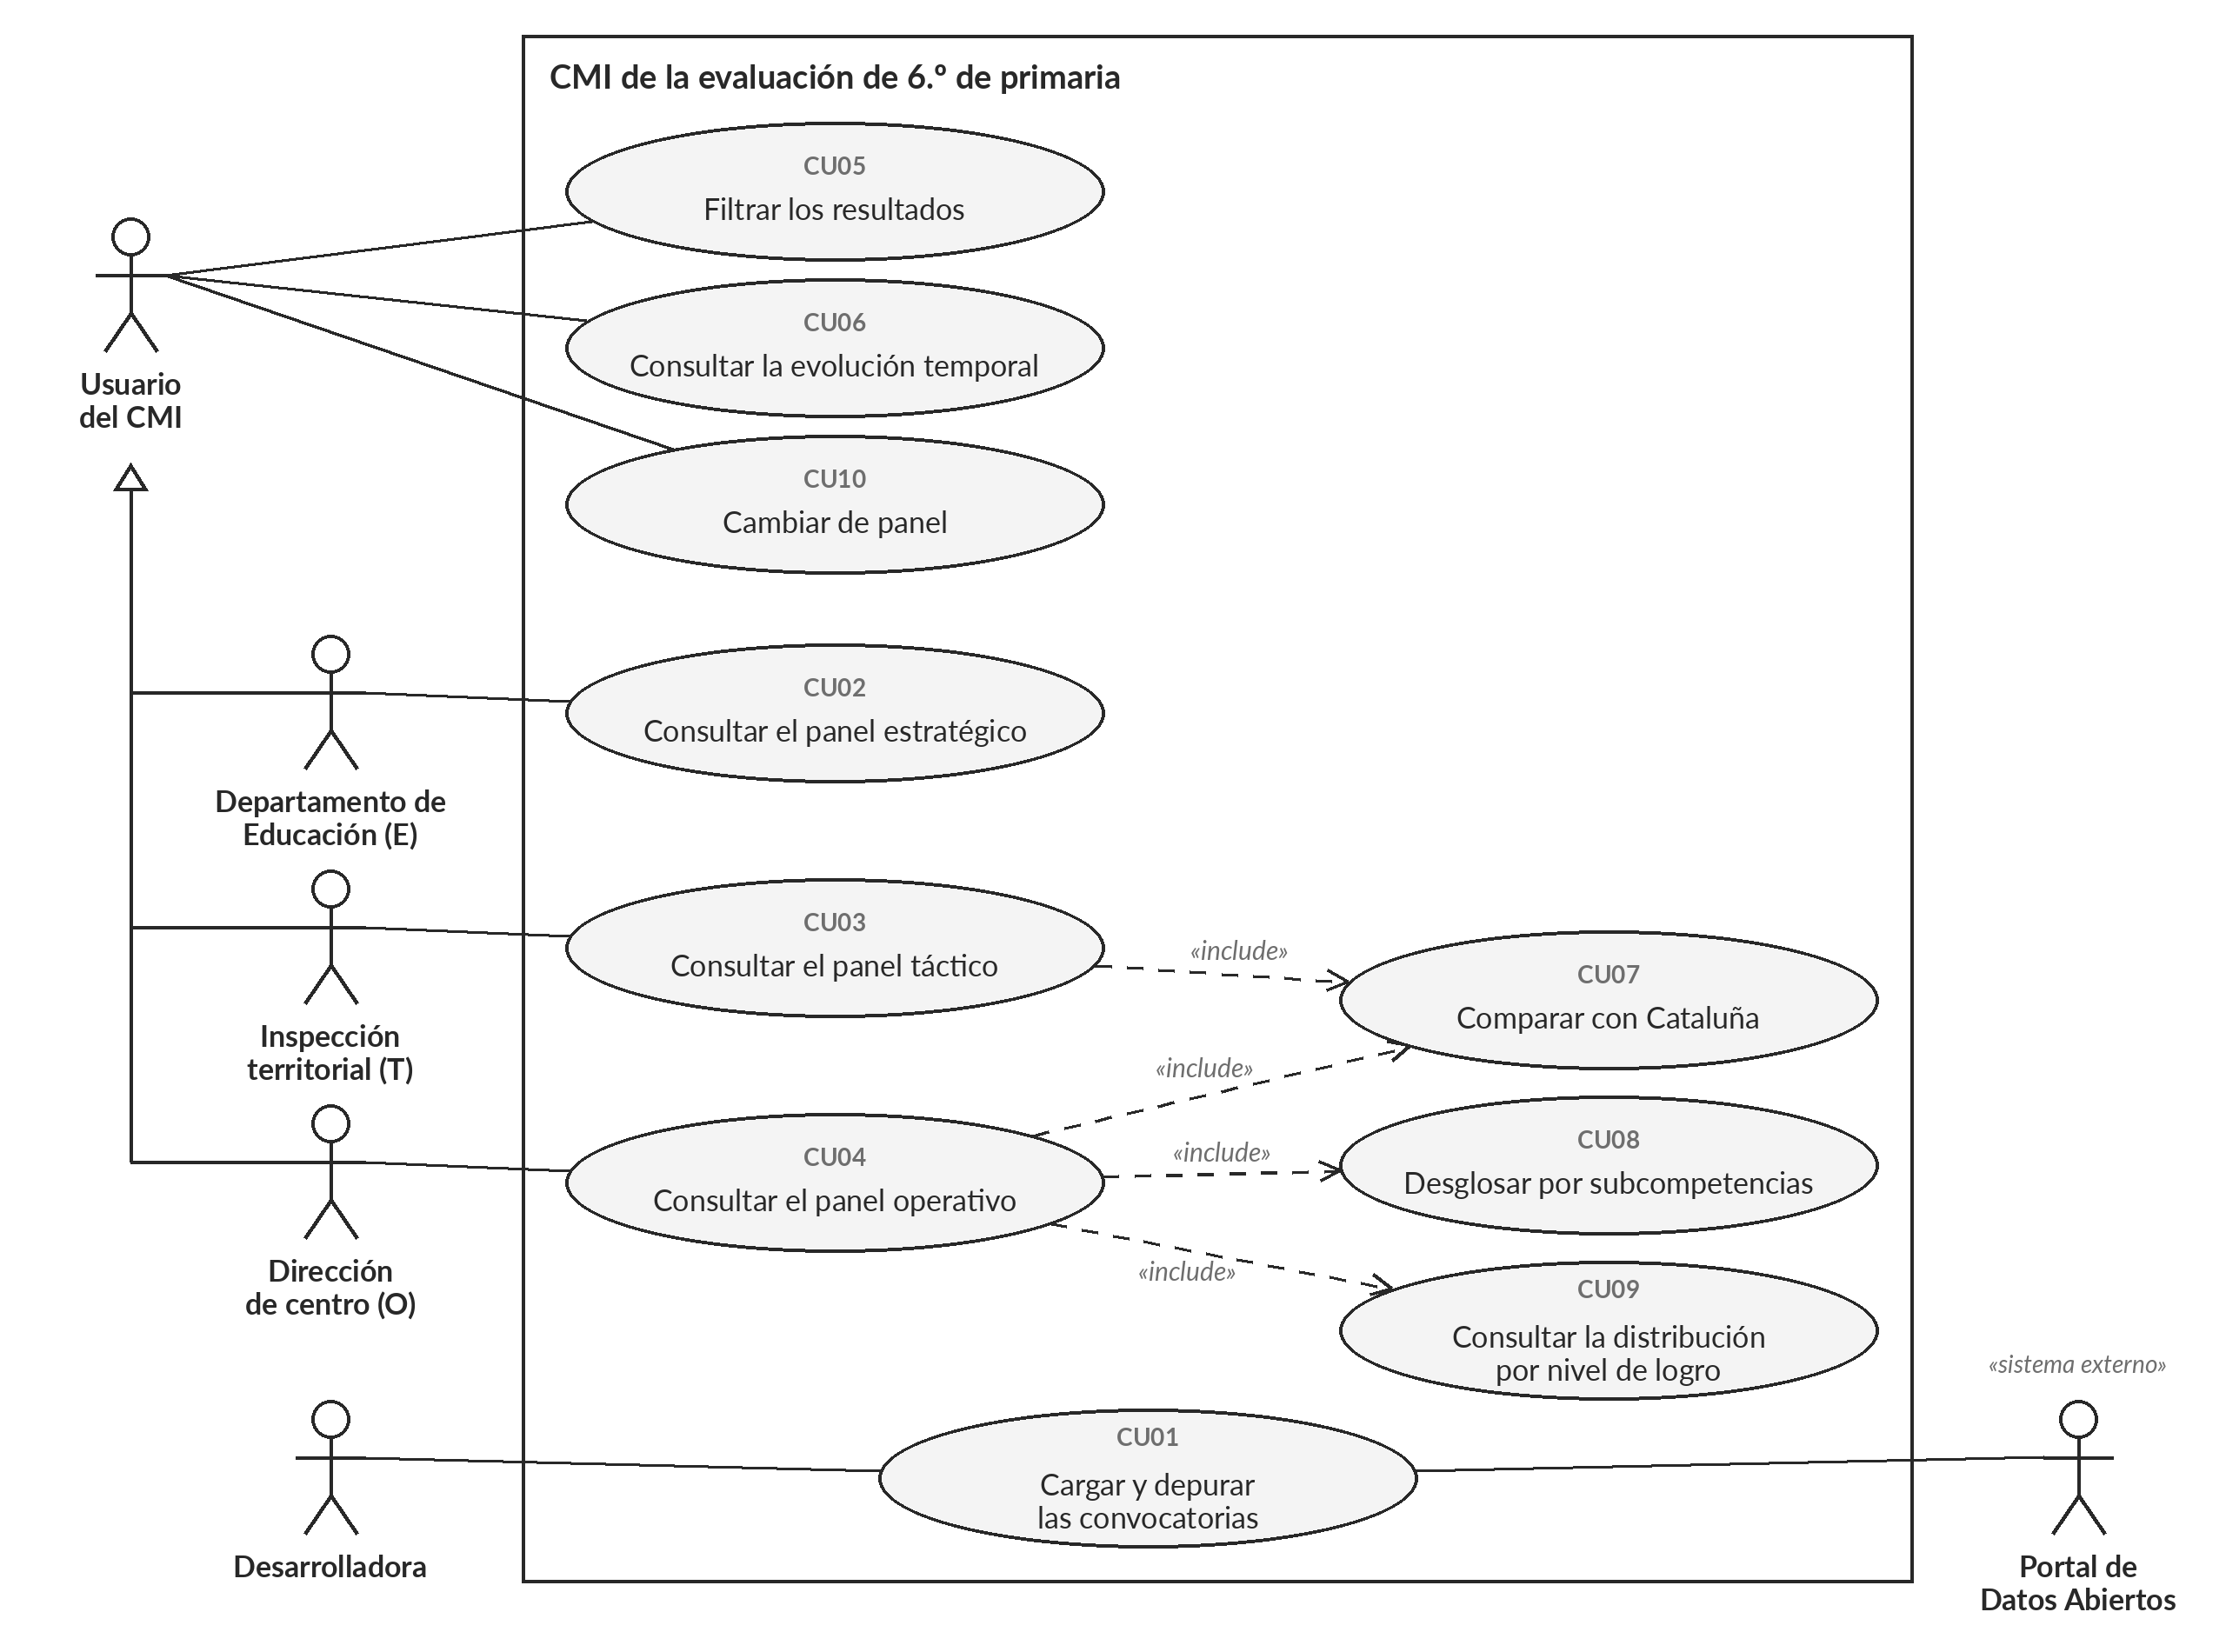
\includegraphics[width=\textwidth]{imagenes/especificacion/casos_uso.png}
\caption{Diagrama de casos de uso.}
\label{fig:casos_uso}
\end{figure}

Los paneles táctico y operativo incluyen la comparación con Cataluña (CU07), porque los dos sitúan un territorio o un contexto frente al total. El panel operativo incluye además el desglose por subcompetencias (CU08) y la distribución del alumnado por nivel de logro (CU09), que muestran en qué falla un contexto concreto. El cálculo de los indicadores, su estado y la regla de las 30 puntuaciones no forman casos de uso propios, porque el usuario no los pide: el sistema los aplica en cada consulta y se describen dentro de los casos que los usan.

La Tabla~\ref{tab:casos_uso} relaciona cada caso de uso con su actor y con los requisitos funcionales que cubre. Cada requisito, de RF01 a RF18, queda cubierto por al menos un caso de uso.

\begin{table}[H]
\centering
\small
\renewcommand{\arraystretch}{1.1}
\begin{tabularx}{\textwidth}{@{} p{1.1cm} X >{\raggedright\arraybackslash}p{3.7cm} >{\raggedright\arraybackslash}p{2.9cm} @{}}
\toprule
\textbf{ID} & \textbf{Caso de uso} & \textbf{Actor} & \textbf{Requisitos} \\ \midrule
CU01 & Cargar y depurar las convocatorias & Desarrolladora y Portal de Datos Abiertos & RF01--RF05 \\ \addlinespace
CU02 & Consultar el panel estratégico & E & RF08, RF11, RF13, RF16 \\ \addlinespace
CU03 & Consultar el panel táctico & T & RF09, RF11, RF13, RF17 \\ \addlinespace
CU04 & Consultar el panel operativo & O & RF07, RF09, RF11--RF14, RF18 \\ \addlinespace
CU05 & Filtrar los resultados & Usuario del CMI & RF06, RF10, RF11, RF14 \\ \addlinespace
CU06 & Consultar la evolución temporal & Usuario del CMI & RF08, RF14, RF15 \\ \addlinespace
CU07 & Comparar con Cataluña & Incluido en CU03 y CU04 & RF09, RF13, RF14 \\ \addlinespace
CU08 & Desglosar por subcompetencias & Incluido en CU04 & RF07, RF14 \\ \addlinespace
CU09 & Consultar la distribución por nivel de logro & Incluido en CU04 & RF04, RF12, RF14 \\ \addlinespace
CU10 & Cambiar de panel & Usuario del CMI & RF10 \\ \bottomrule
\end{tabularx}
\caption{Casos de uso, actores y requisitos funcionales que cubren.}
\label{tab:casos_uso}
\end{table}

\subsection{Descripción de los casos de uso}
Cada caso de uso se describe con una ficha (Tablas~\ref{tab:cu01} a \ref{tab:cu10}) que indica el actor, la precondición, el flujo principal y las extensiones, que son los caminos que se apartan del flujo principal. Las extensiones se numeran con el paso del que salen; por ejemplo, 3a es una alternativa al paso 3. En los casos incluidos (CU07, CU08 y CU09), el actor es el del caso que los incluye.

\begin{table}[H]
\centering
\small
\setstretch{1.0}\renewcommand{\arraystretch}{1.1}
\begin{tabularx}{\textwidth}{@{} >{\raggedright\arraybackslash}p{2.8cm} X @{}}
\toprule
\textbf{CU01} & \textbf{Cargar y depurar las convocatorias} \\ \midrule
Actor principal & Desarrolladora. \\ \addlinespace
Actor secundario & Portal de Datos Abiertos. \\ \addlinespace
Precondición & El Portal publica el fichero con una convocatoria nueva o con correcciones de las anteriores. \\ \addlinespace
Flujo principal & 1. La desarrolladora descarga el fichero CSV del Portal y sustituye el fichero de origen.\newline 2. La desarrolladora inicia la actualización del modelo.\newline 3. El sistema comprueba la estructura del fichero, los códigos y el rango de las puntuaciones.\newline 4. El sistema unifica los códigos y literales de cada convocatoria y corrige los errores estructurales conocidos.\newline 5. El sistema marca la calidad de cada puntuación sin eliminar ningún registro.\newline 6. El sistema recalcula los indicadores y los paneles muestran los datos actualizados. \\ \addlinespace
Extensiones & 1a. El fichero solo corrige convocatorias ya cargadas: el flujo es el mismo, porque cada carga lee el fichero completo y sustituye los datos anteriores.\newline 3a. El fichero tiene una estructura, un código o una puntuación no previstos: el sistema detiene la carga, indica la regla incumplida y conserva los datos de la carga anterior. \\ \addlinespace
Postcondición & El modelo contiene todas las convocatorias del fichero, con la calidad de cada puntuación marcada. \\ \addlinespace
Requisitos & RF01--RF05, RNF07, RNF09. \\ \bottomrule
\end{tabularx}
\caption{Ficha del caso de uso CU01.}
\label{tab:cu01}
\end{table}

\begin{table}[!tbp]
\centering
\small
\setstretch{1.0}\renewcommand{\arraystretch}{1.1}
\begin{tabularx}{\textwidth}{@{} >{\raggedright\arraybackslash}p{2.8cm} X @{}}
\toprule
\textbf{CU02} & \textbf{Consultar el panel estratégico} \\ \midrule
Actor principal & Departamento de Educación (E). \\ \addlinespace
Precondición & El modelo tiene al menos una convocatoria cargada (CU01). \\ \addlinespace
Flujo principal & 1. El usuario abre el panel estratégico.\newline 2. El sistema muestra, para la última convocatoria, la puntuación media, el alumnado en nivel bajo, la dispersión, la variación respecto a la convocatoria anterior, el porcentaje de competencias que mejoran y el alumnado evaluado. Se muestra el estado de la variación.\newline 3. El sistema muestra la evolución de la puntuación media de cada competencia en todas las convocatorias.\newline 4. El sistema muestra una tabla con los indicadores de cada competencia en la convocatoria elegida. \\ \addlinespace
Extensiones & 2a. La convocatoria elegida es la primera de la serie: la variación respecto a la anterior queda en blanco.\newline 2b. El usuario cambia la convocatoria o la competencia: se aplica CU05 y el panel se actualiza. \\ \addlinespace
Postcondición & Ninguna: la consulta no modifica los datos. \\ \addlinespace
Requisitos & RF08, RF11, RF13, RF16. \\ \bottomrule
\end{tabularx}
\caption{Ficha del caso de uso CU02.}
\label{tab:cu02}
\end{table}

\begin{table}[!tbp]
\centering
\small
\setstretch{1.0}\renewcommand{\arraystretch}{1.1}
\begin{tabularx}{\textwidth}{@{} >{\raggedright\arraybackslash}p{2.8cm} X @{}}
\toprule
\textbf{CU03} & \textbf{Consultar el panel táctico} \\ \midrule
Actor principal & Inspección y coordinación territorial (T). \\ \addlinespace
Precondición & El modelo tiene al menos una convocatoria cargada (CU01). \\ \addlinespace
Flujo principal & 1. El usuario abre el panel táctico.\newline 2. El sistema muestra, para la última convocatoria, la brecha de género, la brecha entre centros públicos y privados, la diferencia entre municipios urbanos y rurales y la desviación de cada área respecto a Cataluña.\newline 3. El usuario selecciona un área territorial.\newline 4. El sistema muestra la posición del área entre todas las áreas y compara sus resultados con Cataluña (CU07), con el estado de la puntuación media y del alumnado en nivel bajo. El gráfico de desviaciones sigue mostrando todas las áreas.\newline 5. El sistema muestra la evolución de la puntuación media, con las áreas agrupadas en series comparables entre convocatorias. \\ \addlinespace
Extensiones & 3a. El usuario no selecciona ningún área: los indicadores se calculan para el total de Cataluña y la posición del área queda en blanco.\newline 3b. El usuario cambia la convocatoria, la competencia u otro filtro: se aplica CU05 y el panel se actualiza. \\ \addlinespace
Postcondición & Ninguna: la consulta no modifica los datos. \\ \addlinespace
Requisitos & RF09, RF11, RF13, RF17. \\ \bottomrule
\end{tabularx}
\caption{Ficha del caso de uso CU03.}
\label{tab:cu03}
\end{table}

\begin{table}[!tbp]
\centering
\small
\setstretch{1.0}\renewcommand{\arraystretch}{1.1}
\begin{tabularx}{\textwidth}{@{} >{\raggedright\arraybackslash}p{2.8cm} X @{}}
\toprule
\textbf{CU04} & \textbf{Consultar el panel operativo} \\ \midrule
Actor principal & Dirección de centro (O). \\ \addlinespace
Precondición & El modelo tiene al menos una convocatoria cargada (CU01). \\ \addlinespace
Flujo principal & 1. El usuario abre el panel operativo.\newline 2. El usuario define el contexto de su centro con el área territorial, la titularidad y el hábitat.\newline 3. El sistema muestra la puntuación media del contexto, su desviación respecto a Cataluña y su estado (CU07).\newline 4. El sistema muestra la puntuación de cada subcompetencia (CU08) y la distribución del alumnado por nivel de logro (CU09).\newline 5. El sistema muestra la evolución del contexto frente a la de Cataluña, con el aviso sobre la comparabilidad entre convocatorias. \\ \addlinespace
Extensiones & 2a. El usuario solo define una parte del contexto: el sistema calcula los indicadores con los filtros elegidos.\newline 3a. Algún indicador del contexto se calcula sobre menos de 30 puntuaciones: el sistema lo deja en blanco y el usuario puede ampliar el contexto quitando un filtro. \\ \addlinespace
Postcondición & Ninguna: la consulta no modifica los datos. \\ \addlinespace
Requisitos & RF07, RF09, RF11--RF14, RF18. \\ \bottomrule
\end{tabularx}
\caption{Ficha del caso de uso CU04.}
\label{tab:cu04}
\end{table}

\begin{table}[!tbp]
\centering
\small
\setstretch{1.0}\renewcommand{\arraystretch}{1.1}
\begin{tabularx}{\textwidth}{@{} >{\raggedright\arraybackslash}p{2.8cm} X @{}}
\toprule
\textbf{CU05} & \textbf{Filtrar los resultados} \\ \midrule
Actor principal & Usuario del CMI (E, T u O). \\ \addlinespace
Precondición & El usuario tiene abierto uno de los tres paneles. \\ \addlinespace
Flujo principal & 1. El usuario elige valores en los filtros del panel: convocatoria, competencia, área territorial, titularidad, hábitat o género.\newline 2. El sistema recalcula los indicadores y los gráficos de la página con la selección.\newline 3. El usuario selecciona un elemento de un gráfico, por ejemplo una barra o una fila.\newline 4. El sistema filtra el resto de elementos de la página con ese elemento. \\ \addlinespace
Extensiones & 2a. Algún indicador queda calculado sobre menos de 30 puntuaciones: el sistema lo deja en blanco.\newline 4a. El usuario vuelve a seleccionar el mismo elemento: el sistema quita ese filtro. \\ \addlinespace
Postcondición & La selección de año, competencia y área se mantiene al cambiar de panel (CU10). \\ \addlinespace
Requisitos & RF06, RF10, RF11, RF14, RNF01. \\ \bottomrule
\end{tabularx}
\caption{Ficha del caso de uso CU05.}
\label{tab:cu05}
\end{table}

\begin{table}[!tbp]
\centering
\small
\setstretch{1.0}\renewcommand{\arraystretch}{1.1}
\begin{tabularx}{\textwidth}{@{} >{\raggedright\arraybackslash}p{2.8cm} X @{}}
\toprule
\textbf{CU06} & \textbf{Consultar la evolución temporal} \\ \midrule
Actor principal & Usuario del CMI (E, T u O). \\ \addlinespace
Precondición & El usuario tiene abierto uno de los tres paneles. \\ \addlinespace
Flujo principal & 1. El usuario consulta el gráfico de evolución del panel.\newline 2. El sistema muestra el indicador en todas las convocatorias disponibles, sea cual sea la convocatoria seleccionada en los filtros.\newline 3. El sistema marca 2020 como un hueco, porque ese año no hubo prueba, y muestra junto al gráfico el aviso de que las puntuaciones no están equiparadas entre convocatorias. \\ \addlinespace
Extensiones & 2a. El usuario ha filtrado un área o un contexto: la evolución se calcula para esa selección y las convocatorias con menos de 30 puntuaciones quedan en blanco.\newline 2b. El gráfico compara áreas territoriales: las áreas que cambiaron con la reorganización de 2024 se muestran agrupadas en series comparables. \\ \addlinespace
Postcondición & Ninguna: la consulta no modifica los datos. \\ \addlinespace
Requisitos & RF08, RF14, RF15. \\ \bottomrule
\end{tabularx}
\caption{Ficha del caso de uso CU06.}
\label{tab:cu06}
\end{table}

\begin{table}[!tbp]
\centering
\small
\setstretch{1.0}\renewcommand{\arraystretch}{1.1}
\begin{tabularx}{\textwidth}{@{} >{\raggedright\arraybackslash}p{2.8cm} X @{}}
\toprule
\textbf{CU07} & \textbf{Comparar con Cataluña} \\ \midrule
Actor principal & El del caso que lo incluye: inspección (CU03) o dirección de centro (CU04). \\ \addlinespace
Precondición & El usuario ha seleccionado un área territorial o ha definido un contexto. \\ \addlinespace
Flujo principal & 1. El sistema calcula la puntuación media de la selección y la de Cataluña con la misma convocatoria y competencia.\newline 2. El sistema muestra la desviación entre las dos y su estado. \\ \addlinespace
Extensiones & 1a. No hay ningún área ni contexto seleccionado: la desviación vale 0, porque la selección es toda Cataluña, y el estado indica la variación respecto a la convocatoria anterior.\newline 1b. La selección tiene menos de 30 puntuaciones: el sistema deja la comparación en blanco. \\ \addlinespace
Postcondición & Ninguna: la consulta no modifica los datos. \\ \addlinespace
Requisitos & RF09, RF13, RF14. \\ \bottomrule
\end{tabularx}
\caption{Ficha del caso de uso CU07.}
\label{tab:cu07}
\end{table}

\begin{table}[!tbp]
\centering
\small
\setstretch{1.0}\renewcommand{\arraystretch}{1.1}
\begin{tabularx}{\textwidth}{@{} >{\raggedright\arraybackslash}p{2.8cm} X @{}}
\toprule
\textbf{CU08} & \textbf{Desglosar por subcompetencias} \\ \midrule
Actor principal & Dirección de centro (O), desde CU04. \\ \addlinespace
Precondición & El usuario ha definido el contexto de su centro (CU04). \\ \addlinespace
Flujo principal & 1. El sistema muestra la puntuación media de cada subcompetencia del contexto, agrupada por competencia.\newline 2. El usuario selecciona una competencia.\newline 3. El sistema muestra solo las subcompetencias de esa competencia. \\ \addlinespace
Extensiones & 1a. Una subcompetencia no tiene puntuaciones en la convocatoria elegida: no aparece en el gráfico.\newline 1b. Una subcompetencia tiene menos de 30 puntuaciones en el contexto: su valor queda en blanco. \\ \addlinespace
Postcondición & Ninguna: la consulta no modifica los datos. \\ \addlinespace
Requisitos & RF07, RF14. \\ \bottomrule
\end{tabularx}
\caption{Ficha del caso de uso CU08.}
\label{tab:cu08}
\end{table}

\begin{table}[!tbp]
\centering
\small
\setstretch{1.0}\renewcommand{\arraystretch}{1.1}
\begin{tabularx}{\textwidth}{@{} >{\raggedright\arraybackslash}p{2.8cm} X @{}}
\toprule
\textbf{CU09} & \textbf{Consultar la distribución por nivel de logro} \\ \midrule
Actor principal & Dirección de centro (O), desde CU04. \\ \addlinespace
Precondición & El usuario ha definido el contexto de su centro (CU04). \\ \addlinespace
Flujo principal & 1. El sistema muestra, para cada competencia, el porcentaje del alumnado del contexto en cada nivel de logro: bajo, medio-bajo, medio-alto y alto. \\ \addlinespace
Extensiones & 1a. Hay puntuaciones censuradas o de una convocatoria con niveles no comparables: no se cuentan en ningún nivel.\newline 1b. La competencia tiene menos de 30 puntuaciones en el contexto: su distribución queda en blanco. \\ \addlinespace
Postcondición & Ninguna: la consulta no modifica los datos. \\ \addlinespace
Requisitos & RF04, RF12, RF14. \\ \bottomrule
\end{tabularx}
\caption{Ficha del caso de uso CU09.}
\label{tab:cu09}
\end{table}

\begin{table}[!tbp]
\centering
\small
\setstretch{1.0}\renewcommand{\arraystretch}{1.1}
\begin{tabularx}{\textwidth}{@{} >{\raggedright\arraybackslash}p{2.8cm} X @{}}
\toprule
\textbf{CU10} & \textbf{Cambiar de panel} \\ \midrule
Actor principal & Usuario del CMI (E, T u O). \\ \addlinespace
Precondición & El usuario tiene abierto uno de los tres paneles. \\ \addlinespace
Flujo principal & 1. El usuario pulsa la pestaña de otro panel.\newline 2. El sistema abre el panel elegido con la misma selección de año, competencia y área.\newline 3. El sistema calcula los indicadores del nuevo panel con esa selección. \\ \addlinespace
Extensiones & 2a. El panel elegido no tiene alguno de esos filtros, como el área en el panel estratégico: ese filtro no se aplica y se recupera al volver a un panel que lo tenga. \\ \addlinespace
Postcondición & Ninguna: la consulta no modifica los datos. \\ \addlinespace
Requisitos & RF10. \\ \bottomrule
\end{tabularx}
\caption{Ficha del caso de uso CU10.}
\label{tab:cu10}
\end{table}

\FloatBarrier
\section{Modelo conceptual}
\label{sec:modelo_conceptual}
El modelo conceptual (Figura~\ref{fig:modelo_conceptual}) recoge la información que maneja el sistema y cómo se relaciona, sin tener en cuenta la herramienta. En el diseño se traduce a las tablas del modelo dimensional (Sección~\ref{sec:modelo_dimensional}).

\begin{figure}[H]
\centering
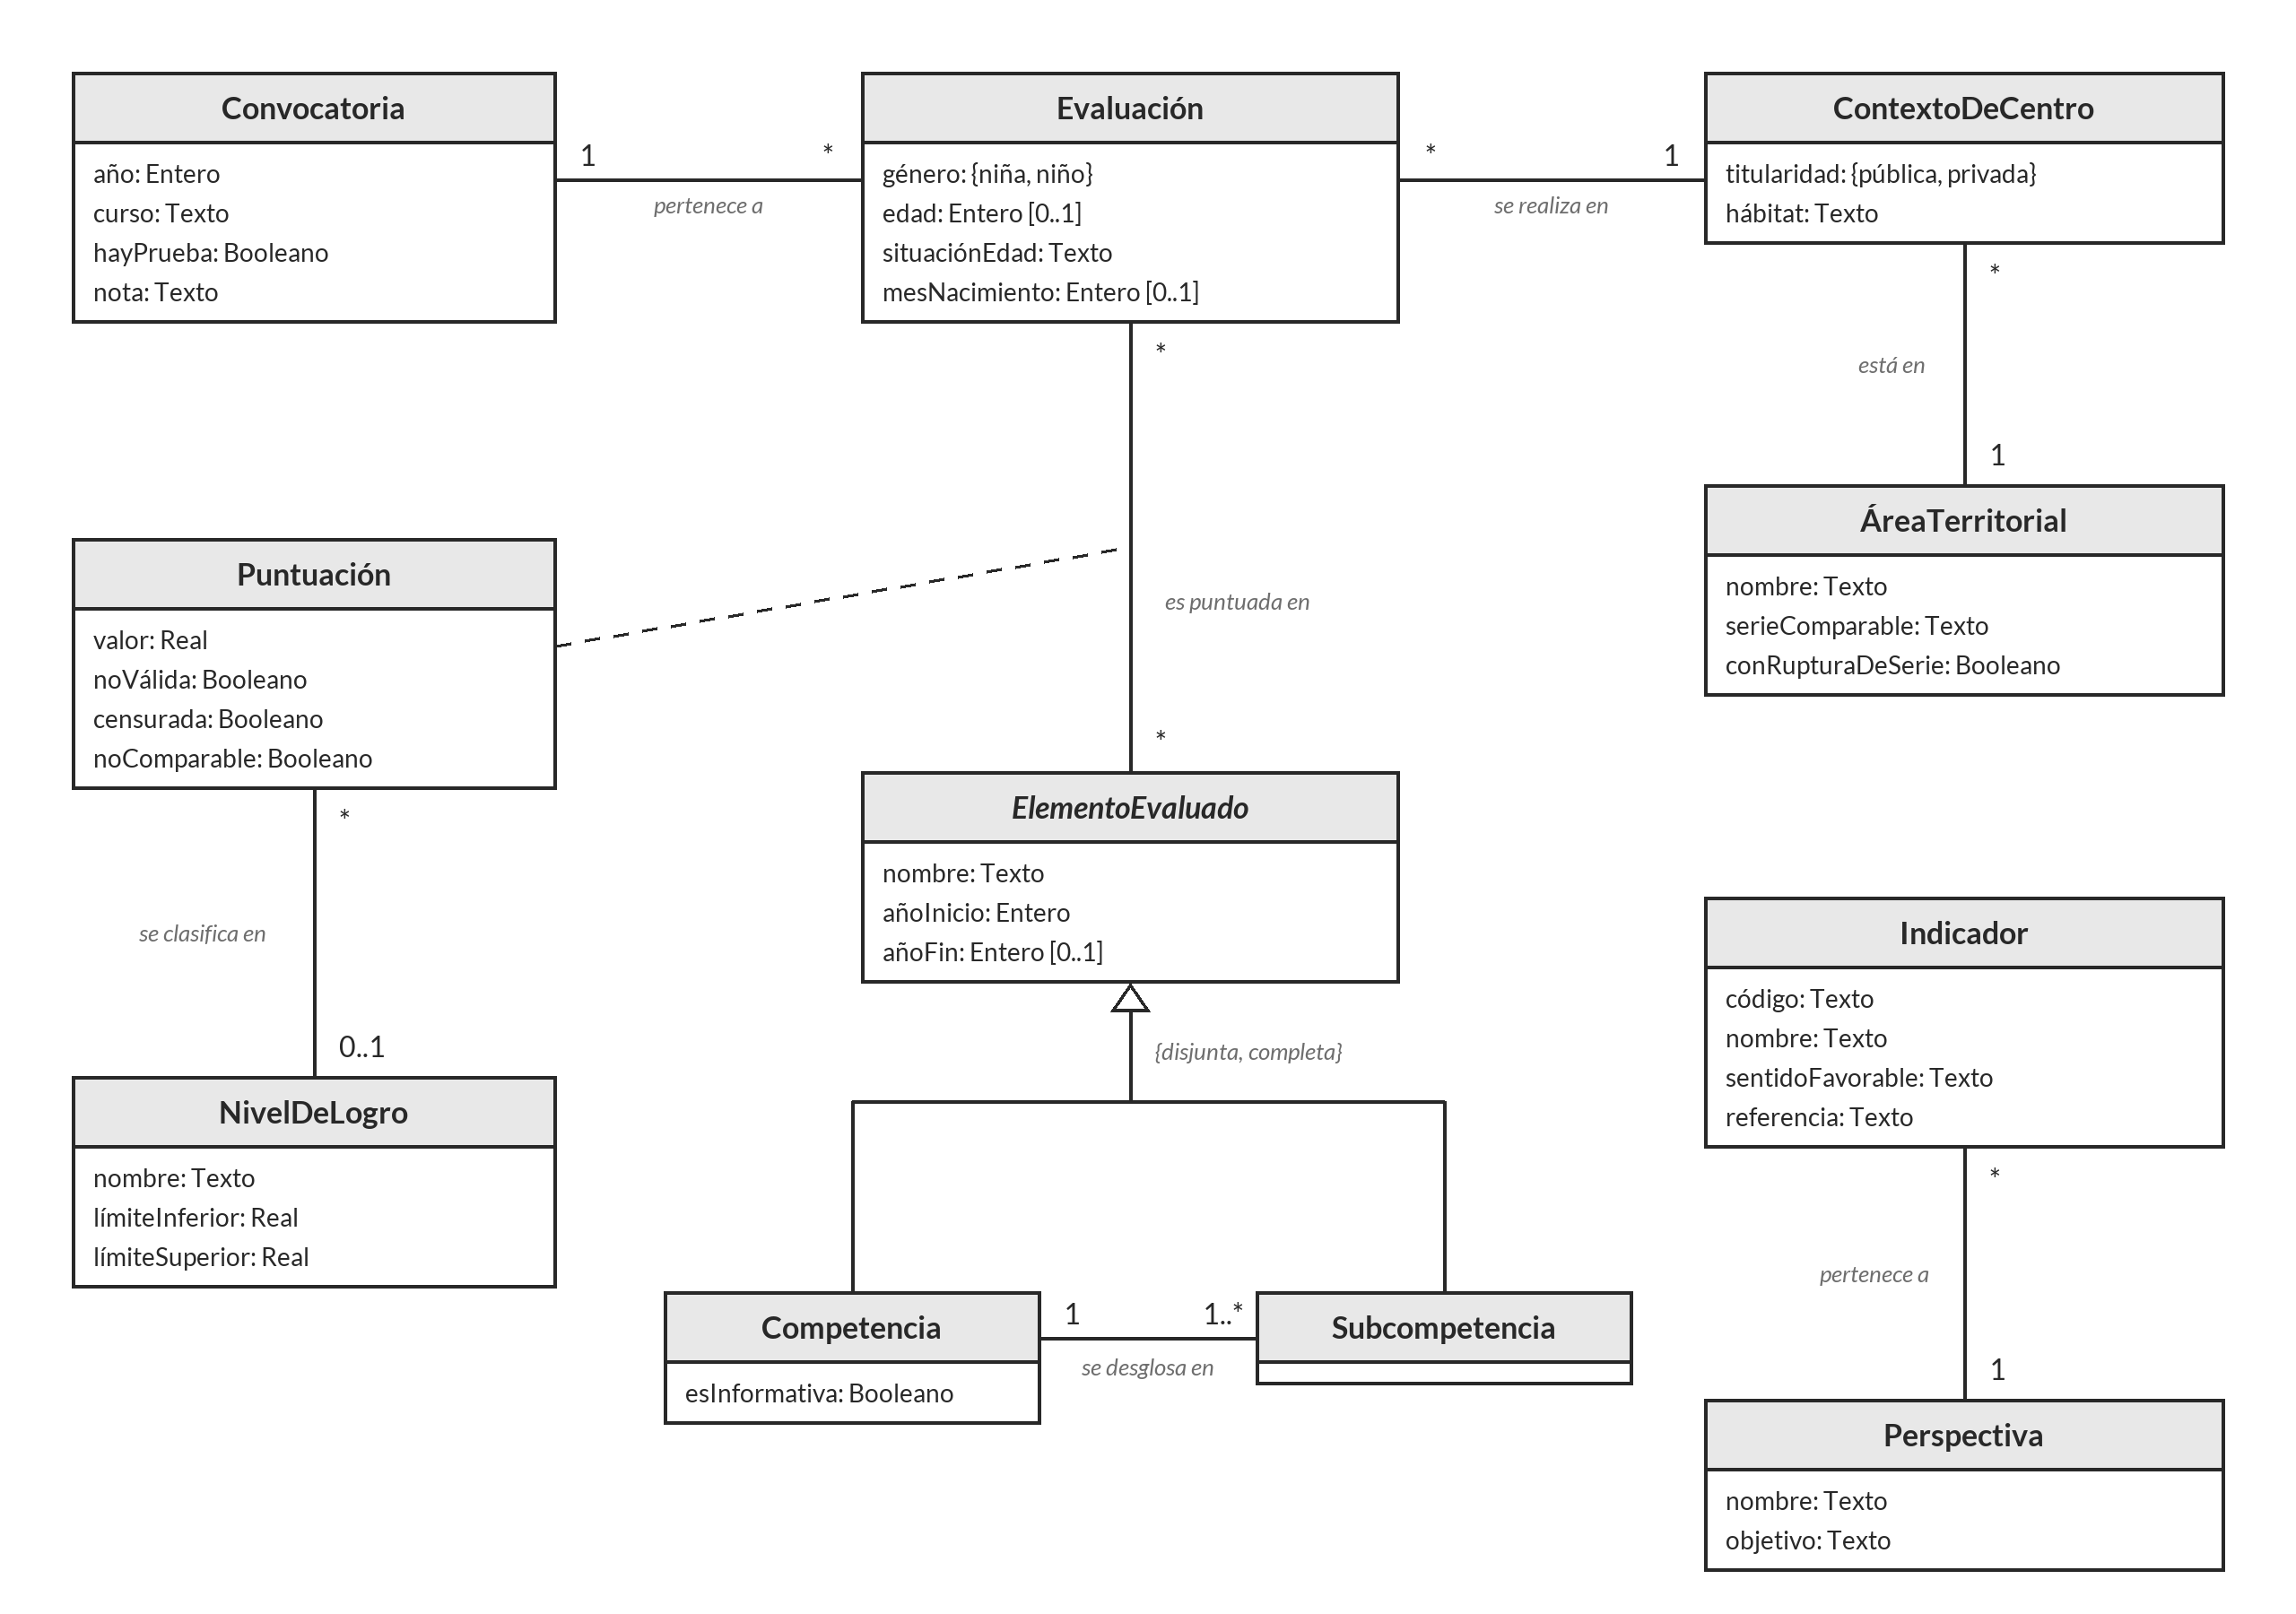
\includegraphics[width=\textwidth]{imagenes/especificacion/modelo_conceptual.png}
\caption{Modelo conceptual (diagrama de clases UML).}
\label{fig:modelo_conceptual}
\end{figure}

La clase central es \textit{Evaluación}, que representa la participación anónima de un alumno en una convocatoria. El conjunto de datos no tiene un identificador estable del alumnado ni el código del centro, así que el modelo no incluye las clases alumno ni centro. Cada evaluación se asocia a un \textit{ContextoDeCentro}, definido por el área territorial, la titularidad y el hábitat, que es lo que el cuadro de mando puede comparar (Sección~\ref{sec:preguntas}).

Lo que se evalúa es un \textit{ElementoEvaluado}, que puede ser una competencia, como la lengua catalana, o una de sus subcompetencias, como la comprensión lectora. Cada elemento tiene un periodo de vigencia, porque algunas subcompetencias aparecen o desaparecen entre convocatorias. La \textit{Puntuación} es una clase asociativa entre la evaluación y el elemento evaluado: guarda el valor y las marcas de calidad que asigna la depuración (RF04). Las puntuaciones de las competencias se clasifican además en un \textit{NivelDeLogro} (RF12).

\textit{Indicador} y \textit{Perspectiva} representan el catálogo del CMI (Tabla~\ref{tab:kpis}). Los indicadores no guardan ningún valor: se calculan a partir de las puntuaciones cada vez que el usuario consulta un panel o cambia un filtro.

\subsection{Restricciones de integridad}
\label{sec:restricciones}
El diagrama no puede expresar algunas condiciones, que se recogen como restricciones de integridad en la Tabla~\ref{tab:restricciones}.

\begin{table}[H]
\centering
\small
\renewcommand{\arraystretch}{1.1}
\begin{tabularx}{\textwidth}{@{} p{1.1cm} X @{}}
\toprule
\textbf{ID} & \textbf{Restricción} \\ \midrule
RI1 & Claves: una convocatoria se identifica por el año; un área territorial, un elemento evaluado, un nivel de logro y una perspectiva, por el nombre; un indicador, por el código; y un contexto de centro, por la combinación de área, titularidad y hábitat. \\ \addlinespace
RI2 & Una evaluación solo tiene puntuaciones de elementos vigentes en su convocatoria, es decir, con un año de inicio anterior o igual al de la convocatoria y sin año de fin o con uno posterior o igual. \\ \addlinespace
RI3 & Una puntuación tiene nivel de logro si y solo si es de una competencia. Ese nivel es el único cuyo intervalo contiene el valor de la puntuación. \\ \addlinespace
RI4 & Los intervalos de los niveles de logro no se solapan y entre todos cubren de 0 a 100. Cada intervalo incluye su límite inferior y excluye el superior, salvo el del nivel más alto, que incluye el 100. \\ \addlinespace
RI5 & Una convocatoria sin prueba (2020) no tiene evaluaciones. \\ \addlinespace
RI6 & La edad de una evaluación, si se conoce, está entre 10 y 14 años. \\ \addlinespace
RI7 & El valor de una puntuación está entre 0 y 100. \\ \bottomrule
\end{tabularx}
\caption{Restricciones de integridad del modelo conceptual.}
\label{tab:restricciones}
\end{table}

Las restricciones RI2, RI3 y RI5 se escriben además en OCL (\textit{Object Constraint Language}) \cite{omg_ocl24}, el lenguaje de restricciones de UML. Son las que relacionan varias clases, y en ellas el lenguaje natural deja más margen a la interpretación. Las claves, los intervalos de los niveles y los rangos de valores (RI1, RI4, RI6 y RI7) se quedan en lenguaje natural, porque formalizarlos alargaría el capítulo sin aclarar nada. Las expresiones usan los nombres del diagrama, con sus tildes, y recorren cada asociación con el nombre de la clase de destino con la inicial en minúscula, que es el nombre de rol que OCL asigna cuando el diagrama no indica otro.

RI2 se define sobre la puntuación, porque desde ella se llega a los dos extremos de la asociación a la que pertenece: la evaluación, que da el año de la convocatoria, y el elemento evaluado, que da el periodo de vigencia.

\par\vspace{2ex}\noindent\begin{minipage}{\textwidth}\small\setstretch{1.0}
\begin{verbatim}
context Puntuación inv elementoVigente:
  let añoConvocatoria = self.evaluación.convocatoria.año in
  self.elementoEvaluado.añoInicio <= añoConvocatoria and
  (self.elementoEvaluado.añoFin->isEmpty() or
   self.elementoEvaluado.añoFin >= añoConvocatoria)
\end{verbatim}
\end{minipage}\par\vspace{2.5ex}

RI3 se divide en dos invariantes. El primero exige que una puntuación tenga nivel de logro exactamente cuando su elemento evaluado es una competencia. El segundo exige que el valor esté dentro del intervalo de ese nivel, con los límites que fija RI4; como los intervalos no se solapan, ese nivel es único.

\par\vspace{2ex}\noindent\begin{minipage}{\textwidth}\small\setstretch{1.0}
\begin{verbatim}
context Puntuación inv nivelSoloEnCompetencias:
  self.nivelDeLogro->notEmpty() =
    self.elementoEvaluado.oclIsKindOf(Competencia)

context Puntuación inv nivelSegúnValor:
  self.nivelDeLogro->notEmpty() implies
    (self.nivelDeLogro.límiteInferior <= self.valor and
     (self.valor < self.nivelDeLogro.límiteSuperior or
      self.nivelDeLogro.límiteSuperior = 100))
\end{verbatim}
\end{minipage}\par\vspace{2.5ex}

RI5 se define sobre la convocatoria: si no hubo prueba, el conjunto de sus evaluaciones está vacío.

\par\vspace{2ex}\noindent\begin{minipage}{\textwidth}\small\setstretch{1.0}
\begin{verbatim}
context Convocatoria inv sinPruebaSinEvaluaciones:
  not self.hayPrueba implies self.evaluación->isEmpty()
\end{verbatim}
\end{minipage}\par\vspace{2.5ex}

\section{Arquitectura general}
\label{sec:arquitectura}
La Figura~\ref{fig:arquitectura} muestra el recorrido de los datos desde el fichero publicado hasta los paneles. El sistema es una cadena de etapas en la que cada una usa el resultado de la anterior:
\begin{enumerate}
    \item \textbf{Fuente.} El fichero CSV del Portal de Datos Abiertos, que se usa tal como se publica \cite{transparencia_catalunya_2024}.
    \item \textbf{ETL.} Power Query lee el fichero, comprueba que cumple las reglas de la auditoría, unifica los códigos, corrige los errores estructurales y marca la calidad de cada puntuación (RF01--RF05).
    \item \textbf{Modelo dimensional.} Los datos depurados se cargan en el motor en memoria de Power BI, en un esquema en estrella con dos tablas de hechos y seis dimensiones (Sección~\ref{sec:modelo_dimensional}).
    \item \textbf{Lógica analítica.} Las medidas DAX calculan los 12 KPIs, su estado y la regla de las 30 puntuaciones según los filtros activos en cada momento (RF11, RF13, RF14).
    \item \textbf{Interfaz.} El informe de Power BI contiene los tres paneles, uno por perfil (RF16--RF18), con los filtros sincronizados entre ellos (RF10).
\end{enumerate}

\begin{figure}[H]
\centering
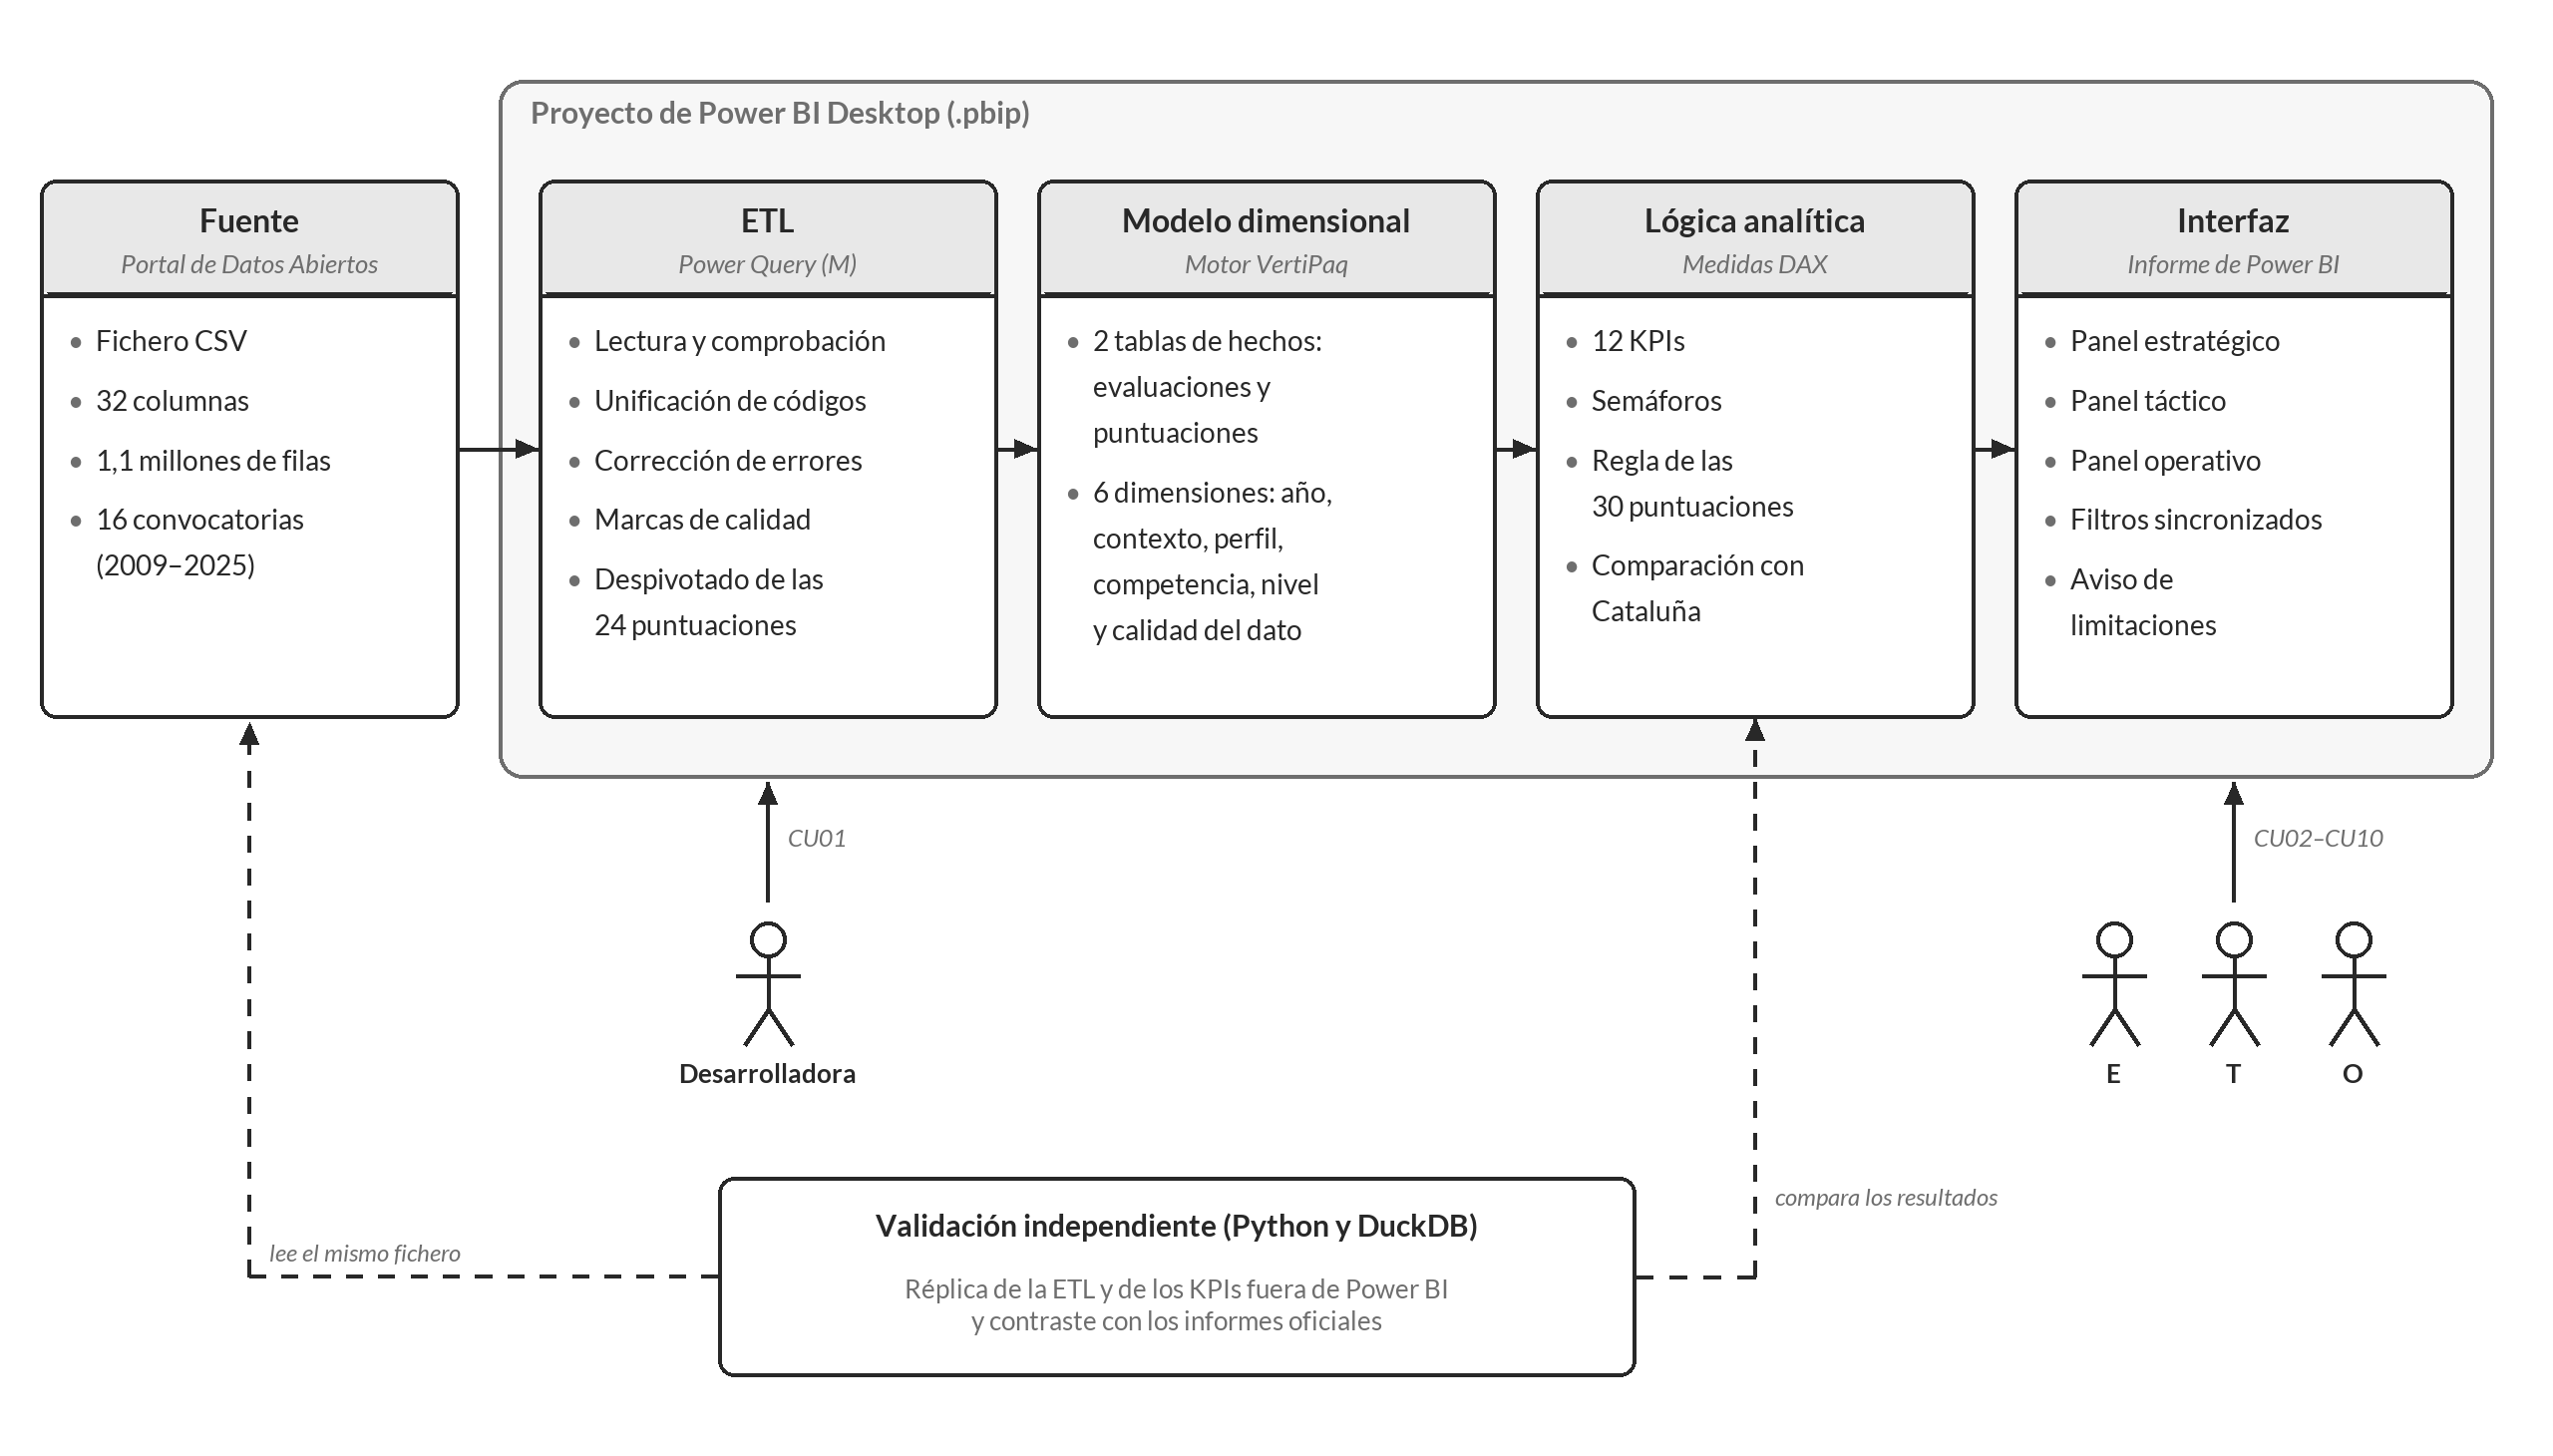
\includegraphics[width=\textwidth]{imagenes/especificacion/arquitectura.png}
\caption{Arquitectura general del sistema.}
\label{fig:arquitectura}
\end{figure}

Las etapas de la ETL a la interfaz forman un único proyecto de Power BI Desktop en formato \texttt{.pbip}, que guarda cada parte como texto y se versiona en Git (RNF10). Todo funciona con la versión gratuita de la herramienta (RNF11). La figura sitúa también los casos de uso: la desarrolladora actúa sobre la carga (CU01) y los tres perfiles, sobre los paneles (CU02--CU10).

Fuera de Power BI hay una validación independiente escrita en Python con DuckDB. Lee el mismo fichero, repite la depuración y el cálculo de los KPIs y compara sus resultados con los del modelo y con los informes oficiales \cite{csase_resultats}. Así se comprueba la exactitud de los cálculos (RNF06) con un método distinto al que se quiere validar (Sección~\ref{sec:validacion}).

\section{Especificación de los requisitos no funcionales}
\label{sec:rnf_volere}
Los requisitos no funcionales de la Tabla~\ref{tab:rnf} se especifican con la plantilla Volere \cite{robertson2012mastering}, que describe cada requisito en una ficha. Se usa una versión reducida, con los cinco campos que hacen falta en este proyecto: el tipo de requisito, la descripción, la justificación, el criterio de aceptación y el método de evaluación. El tipo es la característica de calidad de la norma ISO/IEC 25010 \cite{iso25010_2011} a la que pertenece el requisito, con la subcaracterística entre paréntesis. El criterio de aceptación fija el valor que debe alcanzarse y es el mismo de la Tabla~\ref{tab:rnf}. El método de evaluación indica cómo se comprobará, de acuerdo con los métodos de validación de la Sección~\ref{sec:validacion}.

La plantilla se aplica solo a los requisitos no funcionales (Tablas~\ref{tab:rnf01} a \ref{tab:rnf11}). Los funcionales se especifican con los casos de uso de la Sección~\ref{sec:casos_uso}.

\begin{table}[H]
\centering
\small
\setstretch{1.0}\renewcommand{\arraystretch}{1.0}\setlength{\defaultaddspace}{3pt}
\begin{tabularx}{\textwidth}{@{} >{\raggedright\arraybackslash}p{3.4cm} X @{}}
\toprule
\textbf{RNF01} & \textbf{Tiempo de respuesta} \\ \midrule
Requisito de & Eficiencia de desempeño (comportamiento temporal). \\ \addlinespace
Descripción & Los paneles responden con rapidez cuando el usuario aplica un filtro o cambia de panel, con todas las convocatorias cargadas. \\ \addlinespace
Justificación & El modelo contiene 1,1 millones de evaluaciones y 17,7 millones de puntuaciones. Si cada filtro tarda en aplicarse, el usuario deja de explorar los datos y se queda con la vista inicial. \\ \addlinespace
Criterio de aceptación & Cada interacción tarda menos de 3 s desde la acción del usuario hasta que se actualiza el último elemento visual del panel. \\ \addlinespace
Método de evaluación & Medición con el analizador de rendimiento de Power BI Desktop en el equipo de desarrollo: se cambia cada filtro y se pasa de un panel a otro en los tres paneles, tres veces, y se toma el peor tiempo. Las consultas más lentas se analizan con DAX Studio \cite{dax_studio}. \\ \bottomrule
\end{tabularx}
\caption{Ficha Volere del requisito RNF01.}
\label{tab:rnf01}
\end{table}

\begin{table}[!htbp]
\centering
\small
\setstretch{1.0}\renewcommand{\arraystretch}{1.0}\setlength{\defaultaddspace}{3pt}
\begin{tabularx}{\textwidth}{@{} >{\raggedright\arraybackslash}p{3.4cm} X @{}}
\toprule
\textbf{RNF02} & \textbf{Facilidad de uso} \\ \midrule
Requisito de & Usabilidad (capacidad de aprendizaje y operabilidad). \\ \addlinespace
Descripción & Una persona sin formación técnica entiende los paneles y encuentra en ellos la información que busca sin ayuda. \\ \addlinespace
Justificación & Los tres perfiles son responsables educativos, inspectores y directores de centro, no analistas de datos. Un cuadro de mando que exige formación previa se deja de usar. \\ \addlinespace
Criterio de aceptación & Puntuación media igual o superior a 68 en el cuestionario SUS \cite{brooke1996sus}, con al menos 5 participantes. \\ \addlinespace
Método de evaluación & Prueba con usuarios de perfiles representativos: tareas guiadas en los tres paneles y cuestionario SUS al terminar. Se complementa con una evaluación heurística \cite{nielsen1993usability}. \\ \bottomrule
\end{tabularx}
\caption{Ficha Volere del requisito RNF02.}
\label{tab:rnf02}
\end{table}

\begin{table}[!htbp]
\centering
\small
\setstretch{1.0}\renewcommand{\arraystretch}{1.0}\setlength{\defaultaddspace}{3pt}
\begin{tabularx}{\textwidth}{@{} >{\raggedright\arraybackslash}p{3.4cm} X @{}}
\toprule
\textbf{RNF03} & \textbf{Panel en una sola pantalla} \\ \midrule
Requisito de & Usabilidad (operabilidad). \\ \addlinespace
Descripción & Cada panel muestra todo su contenido en una pantalla, sin desplazamiento vertical ni horizontal. \\ \addlinespace
Justificación & Un cuadro de mando se lee de un vistazo \cite{few2006information}. Lo que queda fuera de la pantalla no se compara con lo demás y obliga al usuario a recordarlo. \\ \addlinespace
Criterio de aceptación & Las tres páginas del informe tienen un lienzo de 1280 $\times$ 720 píxeles, ningún elemento visual sobresale de él y la página no tiene barras de desplazamiento. \\ \addlinespace
Método de evaluación & Comprobación del tamaño de cada página y de la posición de cada elemento en los ficheros del informe, e inspección de los tres paneles en Power BI Desktop con la vista ajustada a la página. \\ \bottomrule
\end{tabularx}
\caption{Ficha Volere del requisito RNF03.}
\label{tab:rnf03}
\end{table}

\begin{table}[!htbp]
\centering
\small
\setstretch{1.0}\renewcommand{\arraystretch}{1.0}\setlength{\defaultaddspace}{3pt}
\begin{tabularx}{\textwidth}{@{} >{\raggedright\arraybackslash}p{3.4cm} X @{}}
\toprule
\textbf{RNF04} & \textbf{Idioma y terminología} \\ \midrule
Requisito de & Usabilidad (capacidad para reconocer su adecuación). \\ \addlinespace
Descripción & Toda la interfaz está en castellano y nombra las competencias y las áreas territoriales como los informes oficiales. \\ \addlinespace
Justificación & El usuario contrasta el cuadro de mando con los informes del Consell Superior d'Avaluació \cite{csase_resultats}. Si los nombres no coinciden, duda de que las cifras se refieran a lo mismo. \\ \addlinespace
Criterio de aceptación & Ningún título, etiqueta, aviso o descripción emergente está en otro idioma. Los nombres de las competencias son la traducción al castellano de los oficiales, y los de las áreas territoriales, que son nombres propios, se mantienen como en la fuente. \\ \addlinespace
Método de evaluación & Revisión de todos los textos de los tres paneles con una lista de comprobación y contraste de los nombres con los de los informes oficiales. \\ \bottomrule
\end{tabularx}
\caption{Ficha Volere del requisito RNF04.}
\label{tab:rnf04}
\end{table}

\begin{table}[!htbp]
\centering
\small
\setstretch{1.0}\renewcommand{\arraystretch}{1.0}\setlength{\defaultaddspace}{3pt}
\begin{tabularx}{\textwidth}{@{} >{\raggedright\arraybackslash}p{3.4cm} X @{}}
\toprule
\textbf{RNF05} & \textbf{Accesibilidad visual} \\ \midrule
Requisito de & Usabilidad (accesibilidad). \\ \addlinespace
Descripción & Los paneles se pueden leer con daltonismo o con baja visión. \\ \addlinespace
Justificación & El estado de los KPIs y las series de los gráficos se distinguen por el color. Quien no diferencia el rojo del verde, o no lee un texto con poco contraste, perdería esa información. \\ \addlinespace
Criterio de aceptación & Contraste entre el texto y su fondo de al menos 4,5:1 (nivel AA de WCAG 2.1 \cite{w3c_wcag21}) y paletas cuyos colores se distinguen con deuteranopía y con protanopía. \\ \addlinespace
Método de evaluación & Cálculo de la razón de contraste de cada combinación de color de texto y de fondo con la fórmula de WCAG 2.1, y revisión de capturas de los tres paneles con un simulador de daltonismo. \\ \bottomrule
\end{tabularx}
\caption{Ficha Volere del requisito RNF05.}
\label{tab:rnf05}
\end{table}

\begin{table}[!htbp]
\centering
\small
\setstretch{1.0}\renewcommand{\arraystretch}{1.0}\setlength{\defaultaddspace}{3pt}
\begin{tabularx}{\textwidth}{@{} >{\raggedright\arraybackslash}p{3.4cm} X @{}}
\toprule
\textbf{RNF06} & \textbf{Exactitud de los resultados} \\ \midrule
Requisito de & Adecuación funcional (corrección funcional). \\ \addlinespace
Descripción & Los indicadores se calculan con exactitud a partir de los datos publicados. \\ \addlinespace
Justificación & Las decisiones se toman a partir de estas cifras. Los informes oficiales son la única referencia externa disponible, así que una diferencia con ellos apunta a un error en la ETL o en las medidas. \\ \addlinespace
Criterio de aceptación & La puntuación media de Cataluña de cada competencia y convocatoria difiere menos de 0,5 puntos de la publicada en los informes oficiales \cite{csase_resultats}. \\ \addlinespace
Método de evaluación & Validación independiente en Python (Sección~\ref{sec:arquitectura}): repite la ETL y el cálculo de los KPIs, compara cada media con la oficial y sirve de referencia para contrastar los valores que muestra Power BI. \\ \bottomrule
\end{tabularx}
\caption{Ficha Volere del requisito RNF06.}
\label{tab:rnf06}
\end{table}

\begin{table}[!htbp]
\centering
\small
\setstretch{1.0}\renewcommand{\arraystretch}{1.0}\setlength{\defaultaddspace}{3pt}
\begin{tabularx}{\textwidth}{@{} >{\raggedright\arraybackslash}p{3.4cm} X @{}}
\toprule
\textbf{RNF07} & \textbf{Trazabilidad de la limpieza} \\ \midrule
Requisito de & Adecuación funcional (corrección funcional). \\ \addlinespace
Descripción & Cada regla de limpieza está documentada y su efecto sobre los datos se puede reproducir. \\ \addlinespace
Justificación & La limpieza cambia los datos publicados; por ejemplo, recoloca las columnas de puntuación rotadas. Quien revise el cuadro de mando debe poder saber qué se cambió y comprobarlo. \\ \addlinespace
Criterio de aceptación & Todas las reglas que aplica la ETL figuran en el informe de calidad de los datos con su identificador y con las filas afectadas, y la validación independiente obtiene los mismos recuentos. \\ \addlinespace
Método de evaluación & Revisión cruzada de las reglas de la ETL y del informe de calidad, y ejecución de las pruebas de integridad de la validación independiente, que repite la limpieza y comprueba los recuentos. \\ \bottomrule
\end{tabularx}
\caption{Ficha Volere del requisito RNF07.}
\label{tab:rnf07}
\end{table}

\begin{table}[!htbp]
\centering
\small
\setstretch{1.0}\renewcommand{\arraystretch}{1.0}\setlength{\defaultaddspace}{3pt}
\begin{tabularx}{\textwidth}{@{} >{\raggedright\arraybackslash}p{3.4cm} X @{}}
\toprule
\textbf{RNF08} & \textbf{Protección de datos} \\ \midrule
Requisito de & Seguridad (confidencialidad). \\ \addlinespace
Descripción & El sistema trabaja solo con datos anonimizados y no expone ningún identificador del alumnado, como exige el RGPD. \\ \addlinespace
Justificación & Los datos son de menores. El fichero publicado es anónimo, pero incluye un código de alumno que el cuadro de mando no necesita para calcular ningún indicador. \\ \addlinespace
Criterio de aceptación & Ninguna tabla del modelo contiene el código de alumno ni otro campo identificador, y ningún panel muestra registros individuales. \\ \addlinespace
Método de evaluación & Inspección de las columnas del modelo en los ficheros del proyecto y revisión de los elementos visuales de los tres paneles. \\ \bottomrule
\end{tabularx}
\caption{Ficha Volere del requisito RNF08.}
\label{tab:rnf08}
\end{table}

\begin{table}[!htbp]
\centering
\small
\setstretch{1.0}\renewcommand{\arraystretch}{1.0}\setlength{\defaultaddspace}{3pt}
\begin{tabularx}{\textwidth}{@{} >{\raggedright\arraybackslash}p{3.4cm} X @{}}
\toprule
\textbf{RNF09} & \textbf{Incorporación de convocatorias} \\ \midrule
Requisito de & Mantenibilidad (capacidad para ser modificado). \\ \addlinespace
Descripción & Una convocatoria nueva se incorpora sin rediseñar el modelo. \\ \addlinespace
Justificación & El Portal de Datos Abiertos publica una convocatoria cada año. Si cada una obligara a cambiar tablas o medidas, el cuadro de mando quedaría desactualizado al terminar el TFG. \\ \addlinespace
Criterio de aceptación & Para cargar una convocatoria nueva basta con sustituir el fichero de origen y actualizar. Como mucho cambian parámetros documentados, y no se modifica ninguna tabla, relación ni medida. \\ \addlinespace
Método de evaluación & Prueba de carga en dos pasos: primero con un fichero sin la última convocatoria y después con el fichero completo. Se comprueba que la convocatoria aparece en los paneles y que el número de registros de cada convocatoria coincide con el del fichero. \\ \bottomrule
\end{tabularx}
\caption{Ficha Volere del requisito RNF09.}
\label{tab:rnf09}
\end{table}

\begin{table}[!htbp]
\centering
\small
\setstretch{1.0}\renewcommand{\arraystretch}{1.0}\setlength{\defaultaddspace}{3pt}
\begin{tabularx}{\textwidth}{@{} >{\raggedright\arraybackslash}p{3.4cm} X @{}}
\toprule
\textbf{RNF10} & \textbf{Artefactos en texto y versionados} \\ \midrule
Requisito de & Mantenibilidad (analizabilidad). \\ \addlinespace
Descripción & Todos los artefactos del proyecto se guardan en formato de texto y bajo control de versiones. \\ \addlinespace
Justificación & Un fichero binario de Power BI no deja ver qué ha cambiado entre dos versiones. Con ficheros de texto, cada cambio en la ETL, en el modelo o en las medidas queda registrado y se puede revisar o deshacer. \\ \addlinespace
Criterio de aceptación & El proyecto de Power BI está en formato \texttt{.pbip} y el repositorio de Git contiene el modelo, las consultas, las medidas, el informe y los scripts como ficheros de texto, sin ningún fichero \texttt{.pbix}. \\ \addlinespace
Método de evaluación & Inspección del contenido del repositorio y de su historial de cambios. \\ \bottomrule
\end{tabularx}
\caption{Ficha Volere del requisito RNF10.}
\label{tab:rnf10}
\end{table}

\begin{table}[!htbp]
\centering
\small
\setstretch{1.0}\renewcommand{\arraystretch}{1.0}\setlength{\defaultaddspace}{3pt}
\begin{tabularx}{\textwidth}{@{} >{\raggedright\arraybackslash}p{3.4cm} X @{}}
\toprule
\textbf{RNF11} & \textbf{Uso sin licencias de pago} \\ \midrule
Requisito de & Portabilidad (capacidad para ser instalado). \\ \addlinespace
Descripción & El cuadro de mando funciona sin licencias de pago. \\ \addlinespace
Justificación & No se puede dar por hecho que los centros y la inspección tengan licencias de Power BI. Si el uso dependiera de ellas, parte de los destinatarios no podría abrir el cuadro de mando. \\ \addlinespace
Criterio de aceptación & El proyecto se abre, se actualiza y se usa completo con Power BI Desktop, que es gratuito \cite{ms_powerbi_pricing}, sin iniciar sesión y sin elementos visuales ni funciones de pago. \\ \addlinespace
Método de evaluación & Prueba en un equipo distinto del de desarrollo, con Power BI Desktop recién instalado y sin cuenta: se abre el proyecto, se actualizan los datos y se recorren los tres paneles. \\ \bottomrule
\end{tabularx}
\caption{Ficha Volere del requisito RNF11.}
\label{tab:rnf11}
\end{table}

\FloatBarrier
\section{Historias de usuario}
\label{sec:historias}
Las historias de usuario recogen los requisitos como necesidades concretas de quien usa el sistema y forman el \textit{backlog} del desarrollo (Sección~\ref{sec:metodologia}). Siguen el formato \guillemotleft{}Como [perfil], quiero [acción] para [objetivo]\guillemotright{} y cada una tiene criterios de aceptación, que permiten decidir en la revisión de cada \textit{sprint} si la historia está terminada. Un caso de uso describe una interacción completa con el sistema, y una historia, una sola necesidad, así que un mismo caso de uso puede dar lugar a varias historias.

La Tabla~\ref{tab:historias} agrupa las historias por perfil. La columna de trazabilidad indica el caso de uso, los requisitos y la prioridad. La prioridad sigue el alcance de la Tabla~\ref{tab:alcance}: las historias imprescindibles forman el alcance mínimo y la única opcional (HU15) corresponde a una de las extensiones.

{\small\setstretch{1.0}\renewcommand{\arraystretch}{1.15}
\begin{longtable}{@{} p{1cm} p{10.6cm} >{\raggedright\arraybackslash}p{2.7cm} @{}}
\toprule
\textbf{ID} & \textbf{Historia y criterios de aceptación} & \textbf{Trazabilidad} \\ \midrule
\endfirsthead
\toprule
\textbf{ID} & \textbf{Historia y criterios de aceptación} & \textbf{Trazabilidad} \\ \midrule
\endhead
\bottomrule
\caption{Historias de usuario.}\label{tab:historias}
\endlastfoot
\multicolumn{3}{@{}l}{\textit{Perfil estratégico (Departamento de Educación)}} \\
HU01 & \textit{Como responsable del Departamento de Educación, quiero ver de un vistazo la puntuación media de Cataluña y el porcentaje de alumnado con nivel bajo para saber si las competencias básicas mejoran.}\newline \textbullet{} Al abrir el panel aparecen K01 y K03 de la última convocatoria.\newline \textbullet{} La variación respecto a la convocatoria anterior muestra su estado: favorable, neutro o desfavorable.\newline \textbullet{} Las medias de Cataluña difieren menos de 0,5 puntos de las oficiales. & CU02\newline RF11, RF13, RF16\newline Imprescindible \\ \addlinespace
HU02 & \textit{Como responsable del Departamento de Educación, quiero ver la evolución de cada competencia en todas las convocatorias para detectar tendencias.}\newline \textbullet{} El gráfico muestra de 2009 a 2025 aunque se filtre un año.\newline \textbullet{} 2020 aparece como un hueco señalado.\newline \textbullet{} El aviso sobre la comparabilidad entre convocatorias está a la vista. & CU06\newline RF08, RF15\newline Imprescindible \\ \addlinespace
HU03 & \textit{Como responsable del Departamento de Educación, quiero saber qué competencias empeoran respecto a la convocatoria anterior para decidir dónde intervenir.}\newline \textbullet{} Una tabla muestra la variación (K10) de cada competencia.\newline \textbullet{} Una tarjeta indica el porcentaje de competencias que mejoran (K12).\newline \textbullet{} En la primera convocatoria la variación queda en blanco. & CU02\newline RF11, RF16\newline Imprescindible \\ \addlinespace
\multicolumn{3}{@{}l}{\textit{Perfil táctico (inspección y coordinación territorial)}} \\
HU04 & \textit{Como inspector o inspectora, quiero comparar cada área territorial con la media de Cataluña para detectar las que se alejan.}\newline \textbullet{} Un gráfico muestra la desviación (K07) de todas las áreas.\newline \textbullet{} Al seleccionar un área se siguen viendo las demás, y su posición y su estado aparecen en las tarjetas. & CU03, CU07\newline RF09, RF17\newline Imprescindible \\ \addlinespace
HU05 & \textit{Como inspector o inspectora, quiero conocer las brechas de género, titularidad y hábitat para detectar problemas de equidad.}\newline \textbullet{} El panel muestra K04, K05 y K08 con el filtro activo.\newline \textbullet{} El signo de cada brecha indica a favor de qué grupo es.\newline \textbullet{} Una brecha calculada sobre menos de 30 puntuaciones queda en blanco. & CU03\newline RF11, RF14, RF17\newline Imprescindible \\ \addlinespace
HU06 & \textit{Como inspector o inspectora, quiero ver la posición de mi área entre todas para decidir dónde priorizar el refuerzo.}\newline \textbullet{} Al seleccionar un área aparece su posición (K09) sobre el total de áreas.\newline \textbullet{} Sin área seleccionada, la posición queda en blanco. & CU03\newline RF17\newline Imprescindible \\ \addlinespace
HU07 & \textit{Como inspector o inspectora, quiero seguir la evolución de las áreas aunque haya cambiado la organización territorial para comparar convocatorias.}\newline \textbullet{} Las áreas se agrupan en series comparables entre convocatorias.\newline \textbullet{} Las áreas afectadas por la reorganización de 2024 están señaladas. & CU06\newline RF08, RF15\newline Imprescindible \\ \addlinespace
\multicolumn{3}{@{}l}{\textit{Perfil operativo (dirección de centro)}} \\
HU08 & \textit{Como director o directora de un centro, quiero definir el contexto de mi centro para compararme con centros parecidos.}\newline \textbullet{} El panel tiene filtros de área, titularidad y hábitat.\newline \textbullet{} Los indicadores se actualizan en menos de 3 segundos.\newline \textbullet{} Si el contexto tiene menos de 30 puntuaciones, los indicadores quedan en blanco. & CU04, CU05\newline RF06, RF14, RF18\newline Imprescindible \\ \addlinespace
HU09 & \textit{Como director o directora de un centro, quiero ver la desviación de mi contexto respecto a Cataluña para saber si estamos por encima o por debajo.}\newline \textbullet{} Una tarjeta muestra la desviación (K07) con su estado.\newline \textbullet{} La media de Cataluña aparece al lado como referencia. & CU07\newline RF09, RF13\newline Imprescindible \\ \addlinespace
HU10 & \textit{Como director o directora de un centro, quiero ver la puntuación de cada subcompetencia para saber en qué aspectos concretos hay más carencias.}\newline \textbullet{} Las subcompetencias (K02) se agrupan por competencia.\newline \textbullet{} Al seleccionar una competencia solo se ven sus subcompetencias. & CU08\newline RF07\newline Imprescindible \\ \addlinespace
HU11 & \textit{Como director o directora de un centro, quiero ver cómo se reparte el alumnado por niveles de logro para estimar cuántos alumnos necesitan refuerzo.}\newline \textbullet{} Cada competencia muestra los cuatro niveles y entre todos suman el 100\%.\newline \textbullet{} Las puntuaciones censuradas o de convocatorias con niveles no comparables no se cuentan. & CU09\newline RF04, RF12\newline Imprescindible \\ \addlinespace
\multicolumn{3}{@{}l}{\textit{Comunes, de la desarrolladora y opcionales}} \\
HU12 & \textit{Como usuario del CMI, quiero que se mantenga la selección de año, competencia y área al cambiar de panel para no tener que repetir los filtros.}\newline \textbullet{} Al cambiar de panel, los filtros de año, competencia y área conservan su valor.\newline \textbullet{} Cada panel cabe en una pantalla sin desplazamiento. & CU05, CU10\newline RF10, RNF03\newline Imprescindible \\ \addlinespace
HU13 & \textit{Como desarrolladora, quiero incorporar una convocatoria nueva sustituyendo el fichero para no tener que rediseñar el modelo cada año.}\newline \textbullet{} La actualización solo requiere cambiar el fichero y, si acaso, parámetros documentados.\newline \textbullet{} El número de registros por convocatoria coincide con el del fichero. & CU01\newline RF01, RNF09\newline Imprescindible \\ \addlinespace
HU14 & \textit{Como desarrolladora, quiero que la carga se detenga cuando el fichero tenga algo no previsto para no publicar datos erróneos.}\newline \textbullet{} Una puntuación fuera de 0--100 o un código desconocido detienen la carga.\newline \textbullet{} El mensaje indica la regla incumplida.\newline \textbullet{} Se conservan los datos de la carga anterior. & CU01\newline RF02--RF05\newline Imprescindible \\ \addlinespace
HU15 & \textit{Como inspector o inspectora, quiero consultar el CMI desde el navegador y ver solo mi territorio para no tener que instalar Power BI Desktop.}\newline \textbullet{} El informe está publicado en Power BI Service.\newline \textbullet{} La seguridad a nivel de fila limita los datos al área del usuario. & Extensión\newline Tabla~\ref{tab:alcance}\newline Opcional \\ \addlinespace
\end{longtable}}

% ------------------------------------------
% CAPÍTULO 8: DISEÑO
% ------------------------------------------
\chapter{Diseño}
\label{cap:diseno}
% Nombres vinculantes: trabajo_en_curso/week2/DECISIONES.md, sección «Nombres».
El diseño describe cómo se construye el sistema especificado en el Capítulo~\ref{cap:especificacion}. Tiene un apartado por cada etapa de la arquitectura general (Sección~\ref{sec:arquitectura}): el modelo dimensional, la ETL, la lógica analítica y la interfaz. El modelo dimensional va primero porque la ETL se diseña para cargarlo. El último apartado describe la organización del repositorio, donde se guardan todos los ficheros del proyecto.

El capítulo recoge las decisiones de diseño y su justificación. El detalle completo está en cuatro documentos del repositorio (Sección~\ref{sec:organizacion_proyecto}): el informe de calidad de los datos, el documento del modelo con el diccionario de datos, las fichas de los KPIs y la guía de uso. Las cifras de filas y de resultados proceden del modelo implementado y se han comprobado con la validación independiente en Python.

\section{Diseño del modelo dimensional}
\label{sec:modelo_dimensional}
El modelo dimensional es la base de datos del sistema: las tablas que la ETL carga en Power BI y sobre las que se calculan los KPIs. Parte del modelo conceptual de la Sección~\ref{sec:modelo_conceptual}, que es el diseño conceptual del sistema, y de sus restricciones de integridad (Tabla~\ref{tab:restricciones}). El diseño sigue el método de Kimball \cite{kimball2013data}. Primero se traducen las clases a tablas de hechos y dimensiones. Después se fija la granularidad de cada tabla de hechos y se definen las dimensiones. Al final, las columnas se documentan en el diccionario de datos.

El subobjetivo SO3 preveía cuatro dimensiones: tiempo, alumno, contexto del centro y competencia. El diseño añade dos, el nivel de logro y la calidad del dato. Las restricciones RI3 y RI4 y el requisito RF04 obligan a guardar en cada puntuación su nivel y sus marcas de calidad, y como dimensiones se pueden filtrar igual que el resto.

\subsection{Diseño lógico: esquema en estrella}
\label{sec:diseno_logico}
El diseño lógico traduce el modelo conceptual a tablas. La Tabla~\ref{tab:correspondencia} indica en qué tabla acaba cada clase o asociación y cómo se traduce.

{\small\setstretch{1.0}\renewcommand{\arraystretch}{1.1}
\begin{longtable}{@{} >{\raggedright\arraybackslash}p{3.5cm} >{\raggedright\arraybackslash}p{3.6cm} p{7.2cm} @{}}
\toprule
\textbf{Modelo conceptual} & \textbf{Tabla} & \textbf{Traducción} \\ \midrule
\endfirsthead
\toprule
\textbf{Modelo conceptual} & \textbf{Tabla} & \textbf{Traducción} \\ \midrule
\endhead
\bottomrule
\caption{Correspondencia entre el modelo conceptual y el modelo dimensional.}\label{tab:correspondencia}
\endlastfoot
\textit{Evaluación} & \texttt{FactEvaluacion} y \texttt{DimPerfilAlumno} & Cada evaluación es una fila de hechos. Sus atributos (género, edad, situación de edad y mes de nacimiento) pasan a una dimensión con todas las combinaciones posibles. El código de alumno no se carga (RNF08). \\ \addlinespace
\textit{Puntuación} (clase asociativa) & \texttt{FactPuntuacion} & Cada puntuación no nula es una fila de hechos con las claves de su evaluación y de su elemento evaluado, el valor y las claves del nivel de logro y de la calidad. \\ \addlinespace
\textit{Convocatoria} & \texttt{DimAnio} & Una fila por año de 2009 a 2025, incluido 2020, que no tiene evaluaciones. \\ \addlinespace
\textit{ContextoDeCentro} y \textit{ÁreaTerritorial} & \texttt{DimContextoCentro} & Las dos clases se funden en una dimensión con todas las combinaciones de área, titularidad y hábitat. Los atributos del área (serie comparable y ruptura de serie) son columnas de esa dimensión. \\ \addlinespace
\textit{ElementoEvaluado}, \textit{Competencia}, \textit{Subcompetencia} y \guillemotleft{}se desglosa en\guillemotright{} & \texttt{DimCompetencia} & La jerarquía se aplana en una tabla con una fila por columna de puntuación del fichero (24). \texttt{EsGlobal} distingue las competencias de las subcompetencias y \texttt{Materia} agrupa cada subcompetencia en su competencia. \\ \addlinespace
\textit{NivelDeLogro} y \guillemotleft{}se clasifica en\guillemotright{} & \texttt{DimNivelLogro} & Los cuatro niveles más un miembro \guillemotleft{}No aplica\guillemotright{} que reciben las subcompetencias, de modo que la clave del nivel nunca es nula. \\ \addlinespace
Marcas de calidad de \textit{Puntuación} & \texttt{DimCalidadDato} & Las cuatro marcas se codifican en una sola clave, una máscara de 4 bits, y la dimensión enumera sus 16 combinaciones. \\ \addlinespace
\textit{Indicador} y \textit{Perspectiva} & Ninguna & Cada indicador es una medida DAX y cada perspectiva, una carpeta de medidas (Sección~\ref{sec:diseno_dax}). \\
\end{longtable}}

La traducción sigue tres criterios. El primero es fundir en la dimensión las clases que solo describen a otra. \textit{ÁreaTerritorial} solo se usa a través del contexto del centro, así que sus atributos se repiten en \texttt{DimContextoCentro} en lugar de formar una tabla encadenada. El esquema queda así en estrella y no en copo de nieve, que es la forma que recomienda Kimball para el análisis \cite{kimball2013data}. Lo mismo ocurre con la especialización de \textit{ElementoEvaluado}, que se convierte en un atributo.

El segundo criterio es que ninguna fila de hechos tenga una clave nula. Cada ausencia se representa con un miembro propio de la dimensión: el nivel \guillemotleft{}No aplica\guillemotright{}, el área \guillemotleft{}Desconocida\guillemotright{}, el hábitat \guillemotleft{}No fiable\guillemotright{} o la situación de edad \guillemotleft{}Desconocida\guillemotright{}. Así cualquier filtro sobre una dimensión cuenta todas las filas de hechos.

El tercero es usar claves deterministas. Cada clave se calcula con una fórmula a partir de los códigos del fichero; por ejemplo, la del contexto es $\mathit{AreaCodigo}\cdot 100 + \mathit{NaturalezaCodigo}\cdot 10 + \mathit{HabitatCodigo}$. Los hechos y las dimensiones se enlazan sin combinar consultas, y una convocatoria nueva no cambia ninguna clave existente (RNF09).

La Figura~\ref{fig:esquema_estrella} muestra el esquema en estrella resultante: dos tablas de hechos y seis dimensiones unidas por nueve relaciones. Todas las relaciones son de muchos a uno, están activas y filtran en un solo sentido, de la dimensión a los hechos. \texttt{DimAnio}, \texttt{DimContextoCentro} y \texttt{DimPerfilAlumno} son dimensiones conformadas: las comparten las dos tablas de hechos, de modo que un filtro de año, de contexto o de perfil se aplica a las dos. \texttt{DimCompetencia}, \texttt{DimNivelLogro} y \texttt{DimCalidadDato} solo se relacionan con \texttt{FactPuntuacion}, porque describen puntuaciones y no evaluaciones. Las dos tablas de hechos no se relacionan entre sí.

\begin{figure}[H]
\centering
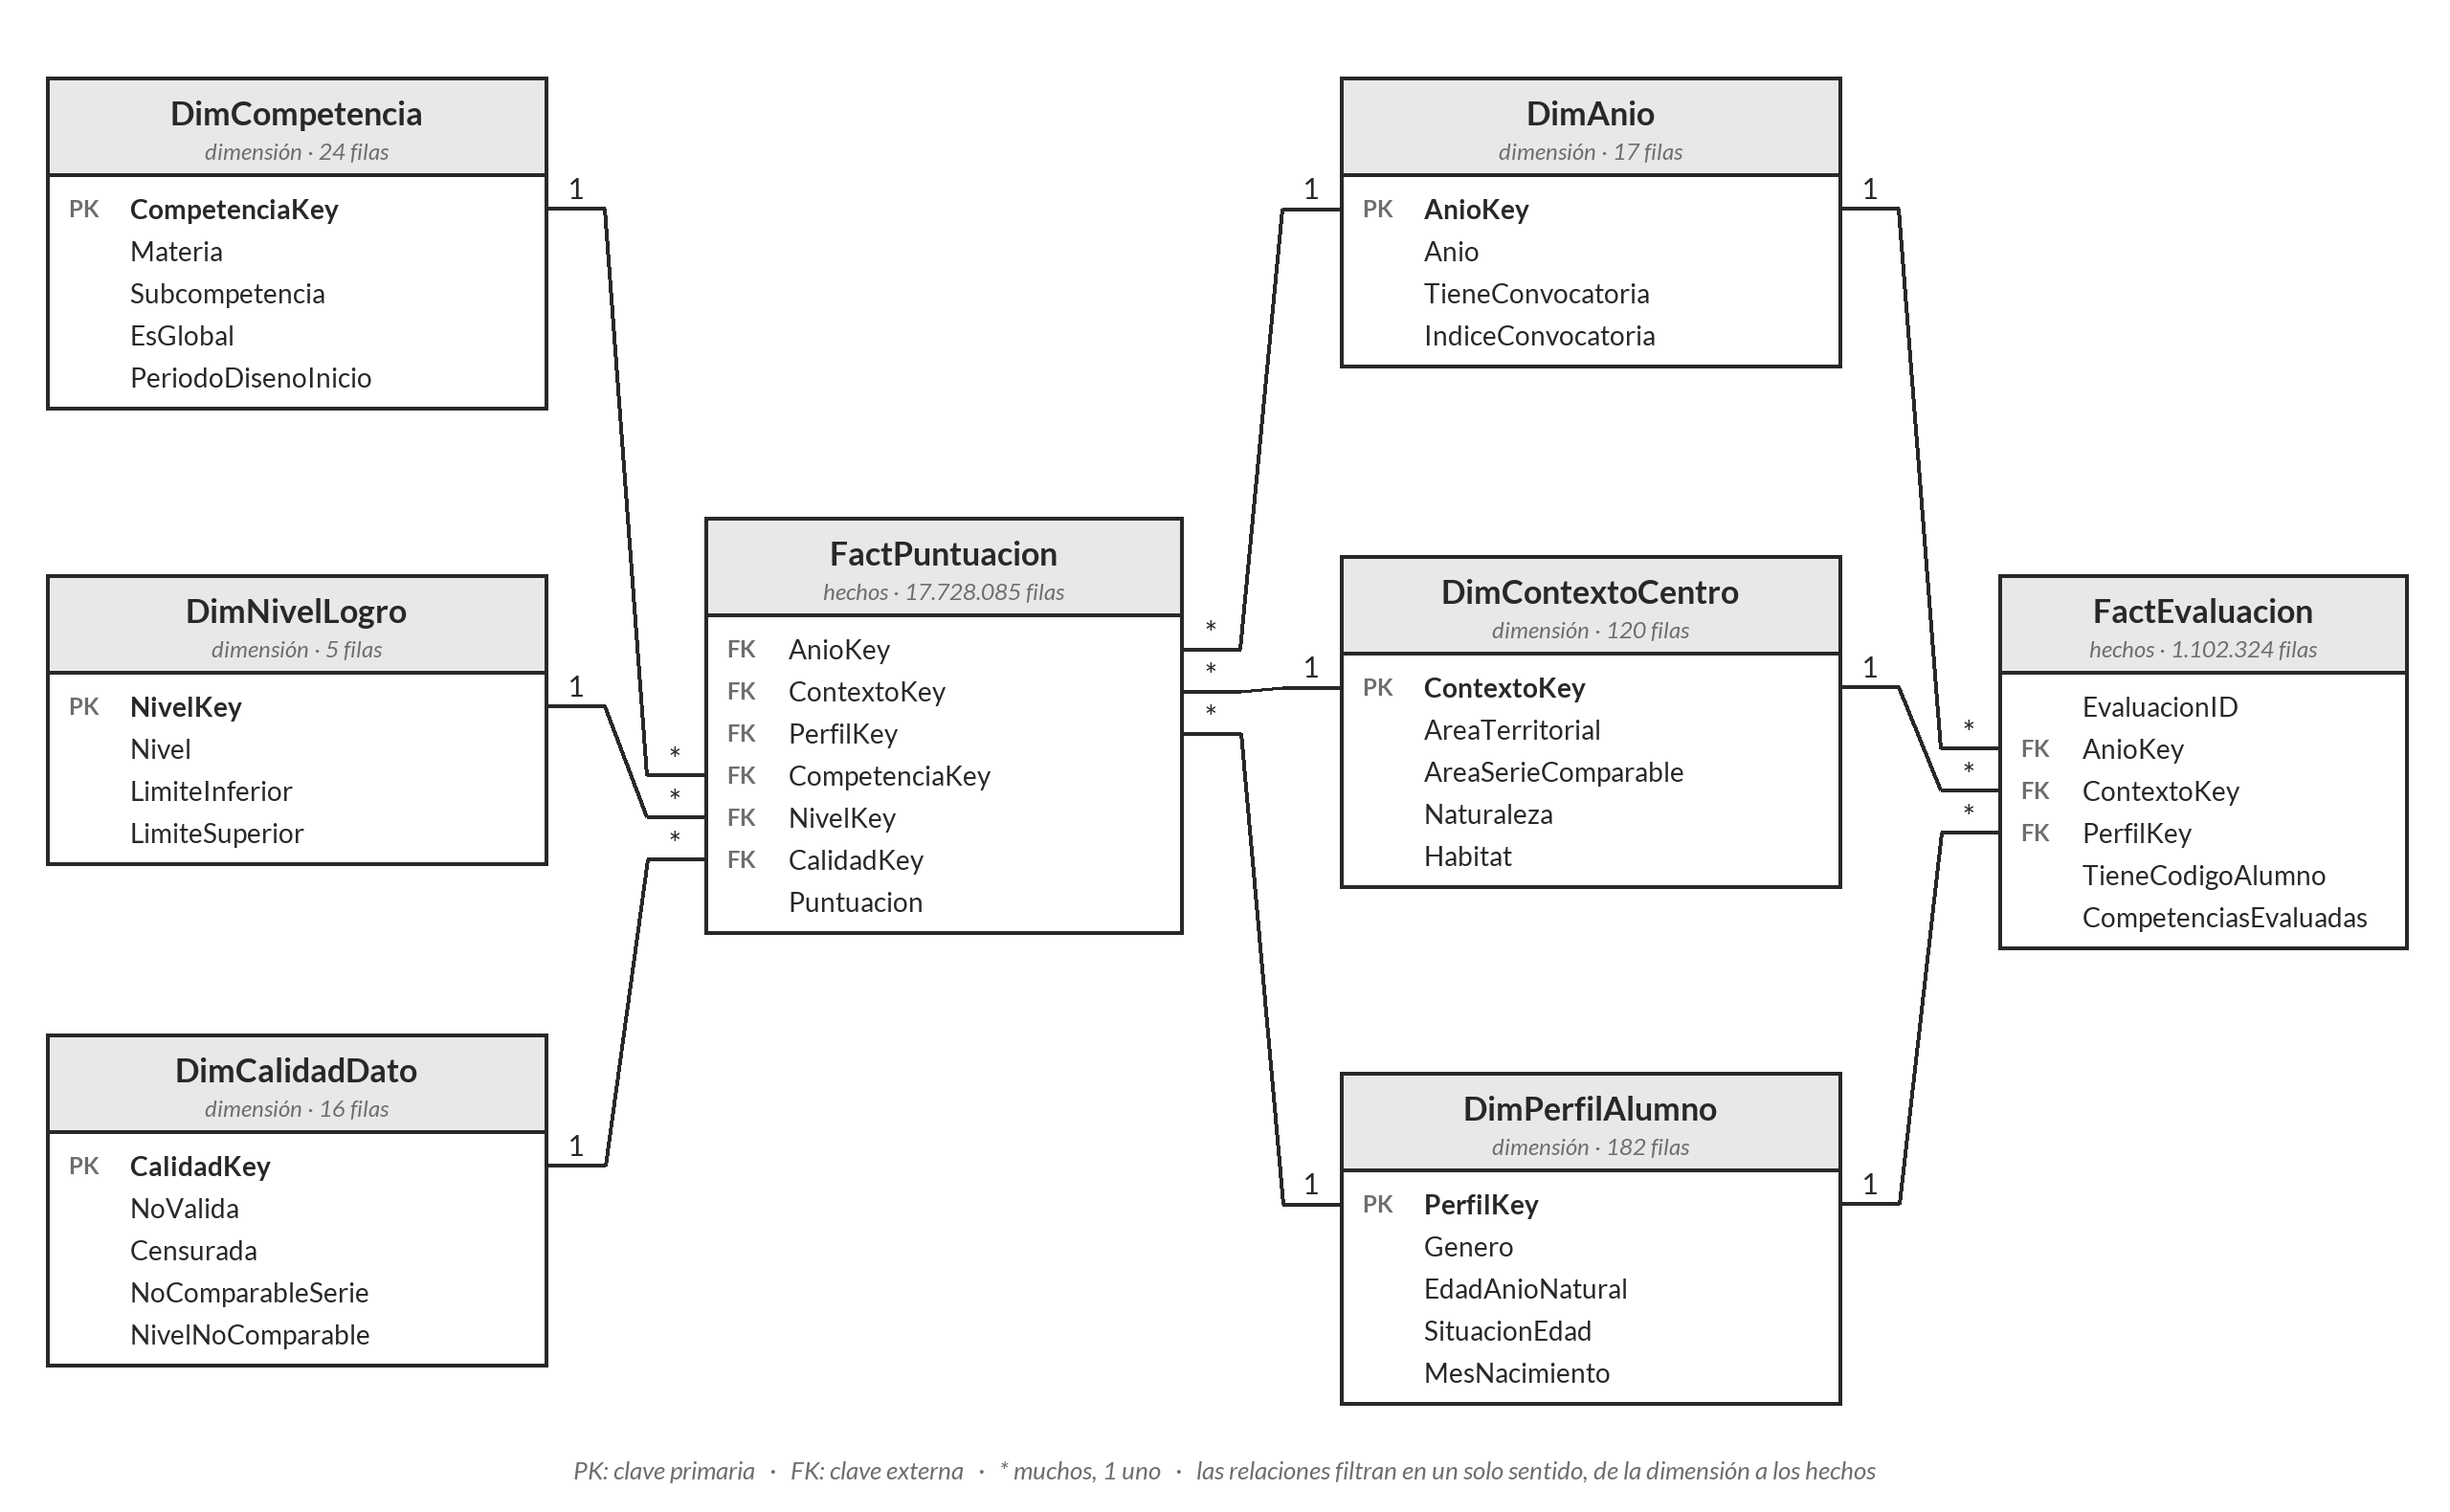
\includegraphics[width=\textwidth]{imagenes/diseno/esquema_estrella.png}
\caption{Esquema en estrella del modelo dimensional (claves y columnas principales).}
\label{fig:esquema_estrella}
\end{figure}

La Tabla~\ref{tab:ri_diseno} indica cómo garantiza el diseño cada restricción de integridad de la Tabla~\ref{tab:restricciones}. Cada una se comprueba además con una prueba de la validación independiente, que se ejecuta sobre las tablas que produce la réplica de la ETL.

\begin{table}[H]
\centering
\small
\setstretch{1.0}\renewcommand{\arraystretch}{1.1}
\begin{tabularx}{\textwidth}{@{} p{1.1cm} X @{}}
\toprule
\textbf{ID} & \textbf{Cómo se garantiza en el modelo dimensional} \\ \midrule
RI1 & Cada dimensión tiene una clave determinista única, y ningún hecho apunta a una clave que no exista. El contexto se identifica por la combinación codificada de área, titularidad y hábitat. \\ \addlinespace
RI2 & \texttt{DimCompetencia} guarda el periodo de vigencia de cada elemento (\texttt{AnioInicio}, \texttt{AnioFin}). Ninguna puntuación queda fuera de ese periodo, y el año de inicio coincide con el primer año con datos de cada columna. \\ \addlinespace
RI3 & La ETL asigna el nivel 0 \guillemotleft{}No aplica\guillemotright{} a toda subcompetencia y un nivel de 1 a 4 a toda competencia, según su valor. \\ \addlinespace
RI4 & \texttt{DimNivelLogro} guarda los límites de cada nivel. La ETL incluye el límite inferior y excluye el superior: 54,99 queda en el nivel bajo y 55,00 en el medio-bajo. \\ \addlinespace
RI5 & \texttt{DimAnio} marca 2020 sin convocatoria y los hechos no tienen ninguna fila de ese año. \\ \addlinespace
RI6 & La ETL deja la edad en blanco si queda fuera de 10 a 14 años. \\ \addlinespace
RI7 & La carga se detiene si una puntuación no está entre 0 y 100 (Sección~\ref{sec:reglas_limpieza}). \\ \bottomrule
\end{tabularx}
\caption{Restricciones de integridad en el modelo dimensional.}
\label{tab:ri_diseno}
\end{table}

\subsection{Tablas de hechos}
\label{sec:tablas_hechos}
El modelo tiene dos tablas de hechos, una por cada proceso que se mide: la participación del alumnado en la prueba y el resultado obtenido en cada competencia. La Tabla~\ref{tab:hechos} indica la granularidad de cada una, es decir, qué representa una fila.

\begin{table}[H]
\centering
\small
\setstretch{1.0}\renewcommand{\arraystretch}{1.1}
\begin{tabularx}{\textwidth}{@{} >{\raggedright\arraybackslash}p{2.7cm} X >{\raggedright\arraybackslash}p{2.0cm} >{\raggedright\arraybackslash}p{4.6cm} @{}}
\toprule
\textbf{Tabla} & \textbf{Granularidad} & \textbf{Filas} & \textbf{Columnas} \\ \midrule
\texttt{FactEvaluacion} & Un registro del fichero: un alumno evaluado en una convocatoria. & 1.102.324 & \texttt{EvaluacionID}, \texttt{AnioKey}, \texttt{ContextoKey}, \texttt{PerfilKey}, \texttt{TieneCodigoAlumno}, \texttt{CompetenciasEvaluadas}. \\ \addlinespace
\texttt{FactPuntuacion} & Una puntuación no nula de un registro en una de las 24 columnas de puntuación. & 17.728.085 (4.769.851 de competencias) & \texttt{AnioKey}, \texttt{ContextoKey}, \texttt{PerfilKey}, \texttt{CompetenciaKey}, \texttt{NivelKey}, \texttt{CalidadKey}, \texttt{Puntuacion}. \\ \bottomrule
\end{tabularx}
\caption{Granularidad de las tablas de hechos.}
\label{tab:hechos}
\end{table}

\texttt{FactPuntuacion} se obtiene despivotando las 24 columnas de puntuación del fichero: cada columna pasa a ser una fila con la clave de su elemento evaluado. Así la competencia es una dimensión más y una sola medida sirve para las 24 columnas, en lugar de repetir cada KPI por columna. Según la convocatoria, la tabla tiene de 589.644 filas (2009) a 1.466.352 (2019), porque el número de subcompetencias evaluadas cambia de un año a otro. No guarda el identificador de la evaluación, que ninguna medida necesita y que añadiría 17,7 millones de valores distintos al modelo.

\texttt{FactEvaluacion} existe para contar el alumnado. Si se contara a partir de las puntuaciones, el resultado dependería de la competencia filtrada y de cuántas subcompetencias tiene cada una. Como \texttt{FactEvaluacion} no se relaciona con \texttt{DimCompetencia}, el número de alumnos evaluados es el mismo sea cual sea la competencia elegida. \texttt{CompetenciasEvaluadas} cuenta las competencias con puntuación de cada alumno, y \texttt{TieneCodigoAlumno} indica si el registro original tenía código, sin guardarlo (RNF08).

\subsection{Dimensiones}
\label{sec:dimensiones}
Las seis dimensiones dan el contexto en el que se analizan los hechos. Cinco son estáticas: la ETL las genera a partir de tablas de códigos escritas en Power Query y no leen el fichero. La sexta, \texttt{DimAnio}, se deriva de los años presentes en el fichero, para que una convocatoria nueva aparezca sin cambiar nada (RNF09).

\texttt{DimAnio} tiene una fila por año de 2009 a 2025. \texttt{IndiceConvocatoria} numera de 1 a 16 solo los años con prueba y es la base de todas las comparaciones temporales: la convocatoria anterior a 2021 es 2019, no 2020. \texttt{NotaConvocatoria} guarda los avisos de 2020 (sin prueba por la COVID-19) y de 2021 (se compara con 2019).

\texttt{DimContextoCentro} tiene 120 filas, todas las combinaciones de 15 códigos de área territorial (uno de ellos para el área desconocida), 2 titularidades y 4 hábitats, aunque en los datos solo aparecen 85. Generar todas las combinaciones garantiza que cualquier registro encuentre su contexto sin consultar el fichero. La reorganización territorial de 2024 cambió el perímetro de varias áreas, así que la dimensión tiene una columna \texttt{AreaSerieComparable} que las agrupa en series con el mismo perímetro a lo largo del tiempo, y otra, \texttt{AreaConRupturaSerie}, que marca las afectadas. El fichero llama al área \guillemotleft{}Barcelona Comarques\guillemotright{} en 2024 y \guillemotleft{}Barcelonès\guillemotright{} en 2025, con el mismo perímetro y casi el mismo alumnado (5.386 y 5.408 alumnos), y el informe oficial de 2024 ya la publica como \guillemotleft{}Barcelonès\guillemotright{}. Por eso el modelo la muestra como \guillemotleft{}Barcelonès\guillemotright{} desde 2024 y reserva \guillemotleft{}Barcelona Comarques\guillemotright{} para el área anterior, hasta 2023, que tenía otro perímetro (RNF04). Girona pierde en 2024 la parte de la Cerdanya que pasa a Alt Pirineu i Aran, alrededor del 1\,\% de su alumnado. Se mantiene como serie propia porque el efecto sobre su media es de una o dos décimas como máximo, menos que el umbral del estado del KPI.

\texttt{DimPerfilAlumno} tiene 182 filas: 2 géneros, 7 combinaciones válidas de edad y situación de edad y 13 valores del mes de nacimiento (los 12 meses y \guillemotleft{}No informado\guillemotright{}). La edad es la del año natural, porque el fichero no trae la fecha de la prueba. En 2010 la edad y el hábitat no son fiables y se marcan así, sin imputarlos.

\texttt{DimCompetencia} tiene 24 filas, una por columna de puntuación: 6 competencias y 18 subcompetencias. Además del periodo de vigencia, guarda el inicio del periodo de diseño estable de la prueba (\texttt{PeriodoDisenoInicio}), que limita las comparaciones temporales (Sección~\ref{sec:fichas_kpis}), y marca el francés como competencia informativa, porque lo hace una muestra muy pequeña (entre 243 y 505 alumnos al año).

\texttt{DimNivelLogro} tiene los cuatro niveles internos del TFG (bajo, medio-bajo, medio-alto y alto, con cortes en 55, 70 y 85) y el miembro \guillemotleft{}No aplica\guillemotright{}. Los cortes se justifican en la Sección~\ref{sec:semaforos}.

\texttt{DimCalidadDato} tiene las 16 combinaciones de las cuatro marcas de calidad que asigna la ETL (RF04): no válida (bit 1), censurada (bit 2), escala no comparable en la serie (bit 4) y nivel no comparable (bit 8). Cada puntuación lleva una sola clave en lugar de cuatro columnas de 17,7 millones de filas, y cada KPI decide qué marcas excluye. La Sección~\ref{sec:reglas_limpieza} indica qué celdas recibe cada marca.

Las dimensiones tienen dos jerarquías. En \texttt{DimCompetencia}, cada competencia agrupa sus subcompetencias, y en \texttt{DimContextoCentro}, cada serie comparable agrupa sus áreas territoriales. Los atributos de texto se ordenan con una columna numérica oculta, de modo que las áreas, los niveles o las situaciones de edad aparecen en su orden lógico y no en el alfabético.

\subsection{Diccionario de datos}
\label{sec:diccionario_datos}
La Tabla~\ref{tab:diccionario} recoge las columnas visibles de las dimensiones, que son las que el usuario ve en los filtros y en los gráficos. Las claves, los códigos y las columnas de orden están ocultos, igual que todas las columnas de las tablas de hechos (Tabla~\ref{tab:hechos}), que solo se usan a través de las medidas. El diccionario completo, con todas las columnas, sus tipos y su origen, está en el documento del modelo del repositorio, y cada tabla y cada columna tiene además una descripción dentro del propio modelo de Power BI.

{\small\setstretch{1.0}\renewcommand{\arraystretch}{1.1}
\begin{longtable}{@{} >{\raggedright\arraybackslash}p{4.2cm} >{\raggedright\arraybackslash}p{1.6cm} p{8.5cm} @{}}
\toprule
\textbf{Columna} & \textbf{Tipo} & \textbf{Descripción} \\ \midrule
\endfirsthead
\toprule
\textbf{Columna} & \textbf{Tipo} & \textbf{Descripción} \\ \midrule
\endhead
\bottomrule
\caption{Diccionario de datos: columnas visibles de las dimensiones.}\label{tab:diccionario}
\endlastfoot
\multicolumn{3}{@{}l}{\textit{DimAnio}} \\
\texttt{Anio} & Entero & Año de la convocatoria (2009--2025). \\
\texttt{Curso} & Texto & Curso escolar, por ejemplo \guillemotleft{}2024-2025\guillemotright{}. \\
\texttt{TieneConvocatoria} & Booleano & Falso en 2020, año sin prueba. \\
\texttt{EsUltimaConvocatoria} & Booleano & Verdadero en la última convocatoria cargada. \\
\texttt{NotaConvocatoria} & Texto & Aviso de 2020 y de 2021; vacío en el resto. \\ \addlinespace
\multicolumn{3}{@{}l}{\textit{DimContextoCentro}} \\
\texttt{AreaTerritorial} & Texto & Área territorial (15 valores, con \guillemotleft{}Desconocida\guillemotright{}). \\
\texttt{AreaPerimetro2025} & Texto & Área a la que corresponde el territorio con la organización de 2025. \\
\texttt{AreaSerieComparable} & Texto & Serie de perímetro constante a la que pertenece el área. \\
\texttt{AreaConRupturaSerie} & Booleano & Verdadero en las áreas afectadas por la reorganización de 2024. \\
\texttt{RupturaHabitat2024} & Booleano & Verdadero en Girona y en Maresme - Vallès Oriental, que cambian la clasificación del hábitat en 2024. \\
\texttt{Naturaleza} & Texto & Titularidad del centro: Pública o Privada (incluye la concertada). En la interfaz se rotula \guillemotleft{}Titularidad\guillemotright{}. \\
\texttt{Habitat} & Texto & Tamaño del municipio: hasta 10.000, de 10.001 a 100.000 o más de 100.000 habitantes, o \guillemotleft{}No fiable\guillemotright{}. \\ \addlinespace
\multicolumn{3}{@{}l}{\textit{DimPerfilAlumno}} \\
\texttt{Genero} & Texto & Niña o Niño. \\
\texttt{EdadAnioNatural} & Entero & Edad en el año de la convocatoria (10--14) o en blanco. \\
\texttt{SituacionEdad} & Texto & Adelantado, edad teórica (12 años), retraso de 1 o de 2 años, no fiable (2010) o desconocida. \\
\texttt{MesNacimiento} & Entero & Mes de nacimiento (1--12) o en blanco. \\
\texttt{TrimestreNacimiento} & Texto & T1 a T4 o \guillemotleft{}No informado\guillemotright{}. \\ \addlinespace
\multicolumn{3}{@{}l}{\textit{DimCompetencia}} \\
\texttt{CampoOrigen} & Texto & Columna del fichero de la que procede la puntuación. \\
\texttt{CodigoMateria} & Texto & Columna de la puntuación global de la competencia. \\
\texttt{Materia} & Texto & Competencia (lengua catalana, lengua castellana, matemáticas, lengua inglesa, lengua francesa o ciencias). En la interfaz se rotula \guillemotleft{}Competencia\guillemotright{}. \\
\texttt{Subcompetencia} & Texto & Nombre de la subcompetencia o \guillemotleft{}Global\guillemotright{}. \\
\texttt{EsGlobal} & Booleano & Verdadero en las 6 competencias. \\
\texttt{AnioInicio}, \texttt{AnioFin} & Entero & Periodo de vigencia de la columna (RI2). \\
\texttt{PeriodoDisenoInicio} & Entero & Primer año con el diseño de prueba actual: 2017 o 2018. \\
\texttt{EsInformativa} & Booleano & Verdadero en lengua francesa. \\ \addlinespace
\multicolumn{3}{@{}l}{\textit{DimNivelLogro}} \\
\texttt{Nivel} & Texto & No aplica (subcompetencia), Bajo, Medio-bajo, Medio-alto o Alto. \\
\texttt{LimiteInferior}, \texttt{LimiteSuperior} & Decimal & Límites del nivel: 0, 55, 70, 85 y 100. \\ \addlinespace
\multicolumn{3}{@{}l}{\textit{DimCalidadDato}} \\
\texttt{NoValida}, \texttt{Censurada}, \texttt{NoComparableSerie}, \texttt{NivelNoComparable} & Booleano & Marcas de calidad de la puntuación (Sección~\ref{sec:reglas_limpieza}). \\
\texttt{DescripcionCalidad} & Texto & \guillemotleft{}Válido\guillemotright{} o la lista de problemas de la puntuación. \\
\end{longtable}}

Las columnas \texttt{Materia} y \texttt{Naturaleza} conservan su nombre técnico en el modelo, pero la interfaz las rotula \guillemotleft{}Competencia\guillemotright{} y \guillemotleft{}Titularidad\guillemotright{}, que son los términos de los informes oficiales (RNF04). Cambiar el nombre de las columnas obligaría a modificar la ETL, las medidas y la validación sin ninguna ventaja para el usuario.

El modelo se implementa en Power BI con estas decisiones físicas:
\begin{itemize}
    \item Modo de importación: los datos se cargan en el motor en memoria de Power BI y las consultas de los paneles no vuelven a leer el fichero.
    \item Claves enteras sin resumen automático, y \texttt{Puntuacion} como decimal fijo, que evita los errores de redondeo binario al sumar 17,7 millones de valores.
    \item Las medidas implícitas están desactivadas: el usuario solo puede usar las medidas definidas, que aplican las reglas de la Sección~\ref{sec:diseno_dax}.
    \item Cultura es-ES en el modelo y en la lectura del fichero, que usa la coma como separador decimal.
    \item Cada atributo de texto con orden propio se ordena por una columna oculta con un único valor por texto.
\end{itemize}

\section{Diseño de la ETL}
\label{sec:diseno_etl}
La ETL lee el fichero publicado, lo comprueba, lo limpia y carga las tablas del modelo dimensional (RF01--RF05). Se escribe en Power Query, el lenguaje de transformación de Power BI, y aplica las reglas de limpieza que salieron de la auditoría de los datos (tarea T7), documentadas en el informe de calidad con los identificadores R01 a R34.

\subsection{Flujo de consultas}
\label{sec:flujo_consultas}
La ETL se organiza en consultas que se ejecutan en este orden:
\begin{enumerate}
    \item \texttt{RutaDatos}: parámetro con la ruta del fichero CSV. Es lo único que se cambia para cargar el fichero en otro equipo.
    \item \texttt{stg\_Evaluaciones}: tabla intermedia (\textit{staging}) que no se carga en el modelo. Lee el fichero, comprueba su estructura y sus valores, unifica los códigos, corrige las columnas rotadas y calcula las claves de las dimensiones. Contiene casi todas las reglas de limpieza.
    \item Dimensiones: \texttt{DimAnio} se deriva de los años de \texttt{stg\_Evaluaciones}; las otras cinco son tablas de códigos escritas en la propia consulta.
    \item Hechos: \texttt{FactEvaluacion} toma las columnas de la evaluación. \texttt{FactPuntuacion} despivota las 24 columnas de puntuación y asigna a cada puntuación su competencia, su nivel de logro y su clave de calidad.
    \item \texttt{\_Medidas}: tabla vacía que solo agrupa las medidas DAX (Sección~\ref{sec:diseno_dax}).
\end{enumerate}

Ninguna consulta combina tablas (\textit{merge}): como las claves se calculan con fórmulas (Sección~\ref{sec:diseno_logico}), cada tabla de hechos tiene sus claves sin buscarlas en las dimensiones. Las tres consultas que dependen de \texttt{stg\_Evaluaciones} vuelven a leer el fichero, de modo que una actualización lo lee tres veces. Es el coste de no guardar una copia intermedia, y permite actualizar el modelo solo con sustituir el fichero (RNF09). La guía de uso del repositorio explica cómo cambiar la ruta y qué hacer en la primera actualización.

\subsection{Reglas de limpieza}
\label{sec:reglas_limpieza}
La Tabla~\ref{tab:reglas_etl} resume las reglas de limpieza en el orden en que las aplica la ETL. La última columna indica si la regla puede detener la carga. El informe de calidad describe cada regla, las filas a las que afecta y la evidencia que la justifica.

{\small\setstretch{1.0}\renewcommand{\arraystretch}{1.1}
\begin{longtable}{@{} p{10.2cm} >{\raggedright\arraybackslash}p{2.1cm} >{\raggedright\arraybackslash}p{2.0cm} @{}}
\toprule
\textbf{Paso} & \textbf{Regla} & \textbf{Detiene la carga} \\ \midrule
\endfirsthead
\toprule
\textbf{Paso} & \textbf{Regla} & \textbf{Detiene la carga} \\ \midrule
\endhead
\bottomrule
\caption{Reglas de limpieza que aplica la ETL, en orden.}\label{tab:reglas_etl}
\endlastfoot
\multicolumn{3}{@{}l}{\textit{Tabla intermedia (\texttt{stg\_Evaluaciones})}} \\
Lectura del fichero como texto y comprobación de que la cabecera tiene exactamente las 32 columnas esperadas. & R34 (en parte) & Sí \\ \addlinespace
Identificador de la evaluación: posición del registro en el fichero, antes de cualquier filtro. & R01 & No \\ \addlinespace
Eliminación de espacios y conversión de las cadenas vacías en valores nulos. & R05 & No \\ \addlinespace
Conversión de las 24 puntuaciones con la coma decimal; un valor no numérico o fuera de 0 a 100 es un error. & R02 & Sí \\ \addlinespace
Corrección de las columnas rotadas: lengua castellana en 2017 y lengua francesa en 2016. & R03, R04 & No \\ \addlinespace
Unificación de los códigos de género, titularidad y hábitat, que cambian entre convocatorias (por ejemplo, \textit{Públic} y \textit{Pública}); un código no previsto es un error. & R09--R11 & Sí \\ \addlinespace
Código del área territorial; el área vacía pasa a \guillemotleft{}Desconocida\guillemotright{} y un nombre no previsto es un error. & R13, R14 & Sí \\ \addlinespace
Hábitat \guillemotleft{}No fiable\guillemotright{} en 2010 y en 29 registros de Baix Llobregat de 2014. & R12 & No \\ \addlinespace
Edad en el año natural, mes de nacimiento y situación de edad; la edad queda en blanco si falta, si la fecha es dudosa o si está fuera de 10 a 14 años. & R16--R19, R21 & No \\ \addlinespace
Claves de año, contexto y perfil; el código de alumno se descarta y solo se guarda si existía. & R06 & No \\ \addlinespace
\multicolumn{3}{@{}l}{\textit{Tabla de hechos \texttt{FactPuntuacion}}} \\
Despivotado de las 24 columnas de puntuación, sin los valores nulos. & R33 & No \\ \addlinespace
Nivel de logro: 1 a 4 en las competencias según los cortes 55, 70 y 85; 0 en las subcompetencias. & R29 & No \\ \addlinespace
Marcas de calidad: no válida (expresión escrita de inglés 2015), censurada (puntuaciones acumuladas en un suelo artificial: expresión escrita de catalán 2018, y global y dos subcompetencias de inglés 2015), escala no comparable en la serie y nivel no comparable (inglés 2015 y 2016, matemáticas 2015 y 2019, catalán 2018 y francés 2022). & R25--R28 & No \\
\end{longtable}}

Las comprobaciones que detienen la carga generan un error con el nombre de la regla, el valor y el identificador del registro. Power BI, por defecto, carga una celda con error como vacía y solo muestra un aviso, así que la ETL busca los registros con error y, si encuentra alguno, hace fallar la consulta entera. La actualización se detiene, el modelo conserva los datos de la carga anterior y Power BI muestra el mensaje de la regla incumplida (RF05, CU01). Con el fichero actual no se dispara ninguna: no hay valores fuera de rango ni códigos no previstos.

El informe de calidad proponía mandar los códigos no previstos a una categoría \guillemotleft{}Desconocido\guillemotright{} y fijar el número de registros del fichero. La ETL detiene la carga en el primer caso, porque un código nuevo no debe pasar inadvertido (RF05), y no fija el número de registros, porque eso impediría cargar una convocatoria nueva (RNF09). El recuento de registros por convocatoria y la corrección de las columnas rotadas se comprueban en la validación independiente, no en la carga.

La puntuación global de cada competencia se carga tal como se publica y no se recalcula. En ciencias, los pesos publicados (42, 25 y 33\,\%) no reproducen la global del fichero, que es la media simple de las tres subcompetencias en el 100\,\% de los registros. Las medias oficiales también salen de la global publicada, así que recalcularla rompería la conciliación con ellas (RNF06).

Las reglas que solo añaden marcas informativas por registro quedan fuera del alcance mínimo y se documentan como extensiones en el documento del modelo del repositorio. Son, por ejemplo, la marca de código de alumno repetido en un mismo año (R07), la de repetición probable de curso (R08) y la de global incoherente con sus subcompetencias (R23).

\section{Diseño de la lógica analítica}
\label{sec:diseno_dax}
La lógica analítica calcula los KPIs del catálogo (Tabla~\ref{tab:kpis}) con medidas DAX, el lenguaje de cálculo de Power BI \cite{ferrari2019definitive}. Una medida no guarda ningún valor: se evalúa cada vez que cambia un filtro, con el contexto que define la selección del usuario (RF11). El modelo tiene 20 medidas en una tabla sin datos, \texttt{\_Medidas}, repartidas en carpetas: una con las medidas base (alumnos evaluados, número de puntuaciones y medias), una por cada perspectiva del CMI y una con el estado de los KPIs.

Todas las medidas siguen las mismas reglas:
\begin{itemize}
    \item Los KPIs de competencia solo usan las puntuaciones globales (\texttt{EsGlobal} verdadero). El filtro se añade al del usuario sin sustituirlo.
    \item \guillemotleft{}Cataluña\guillemotright{} es el mismo cálculo sin ningún filtro de \texttt{DimContextoCentro}, conservando los de año, competencia y perfil.
    \item Un KPI queda en blanco si se calcula sobre menos de 30 puntuaciones (RF14). La regla se aplica en las medidas de base y las demás la heredan (Sección~\ref{sec:semaforos}).
    \item Las comparaciones temporales navegan por \texttt{IndiceConvocatoria} y no restan un año, así que 2021 se compara con 2019. Solo usan las competencias cuyo diseño de prueba no ha cambiado desde la convocatoria de referencia.
\end{itemize}

\subsection{Fichas de los KPIs}
\label{sec:fichas_kpis}
La Tabla~\ref{tab:fichas_kpis} es la ficha resumida de cada KPI, agrupada por perspectiva. Indica cómo se calcula, qué filtros respeta o sustituye, qué puntuaciones excluye y en qué panel aparece. Las fichas completas, con el sentido favorable, los casos en blanco y la fórmula DAX de cada medida, están en el documento de fichas de los KPIs del repositorio.

{\small\setstretch{1.0}\renewcommand{\arraystretch}{1.1}
\begin{longtable}{@{} >{\raggedright\arraybackslash}p{2.6cm} p{5.9cm} p{4.3cm} >{\raggedright\arraybackslash}p{1.1cm} @{}}
\toprule
\textbf{KPI} & \textbf{Cálculo} & \textbf{Filtros y exclusiones} & \textbf{Panel} \\ \midrule
\endfirsthead
\toprule
\textbf{KPI} & \textbf{Cálculo} & \textbf{Filtros y exclusiones} & \textbf{Panel} \\ \midrule
\endhead
\bottomrule
\caption{Fichas resumidas de los KPIs.}\label{tab:fichas_kpis}
\endlastfoot
\multicolumn{4}{@{}l}{\textit{Rendimiento académico}} \\
K01 Puntuación media & Media de las puntuaciones globales. Sin filtro de competencia, promedia todas las competencias. & Respeta todos los filtros. & E, T, O \\ \addlinespace
K02 Puntuación por subcompetencia & Media de las puntuaciones de las subcompetencias. & Excluye las no válidas. Para series temporales hay que filtrar las escalas no comparables. & O \\ \addlinespace
K03 \% de alumnado en nivel bajo & Porcentaje de puntuaciones globales por debajo de 55. Con una competencia seleccionada equivale al porcentaje de alumnado. & Excluye las censuradas y las de nivel no comparable. Ignora el filtro de nivel. & E \\ \addlinespace
\multicolumn{4}{@{}l}{\textit{Equidad e inclusión}} \\
K04 Brecha de género & K01 de los niños menos K01 de las niñas. Positivo: los niños puntúan más. & Sustituye el filtro de género. & T \\ \addlinespace
K05 Brecha pública--privada & K01 de los centros públicos menos K01 de los privados, concertados incluidos. & Sustituye el filtro de titularidad. & T \\ \addlinespace
K06 Dispersión & Desviación típica poblacional de las puntuaciones globales. & Excluye las censuradas. & E \\ \addlinespace
\multicolumn{4}{@{}l}{\textit{Territorio y entorno}} \\
K07 Desviación respecto a Cataluña & K01 de la selección menos K01 de Cataluña. Sin área ni contexto seleccionados vale 0. & Respeta año, competencia y perfil. & T, O \\ \addlinespace
K08 Diferencia urbano--rural & K01 en municipios de más de 100.000 habitantes menos K01 en los de hasta 10.000. & Sustituye el filtro de hábitat. 2010 queda en blanco. & T \\ \addlinespace
K09 Posición del área & Posición del área por K01, de mayor a menor; los empates comparten posición. & Requiere una sola área. No cuenta el área desconocida ni el francés solo. & T \\ \addlinespace
\multicolumn{4}{@{}l}{\textit{Eficiencia y progreso}} \\
K10 Variación interanual & K01 de la convocatoria menos K01 de la anterior. & Requiere un solo año. Solo competencias con diseño estable. Desde 2018. & E \\ \addlinespace
K11 Tendencia de 5 convocatorias & Diferencia de K01 entre la convocatoria y la cuarta anterior, dividida entre 4. & Igual que K10. Desde 2022. & E \\ \addlinespace
K12 \% de competencias que mejoran & Porcentaje de competencias con K10 de 1 punto o más sobre las que tienen K10. & Sin el francés. Desde 2018. & E \\
\end{longtable}}

Las fórmulas de K01 y K10 muestran cómo se aplican las reglas comunes. K01 aplica el mínimo de 30 puntuaciones y el filtro de las globales. \texttt{KEEPFILTERS} añade la condición sin quitar la competencia que haya elegido el usuario.

\par\vspace{2ex}\noindent\begin{minipage}{\textwidth}\small\setstretch{1.0}
\begin{verbatim}
K01 Puntuación media competencia =
VAR _n = [Puntuaciones globales]
RETURN
    IF (
        _n >= 30,
        CALCULATE (
            AVERAGE ( FactPuntuacion[Puntuacion] ),
            KEEPFILTERS ( DimCompetencia[EsGlobal] = TRUE () )
        )
    )
\end{verbatim}
\end{minipage}\par\vspace{2.5ex}

K03 sigue el mismo esquema con dos condiciones más: excluye las puntuaciones censuradas y las de nivel no comparable, y quita el filtro de nivel de logro para que el porcentaje no cambie si el usuario filtra un nivel.

K10 busca la convocatoria anterior por su índice y compara las dos medias con las mismas competencias: las que tienen un diseño de prueba estable desde la convocatoria anterior.

\par\vspace{2ex}\noindent\begin{minipage}{\textwidth}\footnotesize\setstretch{1.0}
\begin{verbatim}
K10 Variación interanual =
VAR _i =
  CALCULATE (
    SELECTEDVALUE ( DimAnio[IndiceConvocatoria] ),
    KEEPFILTERS ( DimAnio[TieneConvocatoria] = TRUE () )
  )
RETURN
  IF (
    _i > 1,
    VAR _anioAnterior =
      CALCULATE (
        MAX ( DimAnio[Anio] ),
        REMOVEFILTERS ( DimAnio ),
        DimAnio[IndiceConvocatoria] = _i - 1
      )
    VAR _actual =
      CALCULATE (
        [K01 Puntuación media competencia],
        KEEPFILTERS ( DimCompetencia[PeriodoDisenoInicio] <= _anioAnterior )
      )
    VAR _anterior =
      CALCULATE (
        [K01 Puntuación media competencia],
        REMOVEFILTERS ( DimAnio ),
        DimAnio[IndiceConvocatoria] = _i - 1,
        KEEPFILTERS ( DimCompetencia[PeriodoDisenoInicio] <= _anioAnterior )
      )
    RETURN
      IF ( NOT ISBLANK ( _actual ) && NOT ISBLANK ( _anterior ),
           _actual - _anterior )
  )
\end{verbatim}
\end{minipage}\par\vspace{2.5ex}

Tres KPIs necesitan una aclaración sobre la calidad de los datos:
\begin{itemize}
    \item K03 y K06 excluyen las puntuaciones censuradas, que son las de una columna y un año con muchas puntuaciones acumuladas en un mismo valor mínimo. En inglés 2015, el 12,9\,\% de las globales vale exactamente 48,79; una desviación típica calculada sobre esa acumulación sería un artefacto. Catalán 2018 tiene la cola baja comprimida pero ninguna acumulación, así que se marca con nivel no comparable: K03 la excluye y K06 la incluye con una advertencia en la descripción de la medida.
    \item K10, K11 y K12 solo comparan competencias cuya prueba no ha cambiado de diseño. El periodo de diseño estable empieza en 2017 en matemáticas, inglés y francés, y en 2018 en catalán, castellano y ciencias. Por eso K10 y K12 tienen valor desde 2018 y K11 desde 2022.
    \item Las puntuaciones no están equiparadas entre convocatorias, porque las pruebas no comparten preguntas de anclaje. La diferencia entre dos años mezcla el cambio de rendimiento con el de dificultad de la prueba, así que K10, K11 y K12 son orientativos y los paneles lo advierten (RF15).
\end{itemize}

Los KPIs se han comprobado con la validación independiente en Python, que los calcula con otra implementación a partir del mismo fichero. Las 72 medias de Cataluña por competencia y convocatoria cumplen el criterio de aceptación de 0,5 puntos frente a las oficiales (RNF06), con una diferencia máxima de 0,30. La validación usa además un umbral de alerta de 0,2: 70 de las 72 medias quedan dentro, y las dos restantes (inglés 2016, +0,24; francés 2024, +0,30) están explicadas en el informe de calidad.

\subsection{Estado de los KPIs y referencias}
\label{sec:semaforos}
El estado de un KPI indica si su valor es favorable, neutro o desfavorable respecto a una referencia (RF13). Se calcula para tres KPIs, K01, K03 y K10, y cada uno se muestra en los paneles donde su referencia tiene sentido (Tabla~\ref{tab:semaforos}).

\begin{table}[H]
\centering
\small
\setstretch{1.0}\renewcommand{\arraystretch}{1.1}
\begin{tabularx}{\textwidth}{@{} >{\raggedright\arraybackslash}p{2.0cm} X >{\raggedright\arraybackslash}p{2.6cm} >{\raggedright\arraybackslash}p{3.2cm} @{}}
\toprule
\textbf{Estado} & \textbf{Referencia} & \textbf{Umbral} & \textbf{Panel} \\ \midrule
Estado K01 & Con un área o un contexto seleccionado, Cataluña (K07). Sin selección, la convocatoria anterior (K10). & $\pm 1$ punto con K07; $\pm 0{,}5$ puntos con K10 & Táctico y operativo \\ \addlinespace
Estado K03 & K03 de Cataluña. & $\pm 2$ puntos porcentuales & Táctico y operativo \\ \addlinespace
Estado K10 & Cero: la variación respecto a la convocatoria anterior. & $\pm 0{,}5$ puntos & Estratégico (tarjeta y tabla por competencia) \\ \bottomrule
\end{tabularx}
\caption{Estado de los KPIs: referencia, umbral y panel en que se muestra.}
\label{tab:semaforos}
\end{table}

En el panel estratégico no hay un territorio con el que comparar, porque muestra toda Cataluña. Allí el estado de K01 coincidiría con el de K10 y el de K03 valdría siempre neutro, ya que compararía Cataluña consigo misma, así que solo se muestra el de K10. Tampoco hay un estado temporal de K03: el porcentaje por debajo de un corte fijo depende mucho de la dificultad de cada prueba (en ciencias pasa del 13,2\,\% al 26,9\,\% de 2024 a 2025) y las pruebas no están equiparadas.

Cada estado es una medida que devuelve 1, 0 o $-1$. Una cadena de formato la muestra como \guillemotleft{}$\blacktriangle$ Favorable\guillemotright{}, \guillemotleft{}$\bullet$ Neutro\guillemotright{} o \guillemotleft{}$\blacktriangledown$ Desfavorable\guillemotright{}. El estado se lee por el símbolo y la palabra, sin depender del color (RNF05), y no hace falta formato condicional. Los umbrales son propuestas del TFG. Están en las medidas, así que se pueden ajustar sin cambiar el modelo.

Los niveles de logro usan cortes fijos en 55, 70 y 85 puntos, comunes a todas las competencias y convocatorias. Son niveles internos del TFG, porque el fichero no trae los niveles oficiales. Cada corte cae dentro de la horquilla oficial: nivel mínimo entre 50 y 60, nivel óptimo en 70 y nivel alto entre 80 y 90 \cite{csase_resultats}. Se han comparado con los porcentajes oficiales de 35 combinaciones de competencia y año (2018--2025). Con el corte en 55, el error medio en el nivel bajo es de 2,70 puntos porcentuales y el sesgo, de $-0{,}14$. Con un corte en 50 el sesgo sería de $-4{,}39$, y con uno en 60, de $+5{,}22$. Unos cortes distintos para cada año reproducirían mejor los porcentajes oficiales, pero dependerían de una tabla externa que habría que mantener a mano cada año (RNF09). Las convocatorias en las que el corte fijo no es fiable tienen la marca de nivel no comparable y no cuentan en K03.

La regla de las 30 puntuaciones (RF14) se aplica en K01, K02, K03, K06 y en la medida de la distribución por nivel de logro. Las demás medidas usan K01 y la heredan: una brecha o una variación queda en blanco si cualquiera de sus dos términos lo está. Por ejemplo, el francés del Vallès Occidental en 2025 queda en blanco porque tiene 24 puntuaciones, mientras que el de toda Cataluña ese año se muestra, con 243. En la distribución por nivel el mínimo se cuenta sobre el total de la competencia y no sobre cada nivel, de modo que un nivel con pocas puntuaciones no desaparece de una distribución válida. Esa medida aplica las mismas exclusiones que K03, así que el tramo bajo del gráfico coincide con K03.

\section{Diseño de la interfaz}
\label{sec:diseno_interfaz}
La interfaz es el informe de Power BI con los tres paneles, uno por perfil (RF16--RF18). Parte del prototipo de la Sección~\ref{sec:mockups} y lo concreta con los elementos visuales de Power BI y con las medidas de la Sección~\ref{sec:diseno_dax}. Primero se describe lo que comparten los tres paneles y después el diseño final de cada uno, con los cambios respecto al prototipo.

\subsection{Estructura común y navegación}
\label{sec:estructura_comun}
Los tres paneles mantienen la estructura del prototipo para que el usuario no tenga que aprender una disposición nueva en cada uno:
\begin{itemize}
    \item Arriba, una cabecera con el título del panel y, en la misma franja, los segmentadores desplegables.
    \item Debajo, una fila de tarjetas con los KPIs principales y su estado.
    \item En el centro, los gráficos y las tablas, que ocupan el resto del lienzo.
    \item Un aviso fijo sobre las limitaciones de los datos (RF15): las puntuaciones no están equiparadas, 2020 no tuvo prueba y 2021 se compara con 2019. En el panel estratégico va al pie, junto con la advertencia de que los niveles de logro son internos del TFG; en los otros dos, en el subtítulo de la cabecera.
\end{itemize}

Cada página tiene un lienzo de 1280 $\times$ 720 píxeles y todos los elementos quedan dentro: el borde derecho más alejado está en el píxel 1264 y el inferior en el 708 (RNF03). Para cambiar de panel se usan las pestañas de página de Power BI (CU10).

Los segmentadores de una misma columna están sincronizados entre los paneles: al cambiar de panel se conservan el año, la competencia, el área territorial, la titularidad, el hábitat y el género elegidos (RF10). El año es de selección única y se abre en la última convocatoria, 2025. Dentro de cada panel, seleccionar un elemento de un gráfico filtra o resalta los demás (CU05). Hay dos excepciones, configuradas en las interacciones del informe. El segmentador de año no filtra los gráficos de evolución, que muestran siempre todas las convocatorias (RF08). El segmentador de área no filtra las barras de desviación por área, que muestran siempre todas las áreas (RF09). En los gráficos de evolución el eje muestra también los años sin datos, de modo que 2020 aparece como un hueco y la línea no une 2019 con 2021.

Para la accesibilidad (RNF05), el estado de los KPIs se lee por el símbolo y la palabra (Sección~\ref{sec:semaforos}), y no solo por el color. Los cuatro niveles de logro usan una paleta divergente de naranja a violeta de ColorBrewer (PuOr) \cite{harrower2003colorbrewer}, que se distingue con deuteranopía y con protanopía. Cada elemento visual tiene un texto alternativo para los lectores de pantalla. El texto usa la fuente Segoe UI, con el título de la cabecera en 16 puntos y los subtítulos en gris, y la palabra \guillemotleft{}Aviso\guillemotright{} en rojo oscuro. Toda la interfaz está en castellano, con los términos de los informes oficiales (RNF04).

\subsection{Diseño final de los paneles}
\label{sec:paneles}
Las Figuras~\ref{fig:panel_estrategico} a \ref{fig:panel_operativo} muestran la disposición final de cada panel. Se generan con un script a partir de los ficheros del informe, de modo que cada caja tiene la posición, el tamaño, el título y los campos del elemento visual real. La guía de uso del repositorio explica cómo se usa cada panel.

\begin{figure}[H]
\centering
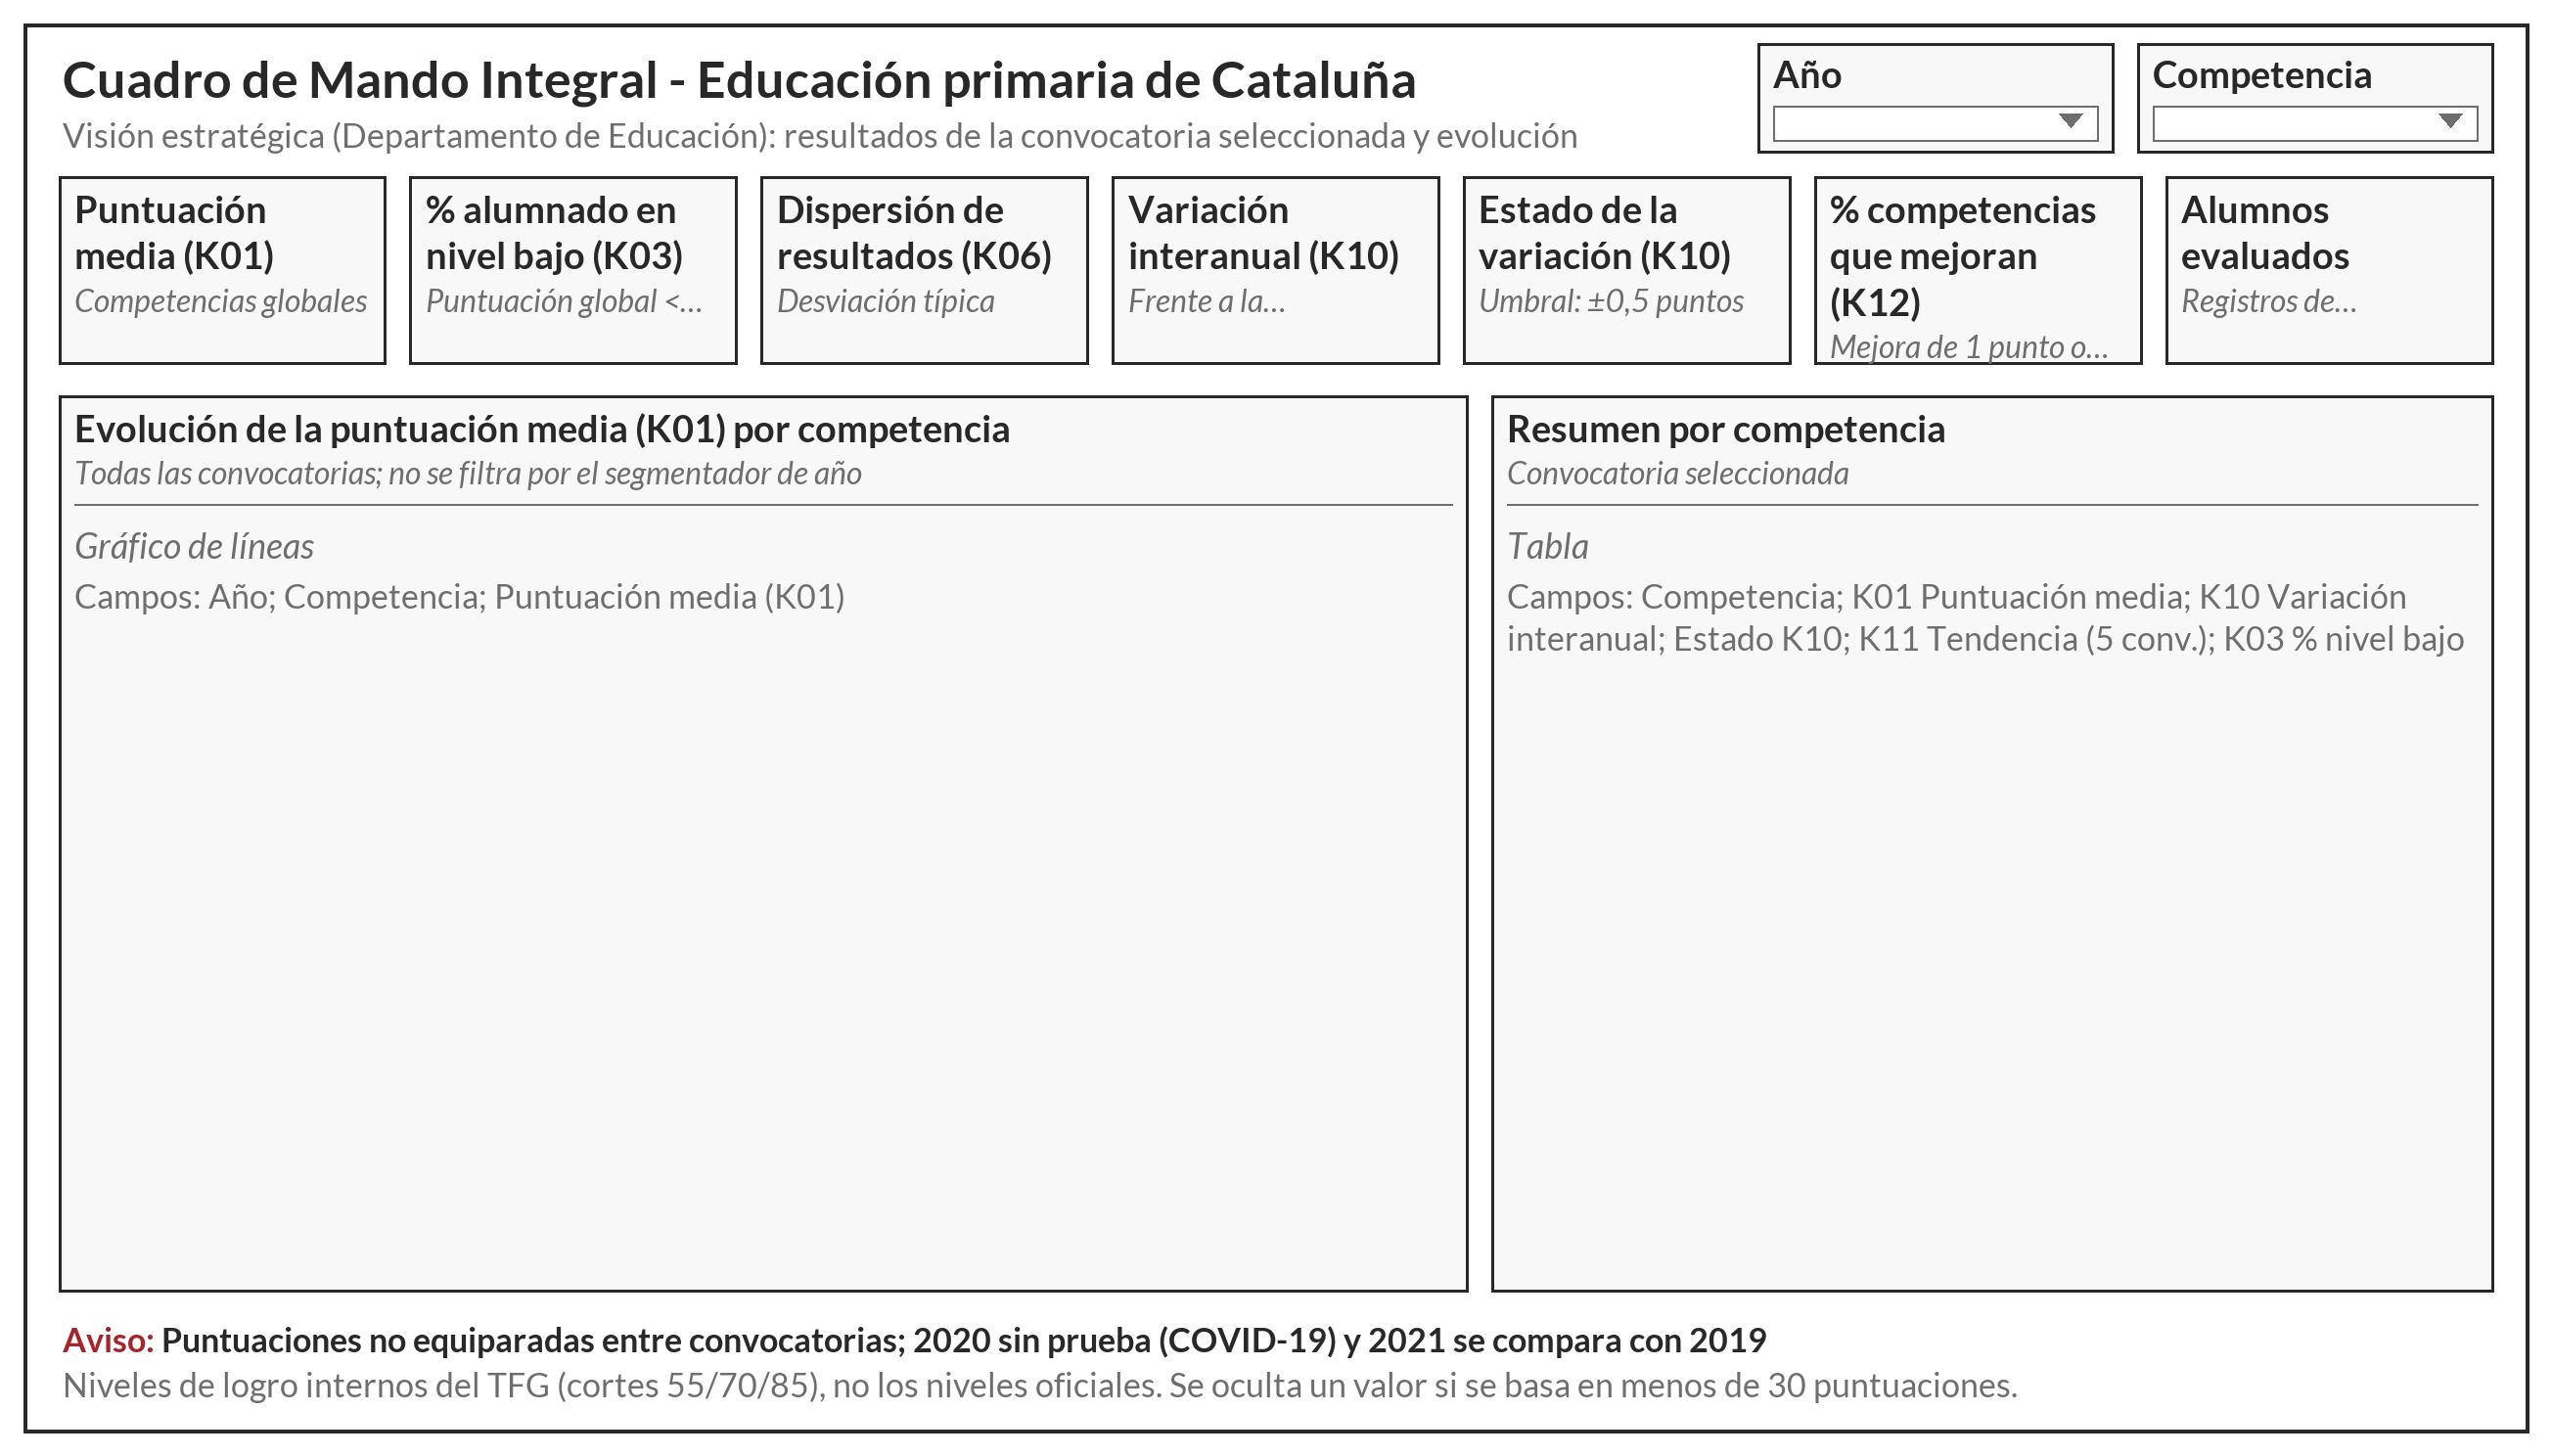
\includegraphics[width=\textwidth]{imagenes/diseno/panel_estrategico.png}
\caption{Disposición final del panel estratégico (Departamento de Educación).}
\label{fig:panel_estrategico}
\end{figure}

El panel estratégico (Figura~\ref{fig:panel_estrategico}) tiene los segmentadores de año y competencia y siete tarjetas: K01, K03, K06, K10 con su estado en una tarjeta propia, K12 y el alumnado evaluado. El gráfico de líneas muestra K01 de cada competencia en todas las convocatorias, y la tabla resume K01, K10 con su estado, K11 y K03 de cada competencia en la convocatoria elegida.

\begin{figure}[H]
\centering
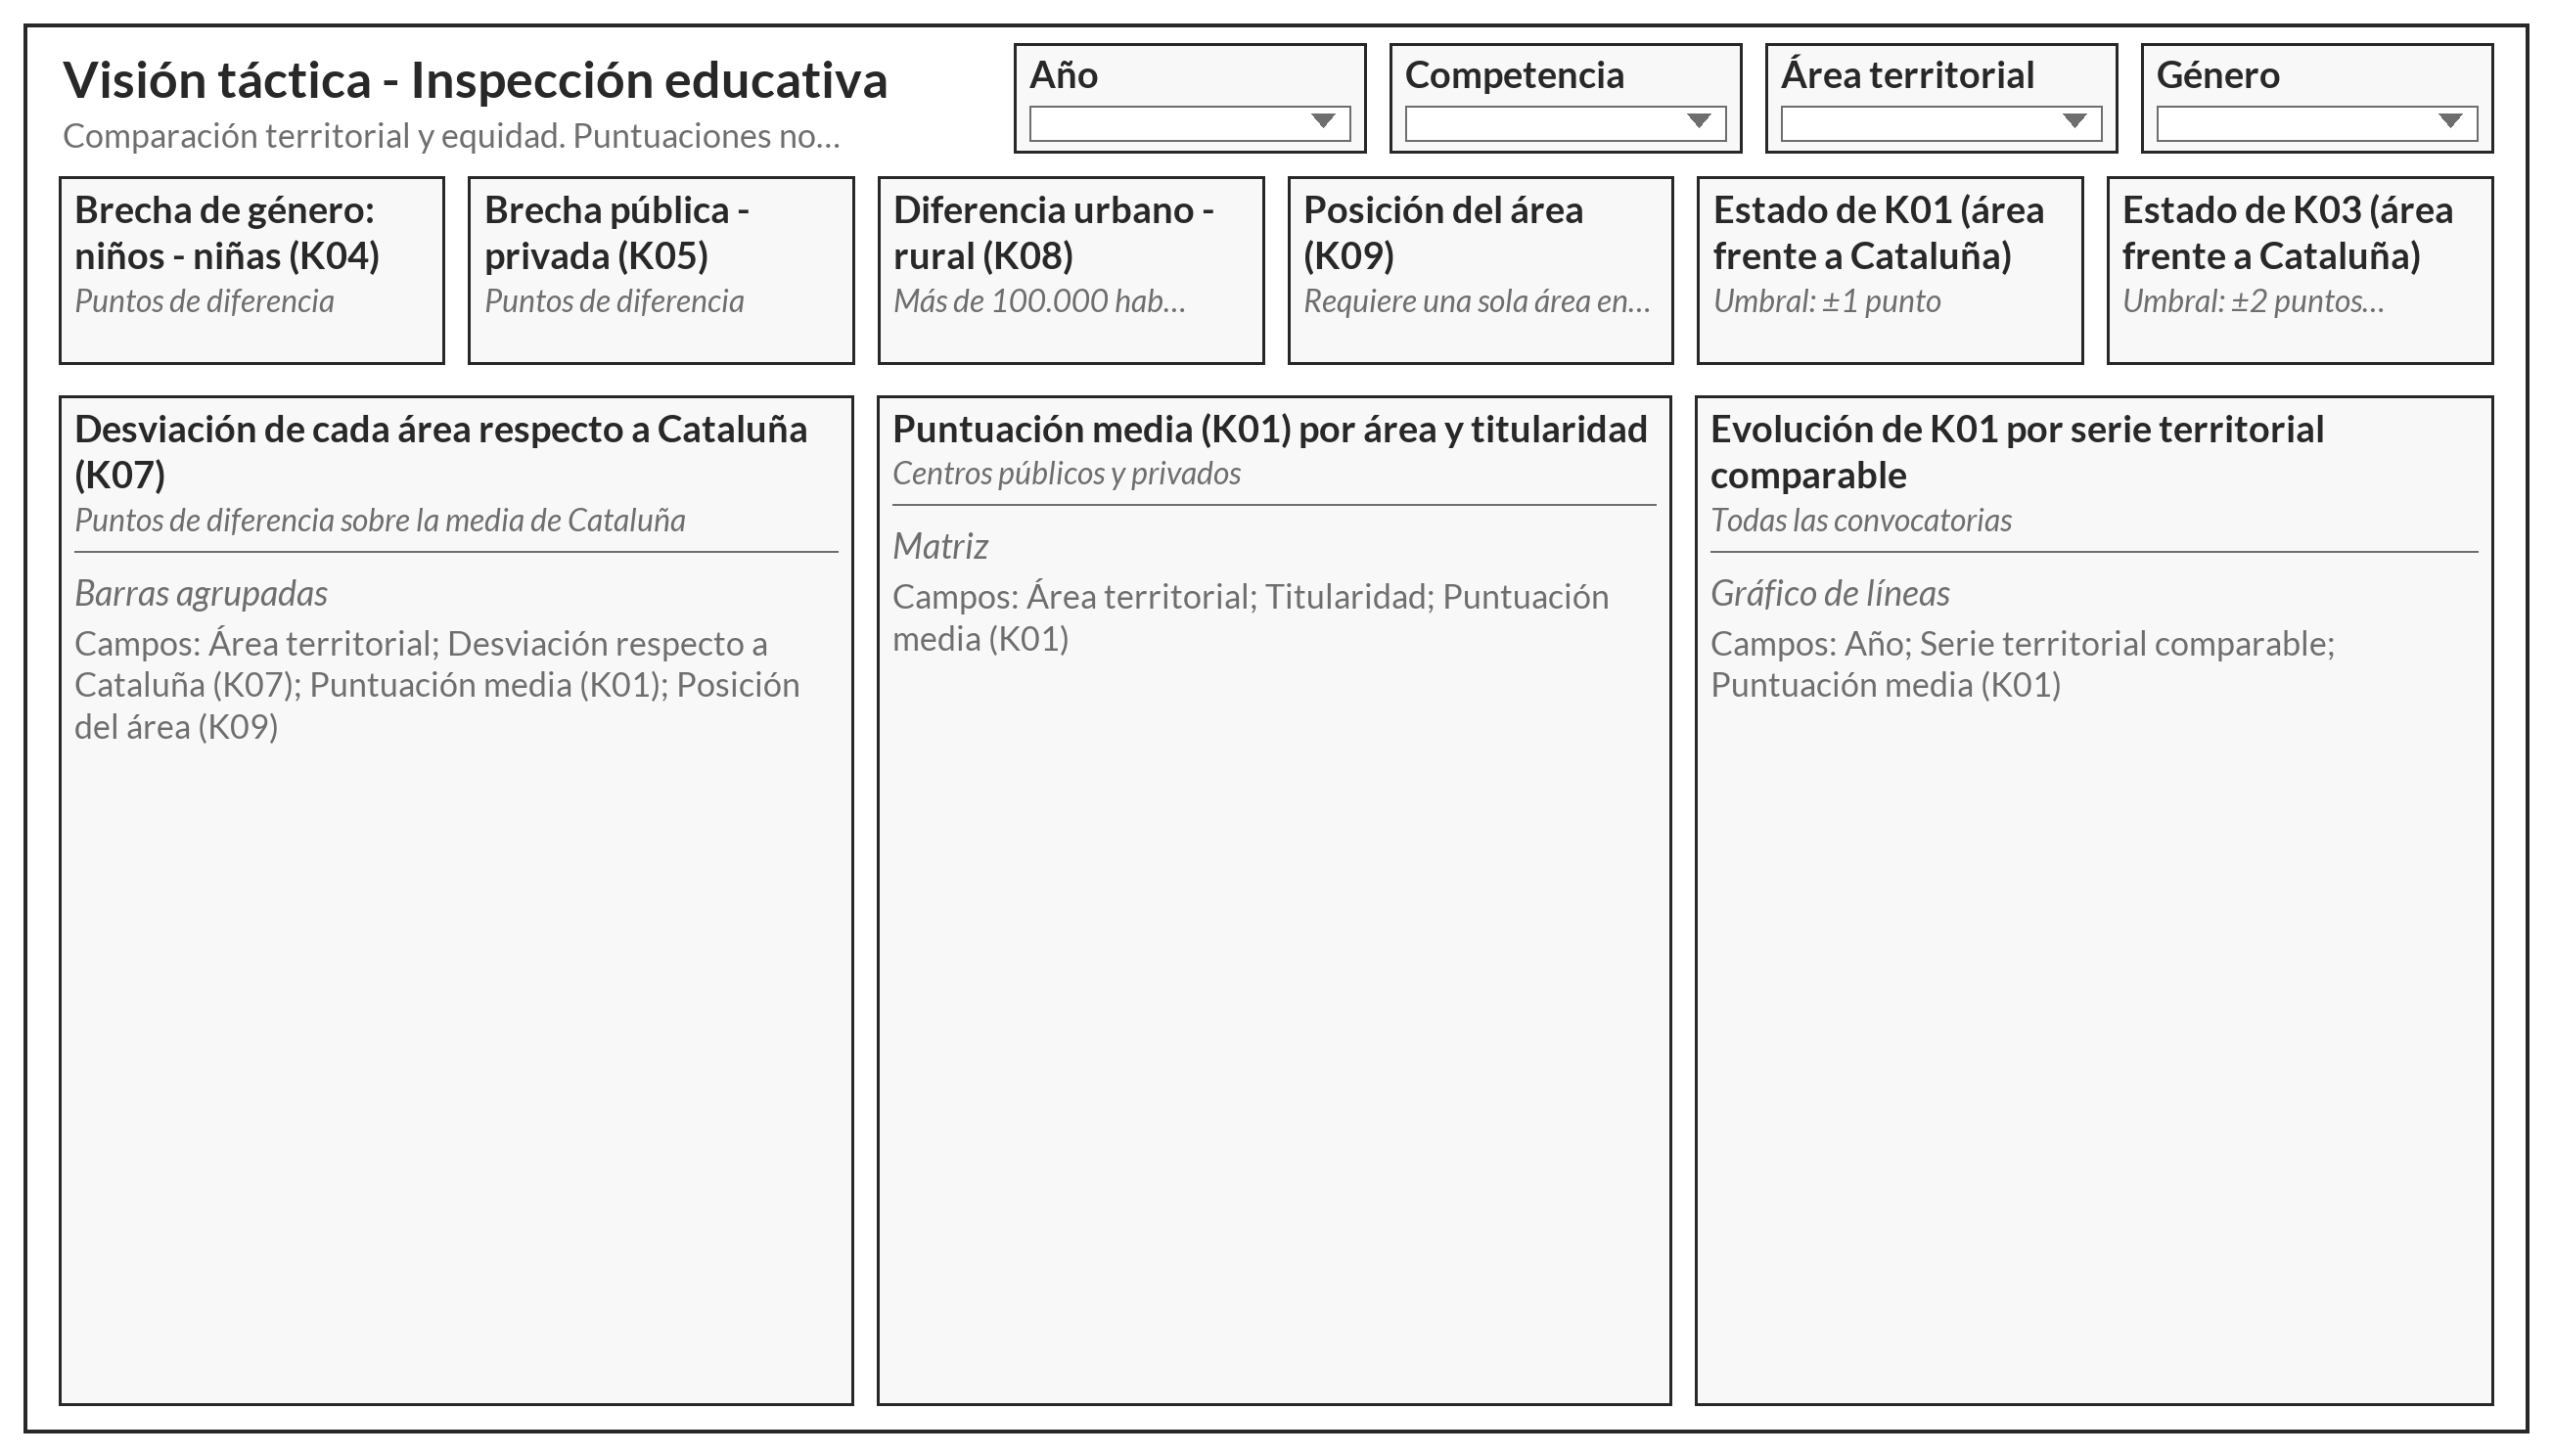
\includegraphics[width=\textwidth]{imagenes/diseno/panel_tactico.png}
\caption{Disposición final del panel táctico (inspección y coordinación territorial).}
\label{fig:panel_tactico}
\end{figure}

El panel táctico (Figura~\ref{fig:panel_tactico}) añade los segmentadores de área territorial y de género. Las tarjetas muestran las brechas (K04, K05 y K08), la posición del área (K09) y el estado de K01 y K03 del área frente a Cataluña. Las barras ordenan las áreas por su desviación respecto a Cataluña (K07), con la puntuación media y la posición en la descripción emergente. La matriz cruza el área con la titularidad, y el gráfico de evolución agrupa las áreas en series comparables.

\begin{figure}[H]
\centering
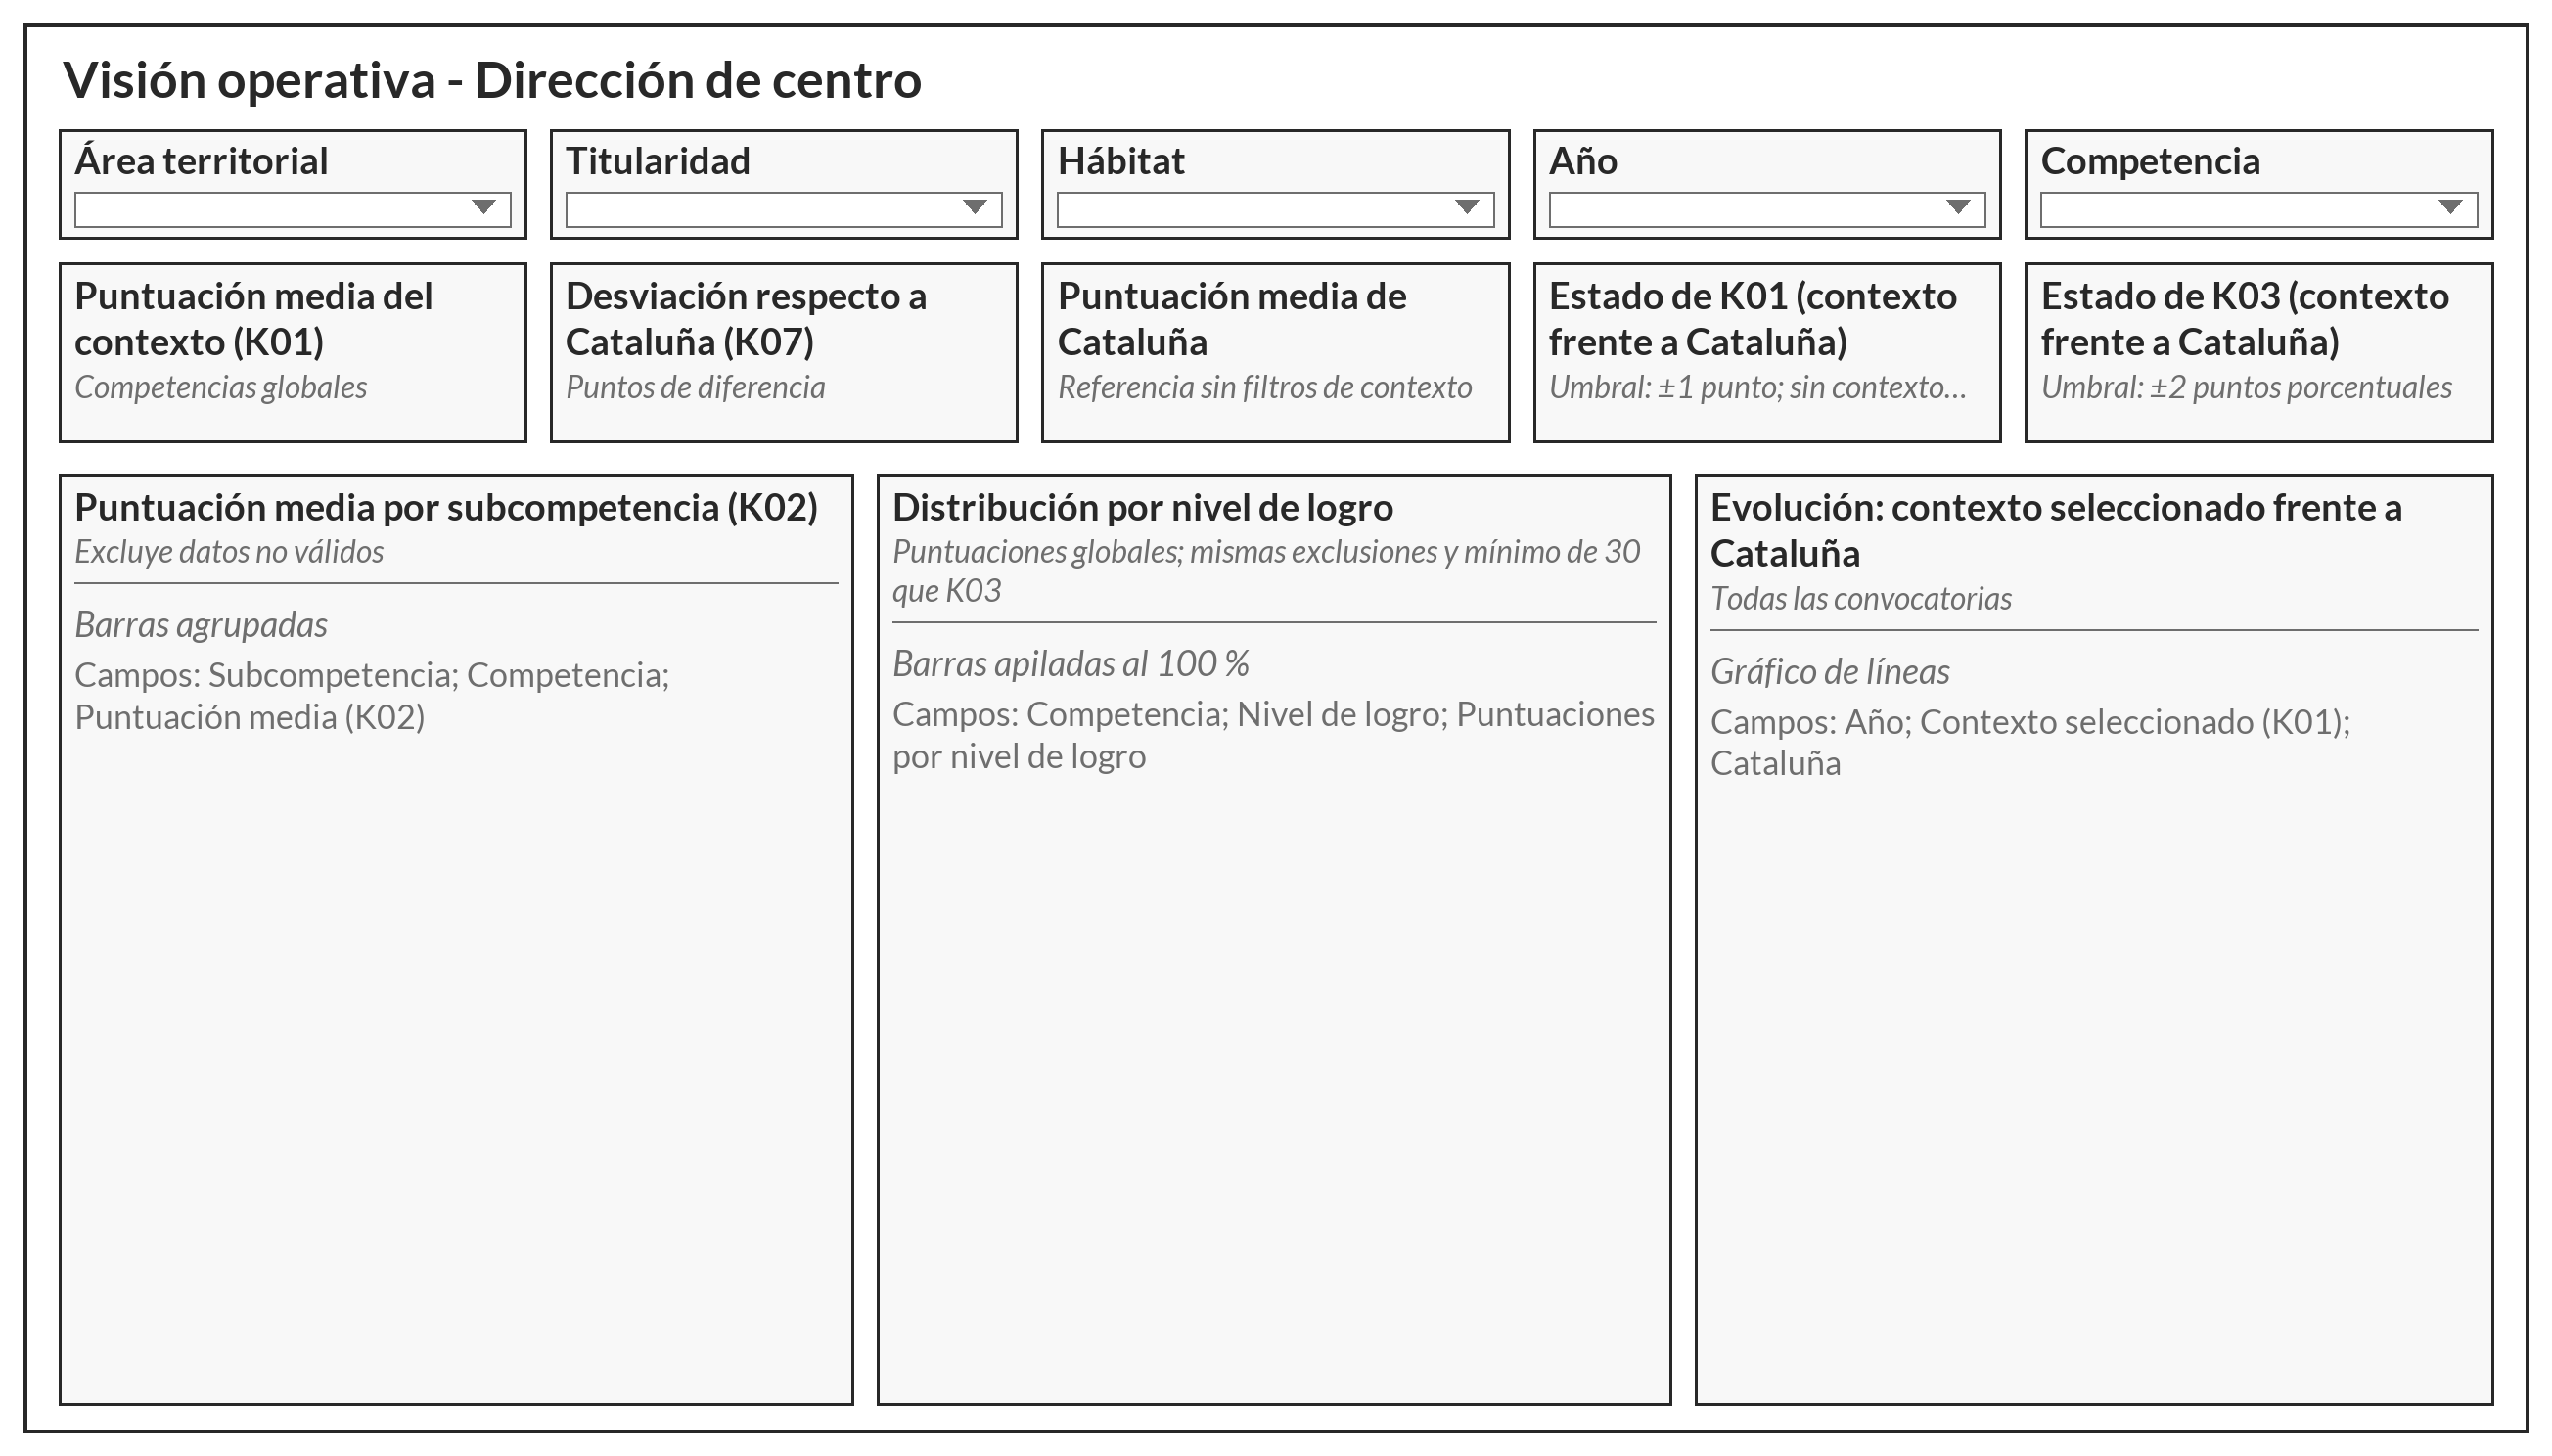
\includegraphics[width=\textwidth]{imagenes/diseno/panel_operativo.png}
\caption{Disposición final del panel operativo (dirección de centro).}
\label{fig:panel_operativo}
\end{figure}

El panel operativo (Figura~\ref{fig:panel_operativo}) tiene cinco segmentadores en una fila propia, porque el contexto del centro necesita tres (área, titularidad y hábitat) además del año y la competencia. Las tarjetas comparan K01 del contexto con la media de Cataluña, con la desviación (K07) y el estado de K01 y K03. Los gráficos muestran K02 por subcompetencia, la distribución por nivel de logro y la evolución del contexto frente a la de Cataluña.

El diseño final cambia el prototipo en los puntos siguientes. Todos se deben a lo que se aprendió al construir las medidas y al revisar el informe con los requisitos:
\begin{enumerate}
    \item En el panel estratégico solo se muestra el estado de la variación (K10). El prototipo lo ponía también en K01 y K03, pero sin un territorio con el que comparar el de K01 repetiría el de K10 y el de K03 valdría siempre neutro (Sección~\ref{sec:semaforos}). El estado de K01 y K03 está en los paneles táctico y operativo, donde se comparan con Cataluña.
    \item El panel táctico añade dos tarjetas con el estado de K01 y K03 del área y un segmentador de género, porque es el panel de la equidad. K04 ignora este filtro, ya que compara los dos géneros.
    \item La titularidad y el hábitat solo tienen segmentador en el panel operativo, y el género, en el táctico. RF06 los pedía en los tres paneles; en los demás se pueden aplicar desde el panel de filtros de Power BI, y con la sincronización se conservan al volver al panel que los tiene.
    \item La distribución por nivel de logro solo está en el panel operativo (RF12). El estratégico muestra K03 en una tarjeta y en la tabla por competencia; K03 es el tramo bajo de esa distribución.
    \item En los paneles táctico y operativo el aviso está en la cabecera y no al pie, para dejar más altura a los gráficos.
    \item Al seleccionar un área en el panel táctico, las barras de desviación siguen mostrando todas las áreas y no destacan la elegida. La posición y el estado del área aparecen en las tarjetas. Destacar la barra exigiría reglas de formato condicional que no se pueden comprobar fuera de Power BI Desktop.
    \item Sin ningún área ni contexto seleccionado, la desviación respecto a Cataluña vale 0, porque la selección es toda Cataluña, y el estado de K01 pasa a indicar la variación respecto a la convocatoria anterior.
\end{enumerate}

\section{Organización del repositorio}
\label{sec:organizacion_proyecto}
Todos los ficheros del proyecto están en un repositorio de Git alojado en GitHub. La Figura~\ref{fig:repositorio} muestra sus carpetas principales. La arquitectura general (Sección~\ref{sec:arquitectura}) describe las etapas del sistema; este apartado indica en qué ficheros está cada una.

\begin{figure}[!htbp]
\par\vspace{1ex}\noindent\begin{minipage}{\textwidth}\footnotesize\setstretch{1.0}
\begin{verbatim}
TFG_Project/
  Datos.zip                    fichero de origen comprimido
  Documentation/
    Docu_Final/Memoria/        memoria en LaTeX, figuras y compilar.sh (PDF y .docx)
    Docu_Final/Docu_Parcial/   informe de calidad, modelo y diccionario,
                               fichas de los KPIs, guía de uso
    Reuniones/, GEP/           notas de las reuniones y entregas de gestión
  PowerBI/                     proyecto de Power BI en formato .pbip (generado)
    CMI_Educacion_Primaria.SemanticModel/   modelo semántico en TMDL: tablas,
                                            consultas M, relaciones y medidas
    CMI_Educacion_Primaria.Report/          informe en PBIR: 3 páginas y 41 visuales
  trabajo_en_curso/
    generadores/               scripts que generan el modelo, las medidas,
                               el informe y las figuras de la memoria
    herramientas/              comprobación del modelo, las consultas y el informe
  validacion/                  validación independiente en Python: réplica de la
                               ETL, pruebas de integridad y KPIs de referencia
\end{verbatim}
\end{minipage}\par\vspace{1ex}
\caption{Carpetas principales del repositorio.}
\label{fig:repositorio}
\end{figure}

El proyecto de Power BI se guarda en formato \texttt{.pbip}, que separa el modelo semántico y el informe en ficheros de texto. El modelo se guarda en TMDL (\textit{Tabular Model Definition Language}), con un fichero por tabla. El informe se guarda en PBIR, con un fichero JSON por página y otro por elemento visual. Así cualquier cambio en una consulta, una medida o un visual aparece en el historial de Git como una diferencia de texto, y el repositorio no contiene ningún fichero \texttt{.pbix} (RNF10). Los datos no se versionan: \texttt{Datos.csv} ocupa 240 MB y se obtiene del fichero comprimido o del Portal de Datos Abiertos.

La carpeta \texttt{PowerBI/} no se edita a mano. Los scripts de \texttt{generadores/} escriben el modelo, las consultas, las medidas y el informe a partir de una sola fuente, de modo que un cambio se hace una vez y se regenera todo lo que depende de él. Los generadores conservan lo que Power BI Desktop añade al guardar el proyecto, como la configuración regional y la ruta local del fichero. Un cambio sigue siempre el mismo recorrido:
\begin{enumerate}
    \item Se modifica el generador o la consulta M correspondiente y se regenera el proyecto.
    \item Se ejecuta la validación independiente: la réplica de la ETL, las 31 pruebas de integridad y el cálculo de los KPIs de referencia, que se comparan con las medias oficiales.
    \item Se comprueban los ficheros generados con las bibliotecas y los esquemas oficiales de Microsoft: el modelo con TOM (\textit{Tabular Object Model}), las consultas con el analizador de Power Query y el informe con los esquemas JSON de PBIR.
    \item Se abre el proyecto en Power BI Desktop y se actualizan los datos.
\end{enumerate}

En la versión actual, el modelo pasa la validación de TOM sin errores, con 9 tablas, 20 medidas y 9 relaciones. Las 11 consultas M son correctas, los 49 ficheros del informe cumplen los esquemas y se superan las 31 pruebas de integridad. La comprobación de los paneles en Power BI Desktop se recogerá con el resto de la validación (Sección~\ref{sec:validacion}).

% ------------------------------------------
% CAPÍTULO 9: SOSTENIBILIDAD
% ------------------------------------------
\chapter{Sostenibilidad y compromiso social}
\begin{revisado}

\section{Autoevaluación}
Tras responder la encuesta de autoevaluación de la competencia de sostenibilidad, he valorado todas las cuestiones con la respuesta \textit{\guillemotleft{}Bastante\guillemotright{}}. El resultado indica un nivel intermedio-alto y homogéneo en las tres dimensiones: tengo una base sólida, pero aún no domino ninguna de ellas a nivel experto.

En la \textbf{dimensión económica}, el grado me ha dado herramientas para estimar costes, analizar la viabilidad y gestionar proyectos, y este TFG me ha obligado a construir un presupuesto por actividades con indicadores de control. Mi margen de mejora está en valorar los costes y beneficios a lo largo de toda la vida útil de un sistema, más allá de su desarrollo.

En la \textbf{dimensión social} conozco los principios de privacidad y protección de datos (RGPD) y soy consciente de que la tecnología puede reducir o ampliar desigualdades. Este proyecto me ha hecho reflexionar sobre cómo un indicador mal presentado puede estigmatizar a un territorio o a un tipo de centro. Me falta, sin embargo, experiencia en métodos para medir de forma objetiva el impacto social de una solución.

En la \textbf{dimensión ambiental} entiendo los conceptos de consumo energético, huella de carbono y ciclo de vida del hardware, pero hasta este proyecto no los había cuantificado en un desarrollo de software ni había considerado el coste ambiental de procesar datos en la nube.

Como \textbf{puntos fuertes} destaco que conozco las tres dimensiones por igual, que sé hacer un análisis económico y que tengo en cuenta la ética de los datos. Como \textbf{puntos débiles}, que ninguna respuesta alcance el nivel máximo refleja que mis conocimientos son más teóricos que aplicados: me cuesta traducirlos en indicadores medibles, especialmente en las dimensiones ambiental y social. En el TFG quiero aplicar estos conocimientos: tener en cuenta la sostenibilidad en las decisiones de diseño y documentar sus efectos.

\section{Matriz de sostenibilidad}
La Tabla~\ref{tab:matriz_sost} resume el análisis según la matriz de la FIB \cite{fib_sostenibilitat}, que cruza las tres dimensiones con el proyecto puesto en producción (PPP), la vida útil y los riesgos. Los apartados siguientes la desarrollan.

\begin{table}[H]
\centering
\small
\renewcommand{\arraystretch}{1.1}
\setlength{\tabcolsep}{3pt}
\begin{tabularx}{\textwidth}{@{} p{2.0cm} X X X @{}}
\toprule
\textbf{Dimensión} & \textbf{PPP} & \textbf{Vida útil} & \textbf{Riesgos} \\ \midrule
\textbf{Económica} & Presupuesto de 17.306,55 \texteuro{} (sin IVA) sin costes de licencia. & Ahorro de horas de análisis manual en el Departamento, la inspección y los centros. & Costes de licencias si se amplía a muchos usuarios con licencia Pro. \\ \addlinespace
\textbf{Ambiental} & 45,9 kWh y 11,5 kg de CO$_2$; se reutiliza hardware existente. & Datos procesados una sola vez y consumidos agregados, en lugar de que cada analista descargue y procese el fichero de 240 MB. & Crecimiento del volumen de datos y de los refrescos en la nube. \\ \addlinespace
\textbf{Social} & Formación de la estudiante en BI y en ética de datos. & Transparencia y detección de brechas de equidad. & Interpretación descontextualizada o estigmatización de territorios. \\ \bottomrule
\end{tabularx}
\caption{Matriz de sostenibilidad del proyecto.}
\label{tab:matriz_sost}
\end{table}

\section{Dimensión económica}
\textbf{PPP -- Reflexión sobre el coste estimado:} el coste del proyecto (17.306,55 \texteuro{} sin IVA) se concentra en un 83\% en personal, ya que el software es gratuito y el hardware ya existía. Es un coste razonable para un sistema BI de este alcance, y el detalle por tarea y las reservas de contingencia e imprevistos lo hacen realista.

\textbf{Vida útil -- Situación actual:} hoy el coste del análisis lo asume cada usuario: los equipos de inspección y de dirección dedican horas a descargar, filtrar y resumir los datos en hojas de cálculo, sin poder reutilizar el trabajo de otros.

\textbf{Mejora económica:} el CMI centraliza ese trabajo. Como hipótesis prudente, si solo un 10\% de los más de 2.000 centros con primaria de Cataluña lo usaran y ahorraran 2 horas al año (a 30 \texteuro{}/h), el ahorro sería de unos 12.000 \texteuro{} anuales, a los que se suma el ahorro de la inspección. Como los datos son públicos y anónimos, el panel puede publicarse en la web con una única licencia Pro \cite{ms_powerbi_pricing}, de modo que el coste de explotación es muy bajo (una licencia y unas 20 horas anuales para cargar cada nueva convocatoria). Con estos supuestos, la inversión se recuperaría en un plazo de uno a dos años.

\section{Dimensión ambiental}
\textbf{PPP -- Impacto estimado:} el consumo eléctrico del desarrollo será de $540\ \text{h} \times 0{,}085\ \text{kWh/h} = 45{,}9$ kWh. Con un factor de emisión conservador de 0,25 kg de CO$_2$/kWh, superior al del mix de generación publicado por REE en los últimos años \cite{ree_emisiones}, la huella será de unos $11{,}5$ kg de CO$_2$.

\textbf{Minimización del impacto:} se reutiliza un portátil existente, sin comprar hardware nuevo; se reutilizan datos abiertos ya recogidos, sin nuevas campañas de recogida; el trabajo es en remoto, sin desplazamientos; y el modelo se optimiza eliminando columnas innecesarias para reducir la memoria y la CPU necesarias en cada consulta.

\textbf{Vida útil -- Situación actual y mejora:} actualmente cada analista descarga el fichero completo (240 MB) y lo procesa en su equipo, repitiendo el mismo cálculo muchas veces. Con el CMI los datos se transforman una sola vez y los usuarios consumen agregados comprimidos, lo que reduce el tráfico de datos y el procesamiento redundante. Además, los paneles interactivos sustituyen la impresión de informes.

\section{Dimensión social}
\textbf{PPP -- Aportación personal:} el proyecto me permitirá consolidar competencias de ingeniería de datos, modelado dimensional y diseño de cuadros de mando, muy demandadas en el mercado laboral, y aprender a usar los datos públicos de forma ética.

\textbf{Vida útil -- Situación actual y mejora:} hoy la información sobre los resultados educativos llega en formatos poco accesibles para perfiles no técnicos. El CMI facilita el acceso a esa información y permite identificar brechas de género, de titularidad y territoriales, para orientar los recursos de refuerzo de manera más justa. Para evitar la estigmatización, los paneles mostrarán siempre los datos en su contexto (hábitat, naturaleza) y no permitirán identificar a centros ni a alumnos (RGPD).

\textbf{Necesidad real:} sí existe. La administración educativa promueve la toma de decisiones basada en datos \cite{mandinach2012data}, publica los microdatos como datos abiertos y, sin embargo, no dispone de una herramienta interactiva orientada a objetivos para explotarlos.

\end{revisado}

% ------------------------------------------
% BIBLIOGRAFÍA (ESTILO IEEE)
% ------------------------------------------
\bibliographystyle{IEEEtran}
\bibliography{bibliografia}

\end{document}
